% Options for packages loaded elsewhere
\PassOptionsToPackage{unicode}{hyperref}
\PassOptionsToPackage{hyphens}{url}
\PassOptionsToPackage{dvipsnames,svgnames,x11names}{xcolor}
%
\documentclass[
  a4paper,
]{scrreport}

\usepackage{amsmath,amssymb}
\usepackage{lmodern}
\usepackage{iftex}
\ifPDFTeX
  \usepackage[T1]{fontenc}
  \usepackage[utf8]{inputenc}
  \usepackage{textcomp} % provide euro and other symbols
\else % if luatex or xetex
  \usepackage{unicode-math}
  \defaultfontfeatures{Scale=MatchLowercase}
  \defaultfontfeatures[\rmfamily]{Ligatures=TeX,Scale=1}
\fi
% Use upquote if available, for straight quotes in verbatim environments
\IfFileExists{upquote.sty}{\usepackage{upquote}}{}
\IfFileExists{microtype.sty}{% use microtype if available
  \usepackage[]{microtype}
  \UseMicrotypeSet[protrusion]{basicmath} % disable protrusion for tt fonts
}{}
\makeatletter
\@ifundefined{KOMAClassName}{% if non-KOMA class
  \IfFileExists{parskip.sty}{%
    \usepackage{parskip}
  }{% else
    \setlength{\parindent}{0pt}
    \setlength{\parskip}{6pt plus 2pt minus 1pt}}
}{% if KOMA class
  \KOMAoptions{parskip=half}}
\makeatother
\usepackage{xcolor}
\setlength{\emergencystretch}{3em} % prevent overfull lines
\setcounter{secnumdepth}{5}
% Make \paragraph and \subparagraph free-standing
\ifx\paragraph\undefined\else
  \let\oldparagraph\paragraph
  \renewcommand{\paragraph}[1]{\oldparagraph{#1}\mbox{}}
\fi
\ifx\subparagraph\undefined\else
  \let\oldsubparagraph\subparagraph
  \renewcommand{\subparagraph}[1]{\oldsubparagraph{#1}\mbox{}}
\fi


\providecommand{\tightlist}{%
  \setlength{\itemsep}{0pt}\setlength{\parskip}{0pt}}\usepackage{longtable,booktabs,array}
\usepackage{calc} % for calculating minipage widths
% Correct order of tables after \paragraph or \subparagraph
\usepackage{etoolbox}
\makeatletter
\patchcmd\longtable{\par}{\if@noskipsec\mbox{}\fi\par}{}{}
\makeatother
% Allow footnotes in longtable head/foot
\IfFileExists{footnotehyper.sty}{\usepackage{footnotehyper}}{\usepackage{footnote}}
\makesavenoteenv{longtable}
\usepackage{graphicx}
\makeatletter
\def\maxwidth{\ifdim\Gin@nat@width>\linewidth\linewidth\else\Gin@nat@width\fi}
\def\maxheight{\ifdim\Gin@nat@height>\textheight\textheight\else\Gin@nat@height\fi}
\makeatother
% Scale images if necessary, so that they will not overflow the page
% margins by default, and it is still possible to overwrite the defaults
% using explicit options in \includegraphics[width, height, ...]{}
\setkeys{Gin}{width=\maxwidth,height=\maxheight,keepaspectratio}
% Set default figure placement to htbp
\makeatletter
\def\fps@figure{htbp}
\makeatother

\usepackage{venndiagram}
\newcommand{\NN}{\mathbb{N}}
\newcommand{\ZZ}{\mathbb{Z}}
\newcommand{\QQ}{\mathbb{Q}}
\newcommand{\RR}{\mathbb{R}}
\newcommand{\CC}{\mathbb{C}}
\DeclareMathOperator{\operatorname{Int}}{Int}
\DeclareMathOperator{\operatorname{Ext}}{Ext}
\DeclareMathOperator{\operatorname{Fr}}{Fr}
\DeclareMathOperator{\Adh}{Adh}
\DeclareMathOperator{\Ac}{Ac}
\DeclareMathOperator{\sen}{sen}
\makeatletter
\@ifpackageloaded{tcolorbox}{}{\usepackage[many]{tcolorbox}}
\@ifpackageloaded{fontawesome5}{}{\usepackage{fontawesome5}}
\definecolor{quarto-callout-color}{HTML}{909090}
\definecolor{quarto-callout-note-color}{HTML}{0758E5}
\definecolor{quarto-callout-important-color}{HTML}{CC1914}
\definecolor{quarto-callout-warning-color}{HTML}{EB9113}
\definecolor{quarto-callout-tip-color}{HTML}{00A047}
\definecolor{quarto-callout-caution-color}{HTML}{FC5300}
\definecolor{quarto-callout-color-frame}{HTML}{acacac}
\definecolor{quarto-callout-note-color-frame}{HTML}{4582ec}
\definecolor{quarto-callout-important-color-frame}{HTML}{d9534f}
\definecolor{quarto-callout-warning-color-frame}{HTML}{f0ad4e}
\definecolor{quarto-callout-tip-color-frame}{HTML}{02b875}
\definecolor{quarto-callout-caution-color-frame}{HTML}{fd7e14}
\makeatother
\makeatletter
\@ifpackageloaded{tikz}{}{\usepackage{tikz}}
\makeatother
\makeatletter
\@ifpackageloaded{bookmark}{}{\usepackage{bookmark}}
\makeatother
\makeatletter
\@ifpackageloaded{caption}{}{\usepackage{caption}}
\AtBeginDocument{%
\ifdefined\contentsname
  \renewcommand*\contentsname{Tabla de contenidos}
\else
  \newcommand\contentsname{Tabla de contenidos}
\fi
\ifdefined\listfigurename
  \renewcommand*\listfigurename{Listado de Figuras}
\else
  \newcommand\listfigurename{Listado de Figuras}
\fi
\ifdefined\listtablename
  \renewcommand*\listtablename{Listado de Tablas}
\else
  \newcommand\listtablename{Listado de Tablas}
\fi
\ifdefined\figurename
  \renewcommand*\figurename{Figura}
\else
  \newcommand\figurename{Figura}
\fi
\ifdefined\tablename
  \renewcommand*\tablename{Tabla}
\else
  \newcommand\tablename{Tabla}
\fi
}
\@ifpackageloaded{float}{}{\usepackage{float}}
\floatstyle{ruled}
\@ifundefined{c@chapter}{\newfloat{codelisting}{h}{lop}}{\newfloat{codelisting}{h}{lop}[chapter]}
\floatname{codelisting}{Listado}
\newcommand*\listoflistings{\listof{codelisting}{Listado de Listados}}
\usepackage{amsthm}
\theoremstyle{definition}
\newtheorem{exercise}{Ejercicio}[chapter]
\theoremstyle{remark}
\renewcommand*{\proofname}{Prueba}
\newtheorem*{remark}{Observación}
\newtheorem*{solution}{Solución}
\makeatother
\makeatletter
\@ifpackageloaded{caption}{}{\usepackage{caption}}
\@ifpackageloaded{subcaption}{}{\usepackage{subcaption}}
\makeatother
\makeatletter
\@ifpackageloaded{tcolorbox}{}{\usepackage[many]{tcolorbox}}
\makeatother
\makeatletter
\@ifundefined{shadecolor}{\definecolor{shadecolor}{rgb}{.97, .97, .97}}
\makeatother
\makeatletter
\makeatother
\ifLuaTeX
\usepackage[bidi=basic]{babel}
\else
\usepackage[bidi=default]{babel}
\fi
\babelprovide[main,import]{spanish}
% get rid of language-specific shorthands (see #6817):
\let\LanguageShortHands\languageshorthands
\def\languageshorthands#1{}
\ifLuaTeX
  \usepackage{selnolig}  % disable illegal ligatures
\fi
\IfFileExists{bookmark.sty}{\usepackage{bookmark}}{\usepackage{hyperref}}
\IfFileExists{xurl.sty}{\usepackage{xurl}}{} % add URL line breaks if available
\urlstyle{same} % disable monospaced font for URLs
\hypersetup{
  pdftitle={Problemas de Análisis Matemático},
  pdfauthor={Alfredo Sánchez Alberca},
  pdflang={es},
  colorlinks=true,
  linkcolor={blue},
  filecolor={Maroon},
  citecolor={Blue},
  urlcolor={Blue},
  pdfcreator={LaTeX via pandoc}}

\title{Problemas de Análisis Matemático}
\author{Alfredo Sánchez Alberca}
\date{6/1/22}

\begin{document}
\begin{titlepage}

%\AddToShipoutPicture*{\put(0,0){\includegraphics[scale=0.8]{img/background2}}} % Imagen de fondo, requiere el paquete eso-pic.
\begin{center}
\vspace*{5cm}

\Huge
{\textbf{\textsf{Problemas de Análisis Matemático}}}

\vspace{0.5cm}
\LARGE
{\textbf{\textsf{}}}

\vspace{1.5cm}


\includegraphics[width=0.4\textwidth]{img/logos/sticker.png}
\end{center}

\vfill

\begin{flushleft}
\begin{tabular}{ll}

\includegraphics[width=0.1\textwidth]{img/logos/aprendeconalf.png} & \parbox[b]{5cm}{\Large\textsf{Alfredo
Sánchez
Alberca}\\ \textsf{asalber@ceu.es} \\ \textsf{https://aprendeconalf.es}}
\end{tabular}
\end{flushleft}
\end{titlepage}\ifdefined\Shaded\renewenvironment{Shaded}{\begin{tcolorbox}[boxrule=0pt, borderline west={3pt}{0pt}{shadecolor}, sharp corners, interior hidden, frame hidden, breakable, enhanced]}{\end{tcolorbox}}\fi

\renewcommand*\contentsname{Tabla de contenidos}
{
\hypersetup{linkcolor=}
\setcounter{tocdepth}{2}
\tableofcontents
}
\bookmarksetup{startatroot}

\hypertarget{prefacio}{%
\chapter*{Prefacio}\label{prefacio}}
\addcontentsline{toc}{chapter}{Prefacio}

\markboth{Prefacio}{Prefacio}

Colección de problemas de Análisis Matemático aplicado.

\bookmarksetup{startatroot}

\hypertarget{teoruxeda-de-conjuntos}{%
\chapter{Teoría de conjuntos}\label{teoruxeda-de-conjuntos}}

\leavevmode\vadjust pre{\hypertarget{exr-operaciones-conjuntos}{}}%
\begin{exercise}[]\label{exr-operaciones-conjuntos}

Dado el conjunto universo de los números de un dado
\(\Omega=\{1, 2, 3, 4, 5, 6\}\) y los subconjuntos correspondientes a
sacar par en el lanzamiento de un dado \(A=\{2, 4, 6\}\) y sacar menos
de 5 en el lanzamiento de un dado \(B=\{1, 2, 3, 4\}\), calcular e
interpretar los siguientes conjuntos:

\begin{enumerate}
\def\labelenumi{\alph{enumi}.}
\tightlist
\item
  \(A\cup B\)
\item
  \(A\cap B\)
\item
  \(\overline A\) y \(\overline B\)
\item
  \(A-B\) y \(B-A\)
\item
  \(A\triangle B\)
\item
  \(\overline{(A\cup B)}\)
\item
  \(\overline{(A\cap B)}\)
\item
  \(A\cup \overline B\)
\item
  \(\overline{\overline A \cap B}\)
\end{enumerate}

¿Qué conjuntos de números en el lanzamiento de un dado serían disjuntos
con \(A\)? ¿Y con \(A\cup B\)?

\end{exercise}

\begin{tcolorbox}[enhanced jigsaw, leftrule=.75mm, rightrule=.15mm, colbacktitle=quarto-callout-tip-color!10!white, opacitybacktitle=0.6, bottomtitle=1mm, coltitle=black, colback=white, titlerule=0mm, left=2mm, arc=.35mm, breakable, colframe=quarto-callout-tip-color-frame, toprule=.15mm, toptitle=1mm, opacityback=0, title=\textcolor{quarto-callout-tip-color}{\faLightbulb}\hspace{0.5em}{Solución}, bottomrule=.15mm]

\begin{enumerate}
\def\labelenumi{\alph{enumi}.}
\tightlist
\item
  \(A\cup B = \{1, 2, 3, 4, 6\}\)
\item
  \(A\cap B = \{2, 4\}\)
\item
  \(\overline A = \{1, 3, 5\}\) y \(\overline B = \{5, 6\}\)
\item
  \(A-B = \{6\}\) y \(B-A = \{1,3\}\)
\item
  \(A\triangle B = \{1, 3, 6\}\)
\item
  \(\overline{(A\cup B)} = \{5\}\)
\item
  \(\overline{(A\cap B)} = \{1,3, 5, 6\}\)
\item
  \(A\cup \overline B = \{2, 4, 5, 6\}\)
\item
  \(\overline{\overline A \cap B} = \{2, 4, 5, 6\}\)
\end{enumerate}

Serían disjuntos con \(A\) todos los conjuntos que solo tuviesen alguno
de los números \(1\), \(3\) o \(5\), por ejemplo el conjunto
\(\{1, 5\}\). El único conjunto disjunto con \(A\cup B\), además del
vacío es \(\{5\}\).

\end{tcolorbox}

\leavevmode\vadjust pre{\hypertarget{exr-expresion-conjuntos}{}}%
\begin{exercise}[]\label{exr-expresion-conjuntos}

Expresar con operaciones entre los conjuntos \(A\), \(B\) y \(C\), los
conjuntos que se corresponden con las regiones sombreadas en los
siguientes diagramas.

\end{exercise}

\begin{figure}

\begin{minipage}[t]{0.33\linewidth}

{\centering 

\raisebox{-\height}{

\begin{venndiagram3sets}[showframe=false,shade=blue!20]
\fillOnlyB
\fillCCapB
\end{venndiagram3sets}


}

\caption{a.}

}

\end{minipage}%
%
\begin{minipage}[t]{0.33\linewidth}

{\centering 

\raisebox{-\height}{

\usepackage{venndiagram}

\begin{venndiagram3sets}[showframe=false,shade=blue!20]
\fillOnlyA
\fillOnlyC
\fillACapB
\end{venndiagram3sets}


}

\caption{b.}

}

\end{minipage}%
%
\begin{minipage}[t]{0.33\linewidth}

{\centering 

\raisebox{-\height}{

\begin{venndiagram3sets}[showframe=false,shade=blue!20]
\fillOnlyA
\fillOnlyB
\fillOnlyC
\end{venndiagram3sets}


}

\caption{b.}

}

\end{minipage}%

\end{figure}

\begin{tcolorbox}[enhanced jigsaw, leftrule=.75mm, rightrule=.15mm, colbacktitle=quarto-callout-tip-color!10!white, opacitybacktitle=0.6, bottomtitle=1mm, coltitle=black, colback=white, titlerule=0mm, left=2mm, arc=.35mm, breakable, colframe=quarto-callout-tip-color-frame, toprule=.15mm, toptitle=1mm, opacityback=0, title=\textcolor{quarto-callout-tip-color}{\faLightbulb}\hspace{0.5em}{Solución}, bottomrule=.15mm]

\begin{enumerate}
\def\labelenumi{\alph{enumi}.}
\tightlist
\item
  \((B-A)\cup (A\cap B\cap C)\)
\item
  \((A\cup B)\cap \overline{(A\cap C)}\cap \overline{(B\cap C)}\cup (A\cap B\cap C)\)
\item
  \((A\cup B\cup C) - ((A\cap B)\cup (A\cap C)\cup (B\cap C))\)
\end{enumerate}

\end{tcolorbox}

\leavevmode\vadjust pre{\hypertarget{exr-leyes-morgan}{}}%
\begin{exercise}[]\label{exr-leyes-morgan}

Demostrar gráficamente las leyes de Morgan
\(\overline{A\cup B}=\overline A \cap \overline B\) y
\(\overline{A\cap B}=\overline A \cup \overline B\).

\end{exercise}

\leavevmode\vadjust pre{\hypertarget{exr-conjunto-potencia}{}}%
\begin{exercise}[]\label{exr-conjunto-potencia}

Construir por extensión el conjunto potencia del conjunto de los grupos
sanguíneos \(S=\{0, A, B, AB\}\). ¿Cuál es su cardinal?

\end{exercise}

\begin{tcolorbox}[enhanced jigsaw, leftrule=.75mm, rightrule=.15mm, colbacktitle=quarto-callout-tip-color!10!white, opacitybacktitle=0.6, bottomtitle=1mm, coltitle=black, colback=white, titlerule=0mm, left=2mm, arc=.35mm, breakable, colframe=quarto-callout-tip-color-frame, toprule=.15mm, toptitle=1mm, opacityback=0, title=\textcolor{quarto-callout-tip-color}{\faLightbulb}\hspace{0.5em}{Solución}, bottomrule=.15mm]

\begin{align*}
\mathcal{P}(S)&=\{\emptyset, \{A\}, \{B\}, \{AB\}, \\
& \{\emptyset,A\},\{\emptyset,B\}, \{\emptyset,AB\}, \{A,B\}, \{A,AB\}, \{B,AB\}, \{\emptyset,A,B\},\\ 
& \{\emptyset,A,AB\}, \{\emptyset,B,AB\}, \{A,B,AB\}, \\ 
& \{\emptyset,A,B,AB\} \}
\end{align*}

\end{tcolorbox}

\leavevmode\vadjust pre{\hypertarget{exr-producto-cartesiano-grupos-sanguineos}{}}%
\begin{exercise}[]\label{exr-producto-cartesiano-grupos-sanguineos}

Construir el producto cartesiano del conjunto d los grupos sanguíneos
\(S=\{0, A, B, AB\}\) y el conjunto de los factores Rh
\(R=\{\mbox{Rh}+, \mbox{Rh}-\}\).

\end{exercise}

\begin{tcolorbox}[enhanced jigsaw, leftrule=.75mm, rightrule=.15mm, colbacktitle=quarto-callout-tip-color!10!white, opacitybacktitle=0.6, bottomtitle=1mm, coltitle=black, colback=white, titlerule=0mm, left=2mm, arc=.35mm, breakable, colframe=quarto-callout-tip-color-frame, toprule=.15mm, toptitle=1mm, opacityback=0, title=\textcolor{quarto-callout-tip-color}{\faLightbulb}\hspace{0.5em}{Solución}, bottomrule=.15mm]

\begin{align*}
S \times R &=\{(0,\mbox{Rh}+), (0,\mbox{Rh}-), (A,\mbox{Rh}+)), (A,\mbox{Rh}-),\\
& (B,\mbox{Rh}+), (B,\mbox{Rh}-), (AB,\mbox{Rh}+), (AB,\mbox{Rh}-) \}
\end{align*}

\end{tcolorbox}

\leavevmode\vadjust pre{\hypertarget{exr-relacion-equivalencia-1}{}}%
\begin{exercise}[]\label{exr-relacion-equivalencia-1}

Demostrar que la relación
\(R=\{(x,y)\in \mathbb{Z}^2: x-y \mbox{ es par}\}\) es una relación de
equivalencia.

\end{exercise}

\begin{tcolorbox}[enhanced jigsaw, leftrule=.75mm, rightrule=.15mm, colbacktitle=quarto-callout-tip-color!10!white, opacitybacktitle=0.6, bottomtitle=1mm, coltitle=black, colback=white, titlerule=0mm, left=2mm, arc=.35mm, breakable, colframe=quarto-callout-tip-color-frame, toprule=.15mm, toptitle=1mm, opacityback=0, title=\textcolor{quarto-callout-tip-color}{\faLightbulb}\hspace{0.5em}{Solución}, bottomrule=.15mm]

\emph{Propiedad reflexiva}: \(\forall a\in\mathbb{Z}\) \(a-a=0\) es par,
de manera que \(aRa\).\\
\emph{Propiedad simétrica}: \(\forall a,b\in\mathbb{Z}\) si \(aRb\)
entonces \(a-b\) es par, es decir, existe \(k\in \mathbb{Z}\) tal que
\(a-b=2k\). Por tanto, \(b-a=2(-k)\) también es par y \(bRa\).
\emph{Propiedad transitiva}: \(\forall a,b,c\in\mathbb{Z}\), si \(aRb\)
y \(bRc\) entonces \(a-b\) y \(b-c\) son pares, de manera que su suma
\(a-b+b-c = a-c\) también es par, y \(aRc\).

\end{tcolorbox}

\leavevmode\vadjust pre{\hypertarget{exr-relaciones-equivalencia}{}}%
\begin{exercise}[]\label{exr-relaciones-equivalencia}

¿Cuáles de las siguientes relaciones son relaciones de equivalencia?
¿Cuáles don de orden?

\begin{enumerate}
\def\labelenumi{\alph{enumi}.}
\tightlist
\item
  \(R_1=\{(x,y)\in \mathbb{R}^2: x = y\}\)
\item
  \(R_2=\{(x,y)\in \mathbb{R}^2: x\leq y\}\)
\item
  \(R_3=\{(x,y)\in \mathbb{R}^2: x^2 + y^2 = 1\}\)
\item
  \(R_4=\{(x,y)\in \mathbb{R}^2: x^2 + y^2 \leq 1\}\)
\end{enumerate}

\end{exercise}

\begin{tcolorbox}[enhanced jigsaw, leftrule=.75mm, rightrule=.15mm, colbacktitle=quarto-callout-tip-color!10!white, opacitybacktitle=0.6, bottomtitle=1mm, coltitle=black, colback=white, titlerule=0mm, left=2mm, arc=.35mm, breakable, colframe=quarto-callout-tip-color-frame, toprule=.15mm, toptitle=1mm, opacityback=0, title=\textcolor{quarto-callout-tip-color}{\faLightbulb}\hspace{0.5em}{Solución}, bottomrule=.15mm]

\begin{enumerate}
\def\labelenumi{\alph{enumi}.}
\tightlist
\item
  \(R_1\) es relación de equivalencia.
\item
  \(R_2\) es relación de orden.
\item
  \(R_3\) no es relación de equivalencia ni de orden porque no cumple
  las propiedades reflexiva y transitiva.
\item
  \(R_4\) es no es relación de equivalencia ni de orden porque tampoco
  cumple las propiedades reflexiva y transitiva.
\end{enumerate}

\end{tcolorbox}

\leavevmode\vadjust pre{\hypertarget{exr-supremo-infimo-maximo-minimo}{}}%
\begin{exercise}[]\label{exr-supremo-infimo-maximo-minimo}

\(\star\) Para cada uno de los conjuntos siguientes, calcular si existe
el supremo, el ínfimo, el máximo y el mínimo.

\begin{enumerate}
\def\labelenumi{\alph{enumi}.}
\tightlist
\item
  \(A=\{1, 2, 3, 4, 5\}\)
\item
  \(B=\{x\in\mathbb{N} : x \mbox{ es par}\}\)
\item
  \(C=\{x\in\mathbb{Q} : 0< x \leq 1\}\)
\end{enumerate}

\end{exercise}

\begin{tcolorbox}[enhanced jigsaw, leftrule=.75mm, rightrule=.15mm, colbacktitle=quarto-callout-tip-color!10!white, opacitybacktitle=0.6, bottomtitle=1mm, coltitle=black, colback=white, titlerule=0mm, left=2mm, arc=.35mm, breakable, colframe=quarto-callout-tip-color-frame, toprule=.15mm, toptitle=1mm, opacityback=0, title=\textcolor{quarto-callout-tip-color}{\faLightbulb}\hspace{0.5em}{Solución}, bottomrule=.15mm]

\begin{enumerate}
\def\labelenumi{\alph{enumi}.}
\tightlist
\item
  \(\sup(A)=5\), \(\inf(A) = 1\), \(\max(A)=5\), \(\min(A)=1\).
\item
  \(\inf(B) = 2\) y \(\min(B)=2\). No existe el supremo ni el máximo
  porque \(B\) no está acotado superiormente.
\item
  \(\sup(C)=1\), \(\inf(C) = 0\) y \(\max(C)=1\). No existe el mínimo.
\end{enumerate}

\end{tcolorbox}

\leavevmode\vadjust pre{\hypertarget{exr-ejemplos-funciones}{}}%
\begin{exercise}[]\label{exr-ejemplos-funciones}

\(\star\) Dar ejemplos de funciones
\(f:\mathbb{Z}\rightarrow \mathbb{Z}\) que cumplan lo siguiente:

\begin{enumerate}
\def\labelenumi{\alph{enumi}.}
\tightlist
\item
  \(f\) es inyectiva pero no sobreyectiva.
\item
  \(f\) es sobreyectiva pero no inyectiva.
\item
  \(f\) no es inyectiva ni sobreyectiva.
\item
  \(f\) es biyectiva y distinta de la función identidad.
\end{enumerate}

\end{exercise}

\begin{tcolorbox}[enhanced jigsaw, leftrule=.75mm, rightrule=.15mm, colbacktitle=quarto-callout-tip-color!10!white, opacitybacktitle=0.6, bottomtitle=1mm, coltitle=black, colback=white, titlerule=0mm, left=2mm, arc=.35mm, breakable, colframe=quarto-callout-tip-color-frame, toprule=.15mm, toptitle=1mm, opacityback=0, title=\textcolor{quarto-callout-tip-color}{\faLightbulb}\hspace{0.5em}{Solución}, bottomrule=.15mm]

\begin{enumerate}
\def\labelenumi{\alph{enumi}.}
\tightlist
\item
  \(f(x)=2x\)
\item
  \(f(x)=x^3-x\).
\item
  \(f(x)=x^2\)
\item
  \(f(x)=2x+1\)
\end{enumerate}

\end{tcolorbox}

\leavevmode\vadjust pre{\hypertarget{exr-tipos-funciones}{}}%
\begin{exercise}[]\label{exr-tipos-funciones}

\(\star\) Dadas las siguientes funciones de \(\mathbb{R}\) en
\(\mathbb{R}\), estudiar cuáles son inyectivas y cuáles sobreyectivas:

\begin{enumerate}
\def\labelenumi{\alph{enumi}.}
\tightlist
\item
  \(f(x)=x^2\)
\item
  \(g(x)=x^3\)
\item
  \(h(x)=x^3-x^2-2x\)
\item
  \(i(x)=|x|\)
\end{enumerate}

\end{exercise}

\begin{tcolorbox}[enhanced jigsaw, leftrule=.75mm, rightrule=.15mm, colbacktitle=quarto-callout-tip-color!10!white, opacitybacktitle=0.6, bottomtitle=1mm, coltitle=black, colback=white, titlerule=0mm, left=2mm, arc=.35mm, breakable, colframe=quarto-callout-tip-color-frame, toprule=.15mm, toptitle=1mm, opacityback=0, title=\textcolor{quarto-callout-tip-color}{\faLightbulb}\hspace{0.5em}{Solución}, bottomrule=.15mm]

\begin{enumerate}
\def\labelenumi{\alph{enumi}.}
\tightlist
\item
  \(f(x)=x^2\) no es ni inyectiva ni sobreyectiva.
\item
  \(g(x)=x^3\) es biyectiva.
\item
  \(h(x)=x^3-x^2-2x\) es sobreyectiva pero no inyectiva.
\item
  \(i(x)=|x|\) no es ni inyectiva ni sobreyectiva.
\end{enumerate}

\end{tcolorbox}

\leavevmode\vadjust pre{\hypertarget{exr-composicion-funciones-inyectivas}{}}%
\begin{exercise}[]\label{exr-composicion-funciones-inyectivas}

Demostrar que la composición de dos funciones inyectivas es también
inyectiva.

\end{exercise}

\begin{tcolorbox}[enhanced jigsaw, leftrule=.75mm, rightrule=.15mm, colbacktitle=quarto-callout-tip-color!10!white, opacitybacktitle=0.6, bottomtitle=1mm, coltitle=black, colback=white, titlerule=0mm, left=2mm, arc=.35mm, breakable, colframe=quarto-callout-tip-color-frame, toprule=.15mm, toptitle=1mm, opacityback=0, title=\textcolor{quarto-callout-tip-color}{\faLightbulb}\hspace{0.5em}{Solución}, bottomrule=.15mm]

Sean \(f\) y \(g\) dos funciones inyectivas tales que
\(\operatorname{Im}(f)\subseteq\operatorname{Dom}(g)\). Veamos que
\(g\circ f\) es inyectiva. Supongamos ahora que existen
\(a, b\in \operatorname{Dom}(f)\) tales que \(g\circ f(a)=g\circ f(b)\),
es decir, \(g(f(a))=g(f(b))\). Como \(g\) es inyectiva, se tiene que
\(f(a)=f(b)\), y como \(f\) es inyectiva se tiene que \(a=b\), con lo
que \(g\circ f\) es inyectiva.

\end{tcolorbox}

\leavevmode\vadjust pre{\hypertarget{exr-cardinal-union-producto-cartesiano}{}}%
\begin{exercise}[]\label{exr-cardinal-union-producto-cartesiano}

Dados dos conjuntos finitos \(A\) y \(B\), demostrar que
\(|A\cup B| = |A|+|B|-|A\cap B|\) y que \(|A\times B|=|A||B|\).

\end{exercise}

\begin{tcolorbox}[enhanced jigsaw, leftrule=.75mm, rightrule=.15mm, colbacktitle=quarto-callout-tip-color!10!white, opacitybacktitle=0.6, bottomtitle=1mm, coltitle=black, colback=white, titlerule=0mm, left=2mm, arc=.35mm, breakable, colframe=quarto-callout-tip-color-frame, toprule=.15mm, toptitle=1mm, opacityback=0, title=\textcolor{quarto-callout-tip-color}{\faLightbulb}\hspace{0.5em}{Solución}, bottomrule=.15mm]

\begin{enumerate}
\def\labelenumi{\alph{enumi}.}
\item
  \(A\cup B = (A-B) \cup (B-A)\cup (A\cap B)\) con \((A-B)\),
  \(A\cup B\) y \(B-A\) disjuntos dos a dos, de manera que
  \(|A\cup B| = |A-B| + |B-A| + |A\cap B|\).

  Por otro lado, \(A=(A-B)\cup (A\cap B)\), y \(B=(B-A)\cup (A\cap B)\),
  de modo que

  \begin{align*}
   |A| + |B| - |A\cap B| &= |A-B| + |A\cap B| + |B-A| + |A\cap B| - |A\cap B| \\
   &= |A-B| + |B-A| + |A\cap B|,
   \end{align*}

  que coincide con el resultado anterior.
\item
  Supongamos que \(A=\{a_1,\ldots, a_n\}\) y \(B=\{b_1,\ldots, b_m\}\),
  de manera que \(|A|=n\) y \(|B|=m\). Para cada elemento \(a_i\in A\)
  se pueden formar \(m\) pares \((a_i,b_1),\ldots (a_i,b_m)\). Como
  \(A\) tiene \(n\) elementos, en total se pueden formar \(n\cdot m\)
  pares, así que \(|A\times B| = n\cdot m = |A||B|\).
\end{enumerate}

\end{tcolorbox}

\leavevmode\vadjust pre{\hypertarget{exr-cardinal-funcion-inyectiva-sobreyectiva}{}}%
\begin{exercise}[]\label{exr-cardinal-funcion-inyectiva-sobreyectiva}

Dada una función \(f:A\rightarrow B\), demostrar que si \(f\) es
inyectiva, entonces \(|A|\leq |B|\), y si \(f\) es sobreyectiva,
entonces \(|A|\geq |B|\). ¿Cómo es \(|A|\) en comparación con \(|B|\)
cuando \(f\) es biyectiva?

\end{exercise}

\begin{tcolorbox}[enhanced jigsaw, leftrule=.75mm, rightrule=.15mm, colbacktitle=quarto-callout-tip-color!10!white, opacitybacktitle=0.6, bottomtitle=1mm, coltitle=black, colback=white, titlerule=0mm, left=2mm, arc=.35mm, breakable, colframe=quarto-callout-tip-color-frame, toprule=.15mm, toptitle=1mm, opacityback=0, title=\textcolor{quarto-callout-tip-color}{\faLightbulb}\hspace{0.5em}{Solución}, bottomrule=.15mm]

Sea \(f:A\rightarrow B\) inyectiva. Entonces para cualesquiera
\(a_1,a_2\in A\) con \(a_1\neq a_2\) se tiene que \(f(a_1)\neq f(a_2)\),
por lo que \(|A|\leq |B|\).

Sea \(f:A\rightarrow B\) sobreyectiva. Entonces para todo \(b\in B\)
existe \(a\in A\) tal que \(f(a)=b\). Además dos elementos de \(B\) no
pueden tener la misma preimagen porque entonces \(f\) no sería una
función, por lo que \(|A|\geq |B|\).

De lo anterior se deduce que si \(f\) es biyectiva, entonces
\(|A|=|B|\).

\end{tcolorbox}

\leavevmode\vadjust pre{\hypertarget{exr-numero-funciones-inyectivas}{}}%
\begin{exercise}[]\label{exr-numero-funciones-inyectivas}

Dados dos conjuntos finitos \(A\) y \(B\) con \(|A|=n\) y \(|B|=m\).
¿Cuántas funciones distintas se pueden construir de \(A\) a \(B\). ¿Y
cuántas funciones inyectivas suponiendo que \(n\leq m\)?

\end{exercise}

\begin{tcolorbox}[enhanced jigsaw, leftrule=.75mm, rightrule=.15mm, colbacktitle=quarto-callout-tip-color!10!white, opacitybacktitle=0.6, bottomtitle=1mm, coltitle=black, colback=white, titlerule=0mm, left=2mm, arc=.35mm, breakable, colframe=quarto-callout-tip-color-frame, toprule=.15mm, toptitle=1mm, opacityback=0, title=\textcolor{quarto-callout-tip-color}{\faLightbulb}\hspace{0.5em}{Solución}, bottomrule=.15mm]

Se pueden construir \(m^n\) funciones distintas, y \(\frac{m!}{(m-n)!}\)
funciones inyectivas.

\end{tcolorbox}

\leavevmode\vadjust pre{\hypertarget{exr-ejemplo-conjunto-infinito-complemento}{}}%
\begin{exercise}[]\label{exr-ejemplo-conjunto-infinito-complemento}

Tomando el conjunto de los números naturales \(\mathbb{N}\) como
conjunto universo, dar un ejemplo de un subconjunto infinito cuyo
complemento también sea infinito.

\end{exercise}

\begin{tcolorbox}[enhanced jigsaw, leftrule=.75mm, rightrule=.15mm, colbacktitle=quarto-callout-tip-color!10!white, opacitybacktitle=0.6, bottomtitle=1mm, coltitle=black, colback=white, titlerule=0mm, left=2mm, arc=.35mm, breakable, colframe=quarto-callout-tip-color-frame, toprule=.15mm, toptitle=1mm, opacityback=0, title=\textcolor{quarto-callout-tip-color}{\faLightbulb}\hspace{0.5em}{Solución}, bottomrule=.15mm]

\(A=\{x\in\mathbb{N}: x \mbox{ es par}\}\) es infinito y
\(\overline A=\{x\in\mathbb{N}: x \mbox{ es impar}\}\) también es
infinito.

\end{tcolorbox}

\leavevmode\vadjust pre{\hypertarget{exr-subconjunto-infinito-numerable}{}}%
\begin{exercise}[]\label{exr-subconjunto-infinito-numerable}

Demostrar que todo conjunto infinito tiene un subconjunto infinito
numerable.

\end{exercise}

\begin{tcolorbox}[enhanced jigsaw, leftrule=.75mm, rightrule=.15mm, colbacktitle=quarto-callout-tip-color!10!white, opacitybacktitle=0.6, bottomtitle=1mm, coltitle=black, colback=white, titlerule=0mm, left=2mm, arc=.35mm, breakable, colframe=quarto-callout-tip-color-frame, toprule=.15mm, toptitle=1mm, opacityback=0, title=\textcolor{quarto-callout-tip-color}{\faLightbulb}\hspace{0.5em}{Solución}, bottomrule=.15mm]

Sean \(A\) un conjunto infinito. Como \(A\) no es vacío, existe un
elemento \(a_1\in A\). Considérese ahora el conjunto
\(A_1 = A\setminus \{a_1\}\). Es evidente que \(A_1\) sigue siendo
infinito y podemos elegir otro elemento \(a_2\in A_1\) de manera que el
conjunto \(A_2=A_1-\{a_2\}\) sigue siendo infinito. Repitiendo este
proceso indefinidamente obtenemos que el conjunto
\(\{a_1, a_2, \ldots\}\) es un subconjunto de \(A\) que es numerable.

\end{tcolorbox}

\leavevmode\vadjust pre{\hypertarget{exr-conjunto-equipotente-subconjunto}{}}%
\begin{exercise}[]\label{exr-conjunto-equipotente-subconjunto}

Demostrar que un conjunto es infinito si y solo si es equipotente a un
subconjunto propio.

\end{exercise}

\begin{tcolorbox}[enhanced jigsaw, leftrule=.75mm, rightrule=.15mm, colbacktitle=quarto-callout-tip-color!10!white, opacitybacktitle=0.6, bottomtitle=1mm, coltitle=black, colback=white, titlerule=0mm, left=2mm, arc=.35mm, breakable, colframe=quarto-callout-tip-color-frame, toprule=.15mm, toptitle=1mm, opacityback=0, title=\textcolor{quarto-callout-tip-color}{\faLightbulb}\hspace{0.5em}{Solución}, bottomrule=.15mm]

Sea \(A\) un conjunto. Si \(A\) es finito, entonces cualquier
subconjunto \(B\subset A\) cumple que \(|B| < |A|\) por lo que no se
puede establecer una biyección entre \(A\) y \(B\).

Si \(A\) es infinito, por el ejercicio anterior se tiene que existe un
subconjunto numerable \(B=\{a_1,a_2,\ldots\}\subseteq A\). Si tomamos la
aplicación \(f:B\to B\setminus\{a_1\}\) dada por \(f(a_i)=a_{i+1}\),
entonces \(f\) es biyectiva, y su extensión
\(\hat f: A\to A\setminus\{a_1\}\) dada por

\[
\hat f(x)=
\begin{cases}
x & \mbox{si } x\not\in B\\
f(x) & \mbox{si } x\in B
\end{cases}
\]

es también biyectiva, por lo que \(A\) es equipotente a
\(A\setminus \{a_1\}\) que es un subconjunto propio suyo.

\end{tcolorbox}

\leavevmode\vadjust pre{\hypertarget{exr-producto-cartesiano-numerable}{}}%
\begin{exercise}[]\label{exr-producto-cartesiano-numerable}

\(\star\) Demostrar que el producto cartesiano de dos conjuntos
numerables es numerable. ¿Y el producto cartesiano de \(n\) conjuntos
numerables?

\end{exercise}

\begin{tcolorbox}[enhanced jigsaw, leftrule=.75mm, rightrule=.15mm, colbacktitle=quarto-callout-tip-color!10!white, opacitybacktitle=0.6, bottomtitle=1mm, coltitle=black, colback=white, titlerule=0mm, left=2mm, arc=.35mm, breakable, colframe=quarto-callout-tip-color-frame, toprule=.15mm, toptitle=1mm, opacityback=0, title=\textcolor{quarto-callout-tip-color}{\faLightbulb}\hspace{0.5em}{Solución}, bottomrule=.15mm]

Sean \(A\) y \(B\) dos conjuntos numerables. Entonces existe una
aplicación inyectiva \(f:A\to\mathbb{N}\) y otra \(g:B\to\mathbb{N}\).
Si se toma ahora la función \(h:A\times B\to \mathbb{N}\) definida como

\[ f(a,b) = 2^{f(a)}3^{g(b)}\, \forall a\in A, b\in B,\]

se tiene que \(f\) es inyectiva y por tanto \(A\times B\) es numerable.

Por inducción, es fácil probar que el producto cartesiano de \(n\)
conjuntos numerables es también numerable.

\end{tcolorbox}

\leavevmode\vadjust pre{\hypertarget{exr-racionales-numerables}{}}%
\begin{exercise}[]\label{exr-racionales-numerables}

\(\star\) Demostrar que el conjunto de los números racionales es
numerable.

\end{exercise}

\begin{tcolorbox}[enhanced jigsaw, leftrule=.75mm, rightrule=.15mm, colbacktitle=quarto-callout-tip-color!10!white, opacitybacktitle=0.6, bottomtitle=1mm, coltitle=black, colback=white, titlerule=0mm, left=2mm, arc=.35mm, breakable, colframe=quarto-callout-tip-color-frame, toprule=.15mm, toptitle=1mm, opacityback=0, title=\textcolor{quarto-callout-tip-color}{\faLightbulb}\hspace{0.5em}{Solución}, bottomrule=.15mm]

Si se considera la aplicación
\(f:\mathbb{Q}\to \mathbb{Z}\times \mathbb{N}\) que a cada número
racional \(r\) le hace corresponder el par
\((p,q)\in \mathbb{Z}\times \mathbb{N}\) donde \(\frac{p}{q}\) es la
fracción irreducible de \(r\) con denominador positivo, se tiene que
\(f\) es inyectiva. Como el producto cartesiano de dos conjuntos
numerables es numerable, existe otra aplicación inyectiva de
\(g:\mathbb{Z}\times \mathbb{N}\to \mathbb{N}\), con lo que
\(g\circ f:\mathbb{Q}\to\mathbb{N}\) es inyectiva y \(\mathbb{Q}\) es
numerable.

\end{tcolorbox}

\leavevmode\vadjust pre{\hypertarget{exr-union-numerables}{}}%
\begin{exercise}[]\label{exr-union-numerables}

Demostrar que la unión de dos conjuntos numerables es numerable.

\end{exercise}

\begin{tcolorbox}[enhanced jigsaw, leftrule=.75mm, rightrule=.15mm, colbacktitle=quarto-callout-tip-color!10!white, opacitybacktitle=0.6, bottomtitle=1mm, coltitle=black, colback=white, titlerule=0mm, left=2mm, arc=.35mm, breakable, colframe=quarto-callout-tip-color-frame, toprule=.15mm, toptitle=1mm, opacityback=0, title=\textcolor{quarto-callout-tip-color}{\faLightbulb}\hspace{0.5em}{Solución}, bottomrule=.15mm]

Sean \(A\) y \(B\) dos conjuntos numerables disjuntos. Entonces existen
dos biyecciones \(f:A\to \mathbb{N}\) y \(g:B\to \mathbb{N}\). A partir
de estas biyecciones se puede definir otra \(h:A\cup B\to \mathbb{N}\)
dada por

\[h(x)=
\begin{cases}
2f(x)-1 & \mbox{si } x\in A\\
2g(x) & \mbox{si } x\in B
\end{cases}
\]

Así pues, \(A\cup B\) es numerable.

Si \(A\) y \(B\) no son disjuntos, entonces
\(A\cup B=A\cup (B\setminus A)\). Si
\(B\setminus A=\{b_1,\ldots, b_n\}\) es finito, se puede tomar la
biyección \(g=\{(b_1,1),\ldots,(b_n,n)\}\) y, a partir de ella,
construir la biyección \(h:A\cup B\to \mathbb{N}\) dada por

\[h(x)=
\begin{cases}
f(x)+n & \mbox{si } x\in A\\
g(x) & \mbox{si } x\in B\setminus A
\end{cases}
\]

Mientras que si \(B\setminus A\) es infinito, se puede razonar como al
principio pues \(A\) y \(B\setminus A\) son disjuntos.

\end{tcolorbox}

\leavevmode\vadjust pre{\hypertarget{exr-irracionales-no-numerables}{}}%
\begin{exercise}[]\label{exr-irracionales-no-numerables}

\(\star\) Demostrar que el conjunto de los números irracionales no es
numerable.

\end{exercise}

\begin{tcolorbox}[enhanced jigsaw, leftrule=.75mm, rightrule=.15mm, colbacktitle=quarto-callout-tip-color!10!white, opacitybacktitle=0.6, bottomtitle=1mm, coltitle=black, colback=white, titlerule=0mm, left=2mm, arc=.35mm, breakable, colframe=quarto-callout-tip-color-frame, toprule=.15mm, toptitle=1mm, opacityback=0, title=\textcolor{quarto-callout-tip-color}{\faLightbulb}\hspace{0.5em}{Solución}, bottomrule=.15mm]

Ya hemos visto en el ejercicio Ejercicio~\ref{exr-racionales-numerables}
que \(\mathbb{Q}\) es numerable, de manera que si
\(\mathbb{R}\setminus \mathbb{Q}\) fuese numerable, entonces por el
Ejercicio~\ref{exr-union-numerables}
\(\mathbb{Q}\cup \mathbb{R}\setminus \mathbb{Q}=\mathbb{R}\) sería
numerable, lo cual no es cierto.

\end{tcolorbox}

\leavevmode\vadjust pre{\hypertarget{exr-union-numerable-conjuntos-numerables}{}}%
\begin{exercise}[]\label{exr-union-numerable-conjuntos-numerables}

Demostrar la unión de un conjunto numerable de conjuntos numerables es
numerable.

\end{exercise}

\begin{tcolorbox}[enhanced jigsaw, leftrule=.75mm, rightrule=.15mm, colbacktitle=quarto-callout-tip-color!10!white, opacitybacktitle=0.6, bottomtitle=1mm, coltitle=black, colback=white, titlerule=0mm, left=2mm, arc=.35mm, breakable, colframe=quarto-callout-tip-color-frame, toprule=.15mm, toptitle=1mm, opacityback=0, title=\textcolor{quarto-callout-tip-color}{\faLightbulb}\hspace{0.5em}{Solución}, bottomrule=.15mm]

Sea \(A\) un conjunto numerable de conjuntos numerables. Por ser \(A\)
numerable existe una biyección \(f:\mathbb{N}\to A\), de manera que
podemos enumerar los elementos de \(A\) de tal forma que \(A_i=f(i)\).
Del mismo modo, como cada conjunto \(A_i\) es numerable se puede
establecer una enumeración de sus elementos
\(A_i=\{a_{i1},a_{i2},\ldots\}\). Así pues, podemos representar los
elementos de \(\cup_{i=1}^\infty A_i\) en una tabla como la siguiente

\[
\begin{array}{cccccc}
a_{11} & \rightarrow & a_{12} & & a_{13} & \ldots \\
& \swarrow & & \nearrow & \downarrow \\
a_{21} & & a_{22} & & a_{23} & \ldots \\
\downarrow & \nearrow & & \swarrow \\
a_{31} & & a_{32} & & a_{33} & \ldots \\
\vdots & & \vdots & & \vdots & \ddots
\end{array}
\]

Siguiendo el orden de las flechas es posible enumerar todos los
elementos de este conjunto, por lo que \(\cup_{i=1}^\infty A_i\) es
numerable.

\end{tcolorbox}

\leavevmode\vadjust pre{\hypertarget{exr-conjunto-polinomios-no-numerable}{}}%
\begin{exercise}[]\label{exr-conjunto-polinomios-no-numerable}

Demostrar que el conjunto de todos los polinomios con coeficientes
enteros
\(P=\{a_0+a_1x+a_2x^2+\cdots+a_nx^n: n\in \mathbb{N}, a_i\in \mathbb{Z}\}\)
es numerable. ¿Y el de los polinomios con coeficientes racionales?

\end{exercise}

\begin{tcolorbox}[enhanced jigsaw, leftrule=.75mm, rightrule=.15mm, colbacktitle=quarto-callout-tip-color!10!white, opacitybacktitle=0.6, bottomtitle=1mm, coltitle=black, colback=white, titlerule=0mm, left=2mm, arc=.35mm, breakable, colframe=quarto-callout-tip-color-frame, toprule=.15mm, toptitle=1mm, opacityback=0, title=\textcolor{quarto-callout-tip-color}{\faLightbulb}\hspace{0.5em}{Solución}, bottomrule=.15mm]

Para cada \(n\in\mathbb{N}\) sea \(P_n\) el conjunto de los polinomios
de grado \(n\) con coeficientes enteros
\(P_n=\{a_0+a_1x+a_2x^2+\cdots+a_nx^n: a_i\in \mathbb{Z}\}\). Para cada
polinomio \(a_0+a_1x+a_2x^2+\cdots+a_nx^n\in P_n\) podemos establecer
una biyección entre sus coeficientes y la tupla
\(p_n=(a_0,a_1,\ldots,a_n)\), con \(a_i\in\mathbb{Z}\). Por tanto,
existe una biyección entre \(P_n\) y \(\mathbb{Z}^n\), y como
\(\mathbb{Z}^n\) es numerable, el \(P_n\) también lo es.

Finalmente, \(P=\cup_{i=1}^\infty P_n\) que es la unión numerable de
conjuntos numerables, que, como ya se vió en el
Ejercicio~\ref{exr-union-numerable-conjuntos-numerables}, es numerable.

\end{tcolorbox}

\leavevmode\vadjust pre{\hypertarget{exr-conjuntos-numerables}{}}%
\begin{exercise}[]\label{exr-conjuntos-numerables}

\(\star\) ¿Cuáles de los siguientes conjuntos son numerables?

\begin{enumerate}
\def\labelenumi{\alph{enumi}.}
\tightlist
\item
  \(A=\{3k: k\in \mathbb{Z}\}\)
\item
  \(B=\{x\in \mathbb{Q}: -10 < x < 10\}\)
\item
  \(C = \{x\in \mathbb{R}: 0\leq x\leq 1\}\)
\item
  \(D=\{(x,y): x\in \mathbb{Z}, y\in \mathbb{Q}\}\)
\item
  \(E=\{1/n : n\in \mathbb{N}\}\)
\end{enumerate}

\end{exercise}

\leavevmode\vadjust pre{\hypertarget{exr-conjunto-secuencias-adn-numerable}{}}%
\begin{exercise}[]\label{exr-conjunto-secuencias-adn-numerable}

¿Es el conjunto de todas las secuencias infinitas de ADN numerable?

\end{exercise}

\bookmarksetup{startatroot}

\hypertarget{nuxfameros-reales}{%
\chapter{Números reales}\label{nuxfameros-reales}}

\leavevmode\vadjust pre{\hypertarget{exr-supremos-infimos-reales}{}}%
\begin{exercise}[]\label{exr-supremos-infimos-reales}

\(\star\) Para los siguientes subconjuntos de números reales, determinar
si están acotados por arriba o por abajo, y en tal caso dar el supremo o
el ínfimo.

\begin{enumerate}
\def\labelenumi{\alph{enumi}.}
\tightlist
\item
  \(A = \{-1,0,1\}\)
\item
  \(B= [0,1)\)
\item
  \(C= (0,\infty)\)
\item
  \(D= \left\{1+\frac{1}{n}:n\in\mathbb{N}\right\}\)
\item
  \(E= \left\{(-2)^n:n\in\mathbb{N}\right\}\)
\item
  \(F= \{x\in\mathbb{R}:x^2-3x+2=0\}\)
\item
  \(G= \{x\in\mathbb{R}:x^3-x<0\}\)
\end{enumerate}

\end{exercise}

\begin{tcolorbox}[enhanced jigsaw, leftrule=.75mm, rightrule=.15mm, colbacktitle=quarto-callout-tip-color!10!white, opacitybacktitle=0.6, bottomtitle=1mm, coltitle=black, colback=white, titlerule=0mm, left=2mm, arc=.35mm, breakable, colframe=quarto-callout-tip-color-frame, toprule=.15mm, toptitle=1mm, opacityback=0, title=\textcolor{quarto-callout-tip-color}{\faLightbulb}\hspace{0.5em}{Solución}, bottomrule=.15mm]

\begin{enumerate}
\def\labelenumi{\alph{enumi}.}
\item
  \(A\) está acotado por arriba y por abajo. \(\sup(A)=1\) y
  \(\inf(A)=-1\).
\item
  \(B\) está acotado por arriba y por abajo. \(\sup(B)=1\) y
  \(\inf(B)=0\).
\item
  \(C\) está acotado por abajo, pero no por arriba. \(\inf(C)=0\).
\item
  \(D\) está acotado por arriba y por abajo. \(\sup(D)=2\) y
  \(\inf(D)=1\).
\item
  \(E\) no está acotado por arriba ni por abajo.
\item
  \(F\) está acotado por arriba y por abajo.\(\sup(F)=2\) y
  \(\inf(F)=1\).
\item
  \(G\) está acotado por arriba pero no por abajo. \(\sup(G)=1\).
\end{enumerate}

\end{tcolorbox}

\leavevmode\vadjust pre{\hypertarget{exr-supremo-infimo-maximo-minimo-2}{}}%
\begin{exercise}[]\label{exr-supremo-infimo-maximo-minimo-2}

Calcular el supremo y el ínfimo de los siguientes conjuntos. ¿Tienen
máximo y mínimo?

\begin{enumerate}
\def\labelenumi{\alph{enumi}.}
\tightlist
\item
  \(A=\{x\in \mathbb{R} : 2 < x^2-2 < 7\}\)
\item
  \(B=\{x\in \mathbb{R} : 1 < 4x^2 - 3 \leq 5\}\)
\end{enumerate}

\end{exercise}

\begin{tcolorbox}[enhanced jigsaw, leftrule=.75mm, rightrule=.15mm, colbacktitle=quarto-callout-tip-color!10!white, opacitybacktitle=0.6, bottomtitle=1mm, coltitle=black, colback=white, titlerule=0mm, left=2mm, arc=.35mm, breakable, colframe=quarto-callout-tip-color-frame, toprule=.15mm, toptitle=1mm, opacityback=0, title=\textcolor{quarto-callout-tip-color}{\faLightbulb}\hspace{0.5em}{Solución}, bottomrule=.15mm]

\begin{enumerate}
\def\labelenumi{\alph{enumi}.}
\item
  \(A=(-3,-2)\cup(2,3)\), que como está acotado tiene supremo
  \(\sup(A)=3\) e ínfimo \(\inf(A)=-3\). Sin embargo, \(3\not \in A\) y
  \(-3\not\in A\), por lo que no tiene ni máximo ni mínimo.
\item
  \(B=[-\sqrt{2},-1)\cup(1,\sqrt{2}]\), que como está acotado tiene
  supremo \(\sup(B)=\sqrt{2}\) e ínfimo \(\inf(B)=-\sqrt{2}\). Como
  además, \(-\sqrt{2} \in B\) y \(\sqrt{2}\in B\), se tiene que
  \(\max(B)=\sqrt{2}\) y \(\min(B)=-\sqrt{2}\).
\end{enumerate}

\end{tcolorbox}

\leavevmode\vadjust pre{\hypertarget{exr-supremo-funciones}{}}%
\begin{exercise}[]\label{exr-supremo-funciones}

Dadas dos funciones \(f\) y \(g\) ambas con dominio
\(A\subseteq \mathbb{R}\), demostrar que si sus imágenes están acotadas
y \(f(a)\leq g(a)\) \(\forall a\in A\), entonces
\(\sup(\operatorname{Im}(f))\leq \sup(\operatorname{Im}(g))\).

\end{exercise}

\begin{tcolorbox}[enhanced jigsaw, leftrule=.75mm, rightrule=.15mm, colbacktitle=quarto-callout-tip-color!10!white, opacitybacktitle=0.6, bottomtitle=1mm, coltitle=black, colback=white, titlerule=0mm, left=2mm, arc=.35mm, breakable, colframe=quarto-callout-tip-color-frame, toprule=.15mm, toptitle=1mm, opacityback=0, title=\textcolor{quarto-callout-tip-color}{\faLightbulb}\hspace{0.5em}{Solución}, bottomrule=.15mm]

Como las imágenes de \(f\) y \(g\) están acotadas, y suponiendo que no
fuesen vacías, por el axioma del supremo, se tiene que existe
\(c,d\in\mathbb{R}\) tales que \(c=\sup(\operatorname{Im}(f))\) y
\(d= \sup(\operatorname{Im}(g))\). Como \(d\) es el supremo de la imagen
de \(g\), se tiene que es una cota superior de la imagen de \(f\), ya
que, para cualquier \(a\in A\), se tiene \(f(a)\leq g(a)\leq d\). Por
consiguiente, tiene que ser \(c\leq d\), ya que de lo contrario \(c\) no
sería el supremo por ser \(d\) una cota superior de la imagen de \(f\)
menor que \(c\).

\end{tcolorbox}

\leavevmode\vadjust pre{\hypertarget{exr-cotas-conjunto-opuestos}{}}%
\begin{exercise}[]\label{exr-cotas-conjunto-opuestos}

Demostrar que si \(c\in\mathbb{R}\) es una cota superior de un conjunto
\(A\), entonces \(-c\) es una cota inferior del conjunto de los opuestos
\(A'=\{-a\in\mathbb{R}: a\in A\}\), y si \(c\) es una cota inferior de
\(A\) entonces \(-c\) es una cota superior de \(A'\).

\end{exercise}

\begin{tcolorbox}[enhanced jigsaw, leftrule=.75mm, rightrule=.15mm, colbacktitle=quarto-callout-tip-color!10!white, opacitybacktitle=0.6, bottomtitle=1mm, coltitle=black, colback=white, titlerule=0mm, left=2mm, arc=.35mm, breakable, colframe=quarto-callout-tip-color-frame, toprule=.15mm, toptitle=1mm, opacityback=0, title=\textcolor{quarto-callout-tip-color}{\faLightbulb}\hspace{0.5em}{Solución}, bottomrule=.15mm]

Sea \(c\in\mathbb{R}\) una cota superior del conjunto \(A\). Entonces,
\(a\leq c\) \(\forall a\in A\). De ello se deduce que para cualquier
\(a\in A\),

\[
a<c \Rightarrow (-1)a\geq (-1)c \Rightarrow -a\geq -c, 
\]

lo que demuestra que \(-c\) es una cota inferior de \(A'\).

Del mismo modo, si \(c\) una cota inferior del conjunto \(A\). Entonces,
\(c\leq a\) \(\forall a\in A\), y de ello se deduce que para cualquier
\(a\in A\),

\[
c<a \Rightarrow (-1)c\geq (-1)a \Rightarrow -c\geq -a, 
\]

de manera que \(-c\) es cota superior de \(A'\).

\end{tcolorbox}

\leavevmode\vadjust pre{\hypertarget{exr-propiedad-infimo}{}}%
\begin{exercise}[]\label{exr-propiedad-infimo}

\(\star\) Demostrar que todo subconjunto no vacío de números reales
acotado inferiormente tiene un ínfimo.

\end{exercise}

\begin{tcolorbox}[enhanced jigsaw, leftrule=.75mm, rightrule=.15mm, colbacktitle=quarto-callout-tip-color!10!white, opacitybacktitle=0.6, bottomtitle=1mm, coltitle=black, colback=white, titlerule=0mm, left=2mm, arc=.35mm, breakable, colframe=quarto-callout-tip-color-frame, toprule=.15mm, toptitle=1mm, opacityback=0, title=\textcolor{quarto-callout-tip-color}{\faLightbulb}\hspace{0.5em}{Solución}, bottomrule=.15mm]

Sea \(A\subset\mathbb{R}\) no vacío y acotado inferiormente. Entonces
existe un \(c\in\mathbb{R}\) que es cota inferior de \(A\). Si tomamos
ahora el conjunto \(A'=\{-a\in\mathbb{R}: a\in A\}\), por el ejercicio
Ejercicio~\ref{exr-cotas-conjunto-opuestos}, se cumple que \(-c\) es una
cota superior de \(A'\). Así pues, \(A'\) es un conjunto no vacío y
acotado superiormente, y por el axioma del supremo, existe
\(-s\in\mathbb{R}\) tal que \(-s=\sup(A')\).

Veamos ahora que \(s\) es el ínfimo de \(A\). Como \(-s\) es el supremo
de \(A'\), es una cota superior de \(A'\), y por el ejercicio
Ejercicio~\ref{exr-cotas-conjunto-opuestos}, se cumple que \(-(-s)=s\)
es cota inferior de \(A\). Supongamos ahora que existe otra cota
inferior \(x\) de \(A\) tal que \(x>s\). Entonces, aplicando una vez más
el Ejercicio~\ref{exr-cotas-conjunto-opuestos}, se tiene que \(-x\) es
cota superior de \(A'\), pero
\(x>s\Rightarrow (-1)x<(-1)s \Rightarrow -x<-s\), lo que contradice que
\(-s\) sea el supremo de \(A'\), ya que \(-x\) sería una cota superior
menor que \(-s\). Luego \(s\) es el ínfimo de \(A\).

\end{tcolorbox}

\leavevmode\vadjust pre{\hypertarget{exr-propiedad-valor-absoluto}{}}%
\begin{exercise}[]\label{exr-propiedad-valor-absoluto}

Demostrar que \(|a|-|b|\leq |a-b|\) \(\forall a,b\in\mathbb{R}\).

\end{exercise}

\begin{tcolorbox}[enhanced jigsaw, leftrule=.75mm, rightrule=.15mm, colbacktitle=quarto-callout-tip-color!10!white, opacitybacktitle=0.6, bottomtitle=1mm, coltitle=black, colback=white, titlerule=0mm, left=2mm, arc=.35mm, breakable, colframe=quarto-callout-tip-color-frame, toprule=.15mm, toptitle=1mm, opacityback=0, title=\textcolor{quarto-callout-tip-color}{\faLightbulb}\hspace{0.5em}{Solución}, bottomrule=.15mm]

Veamos todas las posibilidades que pueden darse:

\begin{itemize}
\tightlist
\item
  Si \(a=0\), entonces \(|a|-|b|= -|b|\leq |-b| = |a-b|\).
\item
  Si \(b=0\), entonces \(|a|-|b|=|a|= |a-b|\).
\item
  Si \(a\geq b>0\), entonces \(|a|-|b|=a-b=|a-b|\).
\item
  Si \(b\geq a>0\), entonces \(|a|-|b|=a-b\leq 0\leq |a-b|\).
\item
  Si \(a>0>b\), entonces \(|a|-|b| = a-(-b) =a+b < a-b =|a-b|\).
\item
  Si \(b>0>a\), entonces \(|a|-|b| = -a-b < -a+b = -(a-b) = |a-b|\).
\item
  Si \(a\leq b<0\), entonces
  \(|a|-|b| = -a-(-b) = -a+b = -(a-b) = |a-b|\).
\item
  Si \(b\leq a<0\), entonces
  \(|a|-|b| = -a-(-b) = -a+b \leq 0 \leq |a-b|\).
\end{itemize}

\end{tcolorbox}

\leavevmode\vadjust pre{\hypertarget{exr-propiedad-arquimediana-1}{}}%
\begin{exercise}[]\label{exr-propiedad-arquimediana-1}

\(\star\) Usando la propiedad arquimediana de los números reales,
demostrar que para cualquier número real \(a\in\mathbb{R}\) con \(a>0\)
existe un número natural \(n\) tal que \(n-1\leq a< n\).

\end{exercise}

\begin{tcolorbox}[enhanced jigsaw, leftrule=.75mm, rightrule=.15mm, colbacktitle=quarto-callout-tip-color!10!white, opacitybacktitle=0.6, bottomtitle=1mm, coltitle=black, colback=white, titlerule=0mm, left=2mm, arc=.35mm, breakable, colframe=quarto-callout-tip-color-frame, toprule=.15mm, toptitle=1mm, opacityback=0, title=\textcolor{quarto-callout-tip-color}{\faLightbulb}\hspace{0.5em}{Solución}, bottomrule=.15mm]

Como \(a>0\) se tiene que \(\frac{1}{a}>0\), y por la propiedad
arquimediana se cumple que existe \(n\in \mathbb{N}\) tal que \(a<n\).

Considérese ahora el conjunto \(A=\{m\in \mathbb{N}: a<m\}\). Como
\(a<n\) se tiene que \(n\in A\) y por tanto \(A\) no está vacío.
Aplicando ahora el principio de buena ordenación de los números
naturales, como \(A\subset \mathbb{N}\), existe un primer elemento
\(n_0\in A\), tal que \(n_0-1\not\in A\), de manera que \(n_0-1\leq a\)
y con ello se tiene que \$\(n_0-1\leq a<n\).

\end{tcolorbox}

\leavevmode\vadjust pre{\hypertarget{exr-densidad-racionales}{}}%
\begin{exercise}[]\label{exr-densidad-racionales}

Se dice que un conjunto \(A\) es denso en \(\mathbb{R}\) si cada
intervalo \((a,b)\) de \(\mathbb{R}\) contiene algún elemento de \(A\).
Demostrar que \(\mathbb{Q}\) es denso en \(\mathbb{R}\).

\end{exercise}

\begin{tcolorbox}[enhanced jigsaw, leftrule=.75mm, rightrule=.15mm, colbacktitle=quarto-callout-tip-color!10!white, opacitybacktitle=0.6, bottomtitle=1mm, coltitle=black, colback=white, titlerule=0mm, left=2mm, arc=.35mm, breakable, colframe=quarto-callout-tip-color-frame, toprule=.15mm, toptitle=1mm, opacityback=0, title=\textcolor{quarto-callout-tip-color}{\faLightbulb}\hspace{0.5em}{Solución}, bottomrule=.15mm]

La prueba es la misma que la de la propiedad arquimediana. Basta con
tomar \(n\in \mathbb{N}\) tal que \(\frac{1}{n}< b-a\). Si ahora se toma
el primer múltiplo de \(1/n\) tal que \(a<\frac{m}{n}\), también se
cumplirá que \(\frac{m}{n}<b\), ya que de lo contrario
\(\frac{m-1}{n}<a<b<\frac{m}{n}\) lo que lleva a la contradicción de que
\(\frac{1}{n}>b-a\).

\end{tcolorbox}

\bookmarksetup{startatroot}

\hypertarget{topologuxeda-de-los-nuxfameros-reales}{%
\chapter{Topología de los números
reales}\label{topologuxeda-de-los-nuxfameros-reales}}

\leavevmode\vadjust pre{\hypertarget{exr-sucesion-intervalos-anidados}{}}%
\begin{exercise}[]\label{exr-sucesion-intervalos-anidados}

Dada la sucesión de intervalos anidados \(I_n=[0,\frac{1}{n}]\),
\(n\in\mathbb{N}\), demostrar que \(\cap_{n=1}^\infty I_n= \{0\}\).
Demostrar también que si se consideran intervalos abiertos en lugar de
cerrados entonces la intersección es vacía.

\end{exercise}

\begin{tcolorbox}[enhanced jigsaw, leftrule=.75mm, rightrule=.15mm, colbacktitle=quarto-callout-tip-color!10!white, opacitybacktitle=0.6, bottomtitle=1mm, coltitle=black, colback=white, titlerule=0mm, left=2mm, arc=.35mm, breakable, colframe=quarto-callout-tip-color-frame, toprule=.15mm, toptitle=1mm, opacityback=0, title=\textcolor{quarto-callout-tip-color}{\faLightbulb}\hspace{0.5em}{Solución}, bottomrule=.15mm]

En primer lugar, es fácil ver que \(0\in\cap_{n=1}^\infty I_n\) ya que
\(0\in I_n\) \(\forall n\in\mathbb{N}\). Veamos ahora que \(0\) es el
único elemento de la intersección. Para cualquier \(x>0\), aplicando la
propiedad arquimediana se tiene que existe \(n\in\mathbb{N}\) tal que
\(\frac{1}{n}<x\), de manera que \(x\not\in [0,\frac{1}{n}]=I_n\), por
lo que \(x\not\in\cap_{n=1}^\infty I_n\). Por tanto,
\(\cap_{n=1}^\infty I_n=\{0\}\).

Si se consideran intervalos abiertos en lugar de cerrados, entonces
\(0\) tampoco pertenecería a la intersección y
\(\cap_{n=1}^\infty I_n=\emptyset\).

\end{tcolorbox}

\leavevmode\vadjust pre{\hypertarget{exr-interior-conjunto-unitario}{}}%
\begin{exercise}[]\label{exr-interior-conjunto-unitario}

¿Cuál es el interior del conjunto \(A=\{a\}\)?

\end{exercise}

\begin{tcolorbox}[enhanced jigsaw, leftrule=.75mm, rightrule=.15mm, colbacktitle=quarto-callout-tip-color!10!white, opacitybacktitle=0.6, bottomtitle=1mm, coltitle=black, colback=white, titlerule=0mm, left=2mm, arc=.35mm, breakable, colframe=quarto-callout-tip-color-frame, toprule=.15mm, toptitle=1mm, opacityback=0, title=\textcolor{quarto-callout-tip-color}{\faLightbulb}\hspace{0.5em}{Solución}, bottomrule=.15mm]

\(a\) no es un punto interior de \(A\), ya que para cualquier
\(\varepsilon>0\), el entorno
\((a-\varepsilon, a+\varepsilon)\not\subseteq A\). Por tanto,
\(\operatorname{Int}(A)=\emptyset\).

En general, cualquier conjunto con un solo punto no tiene puntos
interiores.

\end{tcolorbox}

\leavevmode\vadjust pre{\hypertarget{exr-interior-exterior-frontera}{}}%
\begin{exercise}[]\label{exr-interior-exterior-frontera}

Sean \(a,b,c\in\mathbb{R}\) tales que \(a<b<c\) y sea
\(A=\{a\}\cup (b,c)\). Calcular \(\operatorname{Int}(A)\),
\(\operatorname{Ext}(A)\) y \(\operatorname{Fr}(A)\).

\end{exercise}

\begin{tcolorbox}[enhanced jigsaw, leftrule=.75mm, rightrule=.15mm, colbacktitle=quarto-callout-tip-color!10!white, opacitybacktitle=0.6, bottomtitle=1mm, coltitle=black, colback=white, titlerule=0mm, left=2mm, arc=.35mm, breakable, colframe=quarto-callout-tip-color-frame, toprule=.15mm, toptitle=1mm, opacityback=0, title=\textcolor{quarto-callout-tip-color}{\faLightbulb}\hspace{0.5em}{Solución}, bottomrule=.15mm]

Como el interior de un conjunto con un solo punto es vacío y el interior
de un intervalo abierto es el propio intervalo abierto (ver
\href{https://aprendeconalf.es/analisis-manual/topologia-reales.html\#prp-interior-intervalo-abierto}{proposición}),
se tiene que \(\operatorname{Int}(A)=(a,b)\). Por otro lado,
\(\overline{A}=(-\infty,a)\cup (a,b)\cup (c,\infty)\), que al ser la
unión de intervalos abiertos se tiene que
\(\operatorname{Ext}(A)=\operatorname{Int}(\overline{A})=(-\infty,a)\cup (a,b)\cup (c,\infty)\).
Finalmente, \(\operatorname{Fr}(A)=\{a,b,c\}\), ya que cualquier entorno
de estos puntos contiene puntos de \(A\) y de \(\overline{A}\).

\end{tcolorbox}

\leavevmode\vadjust pre{\hypertarget{exr-frontera-enteros}{}}%
\begin{exercise}[]\label{exr-frontera-enteros}

\(\star\) Demostrar que todos los puntos de \(\mathbb{Z}\) son puntos
frontera.

\end{exercise}

\begin{tcolorbox}[enhanced jigsaw, leftrule=.75mm, rightrule=.15mm, colbacktitle=quarto-callout-tip-color!10!white, opacitybacktitle=0.6, bottomtitle=1mm, coltitle=black, colback=white, titlerule=0mm, left=2mm, arc=.35mm, breakable, colframe=quarto-callout-tip-color-frame, toprule=.15mm, toptitle=1mm, opacityback=0, title=\textcolor{quarto-callout-tip-color}{\faLightbulb}\hspace{0.5em}{Solución}, bottomrule=.15mm]

Sea \(x\in\mathbb{Z}\), entonces, para cualquier \(\varepsilon>0\), el
entorno \((x-\varepsilon, x+\varepsilon)\) siempre contiene números
enteros (por ejemplo el propio \(x\)), y números no enteros, por los que
\(x\) es un punto frontera.

\end{tcolorbox}

\leavevmode\vadjust pre{\hypertarget{exr-interior-racionales-irracionales}{}}%
\begin{exercise}[]\label{exr-interior-racionales-irracionales}

\(\star\) Demostrar que el conjunto de los números racionales no tiene
puntos interiores. ¿Y el conjunto de los números irracionales?

\end{exercise}

\begin{tcolorbox}[enhanced jigsaw, leftrule=.75mm, rightrule=.15mm, colbacktitle=quarto-callout-tip-color!10!white, opacitybacktitle=0.6, bottomtitle=1mm, coltitle=black, colback=white, titlerule=0mm, left=2mm, arc=.35mm, breakable, colframe=quarto-callout-tip-color-frame, toprule=.15mm, toptitle=1mm, opacityback=0, title=\textcolor{quarto-callout-tip-color}{\faLightbulb}\hspace{0.5em}{Solución}, bottomrule=.15mm]

Sea \(x\in\mathbb{Q}\), entonces, para cualquier \(\varepsilon>0\), por
la
\href{https://aprendeconalf.es/analisis-manual/cuerpo-reales.html\#thm-densidad-racionales}{densidad
de los números racionales}, el entorno
\((x-\varepsilon, x+\varepsilon)\) siempre contiene números racionales,
y por la
\href{https://aprendeconalf.es/analisis-manual/cuerpo-reales.html\#thm-densidad-irracionales}{densidad
de los números irracionales} también contiene números irracionales, de
manera que todos los puntos de \(\mathbb{Q}\) son frontera y no tiene
puntos interiores.

Por el mismo motivo, \(\mathbb{R}\setminus\mathbb{Q}\) tampoco tiene
puntos interiores y todos sus puntos son puntos frontera.

\end{tcolorbox}

\leavevmode\vadjust pre{\hypertarget{exr-interior-subconjunto}{}}%
\begin{exercise}[]\label{exr-interior-subconjunto}

Demostrar que si \(x\) es un punto interior de \(A\) y \(A\subseteq B\),
entonces \(x\) también es un punto interior de \(B\).

\end{exercise}

\begin{tcolorbox}[enhanced jigsaw, leftrule=.75mm, rightrule=.15mm, colbacktitle=quarto-callout-tip-color!10!white, opacitybacktitle=0.6, bottomtitle=1mm, coltitle=black, colback=white, titlerule=0mm, left=2mm, arc=.35mm, breakable, colframe=quarto-callout-tip-color-frame, toprule=.15mm, toptitle=1mm, opacityback=0, title=\textcolor{quarto-callout-tip-color}{\faLightbulb}\hspace{0.5em}{Solución}, bottomrule=.15mm]

Sea \(x\) un punto interior de \(A\). Entonces existe un
\(\varepsilon>0\) tal que el entorno
\((x-\varepsilon, x+\varepsilon)\subseteq A\subseteq B\), de manera que
\(x\) también es un punto interior de \(B\).

\end{tcolorbox}

\leavevmode\vadjust pre{\hypertarget{exr-punto-interior-union-interseccion}{}}%
\begin{exercise}[]\label{exr-punto-interior-union-interseccion}

Demostrar que si \(x\) es un punto interior de dos conjuntos \(A\) y
\(B\), entonces también es un punto interior de su unión y su
intersección.

\end{exercise}

\begin{tcolorbox}[enhanced jigsaw, leftrule=.75mm, rightrule=.15mm, colbacktitle=quarto-callout-tip-color!10!white, opacitybacktitle=0.6, bottomtitle=1mm, coltitle=black, colback=white, titlerule=0mm, left=2mm, arc=.35mm, breakable, colframe=quarto-callout-tip-color-frame, toprule=.15mm, toptitle=1mm, opacityback=0, title=\textcolor{quarto-callout-tip-color}{\faLightbulb}\hspace{0.5em}{Solución}, bottomrule=.15mm]

Sea \(x\) un punto interior de \(A\) y \(B\). Entonces, existe un
\(\varepsilon_1>0\) tal que el entorno
\((x-\varepsilon_1, x+\varepsilon_1)\subseteq A\subseteq A\cup B\), de
manera que \(x\) es también un punto interior de \(A\cup B\).

Por otro lado, como \(x\) es también un punto interior de \(B\), existe
otro \(\varepsilon_2>0\) tal que el entorno
\((x-\varepsilon_2, x+\varepsilon_2)\subseteq B\). Tomando
\(\varepsilon=\min\{\varepsilon_1,\varepsilon_2\}\), se tiene que el
entorno \((x-\varepsilon, x+\varepsilon)\subseteq A\) y
\((x-\varepsilon, x+\varepsilon)\subseteq B\), por lo que
\((x-\varepsilon, x+\varepsilon)\subseteq A\cap B\), y \(x\) es también
un punto interior de \(A\cap B\).

\end{tcolorbox}

\leavevmode\vadjust pre{\hypertarget{exr-interior-union-interseccion}{}}%
\begin{exercise}[]\label{exr-interior-union-interseccion}

Demostrar que para cualesquiera dos conjuntos de números reales \(A\) y
\(B\), se cumple que
\(\operatorname{Int}(A\cap B) = \operatorname{Int}(A) \cap \operatorname{Int}(B)\).

Demostrar también que el anterior resultado no es cierto para la unión,
es decir, dados \(A,B\subseteq \mathbb{R}\), no se cumple siempre que
\(\operatorname{Int}(A\cup B) = \operatorname{Int}(A) \cup \operatorname{Int}(B)\).

\end{exercise}

\begin{tcolorbox}[enhanced jigsaw, leftrule=.75mm, rightrule=.15mm, colbacktitle=quarto-callout-tip-color!10!white, opacitybacktitle=0.6, bottomtitle=1mm, coltitle=black, colback=white, titlerule=0mm, left=2mm, arc=.35mm, breakable, colframe=quarto-callout-tip-color-frame, toprule=.15mm, toptitle=1mm, opacityback=0, title=\textcolor{quarto-callout-tip-color}{\faLightbulb}\hspace{0.5em}{Solución}, bottomrule=.15mm]

En el Ejercicio~\ref{exr-punto-interior-union-interseccion} hemos visto
que si \(x\) es un punto interior de \(A\) y \(B\), entonces también lo
es de su intersección. Veamos ahora el otro sentido de la implicación.

Supongamos que \(x\) es un punto interior de \(A\cap B\). Entonces,
existe un \(\varepsilon>0\) tal que el entorno
\((x-\varepsilon, x+\varepsilon)\subseteq A\cap B\). Pero como
\(A\cap B\subseteq A\) y \(A\cap B\subseteq B\), se tiene que \(x\) es
también un punto interior de \(A\) y de \(B\).

Para ver que este resultado no es cierto para la unión, basta con tomar
\(A=(-1,0)\) y \(B=[0,1)\). Entonces \(A\cup B=(-1,1)\), y al ser un
intervalo abierto, \(\operatorname{Int}(A\cup B)=(-1,1)\). Sin embargo,
\(\operatorname{Int}(A)=(-1,0)\) y \(\operatorname{Int}(B)=(0,1)\), por
lo que
\(\operatorname{Int}(A)\cup \operatorname{Int}(B)=(-1,1)\setminus\{0\}\neq (-1,1)= \operatorname{Int}(A\cup B)\).

\end{tcolorbox}

\leavevmode\vadjust pre{\hypertarget{exr-particion-interior-exterior-frontera}{}}%
\begin{exercise}[]\label{exr-particion-interior-exterior-frontera}

Dado un conjunto \(A\subset\mathbb{R}\), probar que los conjuntos
\(\operatorname{Int}(A)\), \(\operatorname{Ext}(A)\) y
\(\operatorname{Fr}(A)\) forman una partición de \(\mathbb{R}\).

\end{exercise}

\begin{tcolorbox}[enhanced jigsaw, leftrule=.75mm, rightrule=.15mm, colbacktitle=quarto-callout-tip-color!10!white, opacitybacktitle=0.6, bottomtitle=1mm, coltitle=black, colback=white, titlerule=0mm, left=2mm, arc=.35mm, breakable, colframe=quarto-callout-tip-color-frame, toprule=.15mm, toptitle=1mm, opacityback=0, title=\textcolor{quarto-callout-tip-color}{\faLightbulb}\hspace{0.5em}{Solución}, bottomrule=.15mm]

Veamos primero, que \(\operatorname{Int}(A)\), \(\operatorname{Ext}(A)\)
y \(\operatorname{Fr}(A)\) son disjuntos dos a dos.

\begin{itemize}
\tightlist
\item
  Si \(x\in \operatorname{Int}(A)\), entonces existe \(\varepsilon>0\)
  tal que el entorno \((x-\varepsilon, x+\varepsilon)\subseteq A\). De
  aquí se deduce que \(a\in A\), y por tanto \(x\not\in \overline{A}\)
  por lo que
  \((x-\varepsilon, x+\varepsilon)\not\subseteq \overline{A}\)
  \(\forall \varepsilon>0\) y \(x\) no es un punto exterior de \(A\).
  Por otro lado, \((x-\varepsilon, x+\varepsilon)\subseteq A\), por lo
  que este entorno de \(x\) no contiene puntos de \(\overline{A}\) y
  \(x\not\in \operatorname{Fr}(A)\).
\item
  Si \(x\in \operatorname{Ext}(A)\), entonces existe \(\varepsilon>0\)
  tal que el entorno
  \((x-\varepsilon, x+\varepsilon)\subseteq \overline{A}\). De aquí se
  deduce que \(x\not\in A\), y por tanto \(x\) no es un punto interior
  de \(A\). Por otro lado, como
  \((x-\varepsilon, x+\varepsilon)\subseteq \overline{A}\), existe un
  entorno de \(x\) que no contiene puntos de \(A\) y
  \(x\not\in \operatorname{Fr}(A)\).
\item
  Si \(x\in \operatorname{Fr}(A)\), entonces para cualquier
  \(\varepsilon>0\), el entorno \((x-\varepsilon, x+\varepsilon)\)
  contiene puntos de \(A\) y de \(\overline{A}\), de manera que, no
  existe \(\varepsilon>0\) tal que
  \((x-\varepsilon, x+\varepsilon)\subseteq A\) o
  \((x-\varepsilon, x+\varepsilon)\subseteq \overline{A}\), así que,
  \(x\) no es un punto interior ni exterior de \(A\).
\end{itemize}

Veamos ahora que
\(\operatorname{Int}(A)\cup\operatorname{Ext}(A)\cup\operatorname{Fr}(A)=\mathbb{R}\),
o dicho de otro modo, cualquier \(x\in\mathbb{R}\) debe pertenecer a
alguno de estos conjuntos.

\begin{itemize}
\tightlist
\item
  Si existe \(\varepsilon>0\) tal que
  \((x-\varepsilon, x+\varepsilon)\subseteq A\), entonces \(x\) es un
  punto interior de \(A\).
\item
  En caso contrario, si existe \(\varepsilon>0\) tal que
  \((x-\varepsilon, x+\varepsilon)\subseteq \overline{A}\), entonces
  \(x\) es un punto exterior de \(A\).
\item
  Finalmente, si para cualquier \(\varepsilon>0\)
  \((x-\varepsilon, x+\varepsilon)\not\subseteq A\) y
  \((x-\varepsilon, x+\varepsilon)\not\subseteq \overline{A}\), se tiene
  que \((x-\varepsilon, x+\varepsilon)\) contiene tanto puntos de \(A\)
  como de \(\overline{A}\), por lo que \(x\) es un punto frontera de
  \(A\).
\end{itemize}

\end{tcolorbox}

\leavevmode\vadjust pre{\hypertarget{exr-particion-interior-exterior-frontera}{}}%
\begin{exercise}[]\label{exr-particion-interior-exterior-frontera}

\(\star\) Calcular los puntos de adherencia y de acumulación del
conjunto \(A=\{\frac{n+1}{n}:n\in\mathbb{N}\}\).

\end{exercise}

\begin{tcolorbox}[enhanced jigsaw, leftrule=.75mm, rightrule=.15mm, colbacktitle=quarto-callout-tip-color!10!white, opacitybacktitle=0.6, bottomtitle=1mm, coltitle=black, colback=white, titlerule=0mm, left=2mm, arc=.35mm, breakable, colframe=quarto-callout-tip-color-frame, toprule=.15mm, toptitle=1mm, opacityback=0, title=\textcolor{quarto-callout-tip-color}{\faLightbulb}\hspace{0.5em}{Solución}, bottomrule=.15mm]

Como \(\frac{n+1}{n}=1+\frac{1}{n}\), \(1\) es un punto de acumulación
de \(A\), ya que para cualquier \(\varepsilon>0\),
\((1-\varepsilon, 1+\varepsilon)\setminus \{1\}\) contiene puntos de
\(A\). Para verlo, basta aplicar la propiedad arquimediana, por la que
existe \(n\in\mathbb{N}\) tal que \(\frac{1}{n}<\varepsilon\), de manera
que \(1+\frac{1}{n}<1+\varepsilon\), y por tanto
\((1-\varepsilon, 1+\varepsilon)\setminus \{1\}\cap A\neq \emptyset\).

Para calcular los puntos de adherencia de \(A\) basta tener en cuenta
que \(A\subseteq \operatorname{Adh}(A)\), y que
\(\operatorname{Ac}(A)\subseteq \operatorname{Adh}(A)\), por lo que
\(1\) también es un punto de adherencia de \(A\). Veamos ahora que
cualquier otro punto, no es punto de adherencia de \(A\). Si \(x<1\),
tomando \(\varepsilon=|x-1|\) el entorno
\((x-\varepsilon, x+\varepsilon)\) no contiene puntos de \(A\). Del
mismo modo, si \(x>2\), tomando \(\varepsilon=|x-2|\) el entorno
\((x-\varepsilon, x+\varepsilon)\) tampoco contiene puntos de \(A\).
Finalmente, si \(1<x\leq 2\), por la propiedad arquimediana, existe
\(n\in\mathbb{N}\) tal que \(\frac{1}{n+1}\leq x<\frac{1}{n}\). Tomando
\(\varepsilon=\min(\{|x-\frac{1}{n+1}|,|x-\frac{1}{n}|\})\) también se
tiene que el entorno \((x-\varepsilon, x+\varepsilon)\) no contiene
puntos de \(A\). Por tanto, \(\operatorname{Adh}(A)=A\cup \{1\}\).

Para calcular los puntos de acumulación de \(A\), ya sabemos que \(1\)
es un punto de acumulación y faltaría por ver si algún otro punto de
\(A\) es un punto de acumulación de \(A\), ya que el resto de puntos no
pertenecen a la adherencia y por tanto no pueden ser puntos de
acumulación al ser
\(\operatorname{Ac}(A)\subseteq\operatorname{Adh}(A)\). Ahora bien, si
\(x\in A\), entonces existe \(n\in\mathbb{N}\) tal que
\(x=1+\frac{1}{n}\), de manera que tomando
\(\varepsilon=\frac{1}{n}-\frac{1}{n+1}\) se tiene que el entorno
reducido \((x-\varepsilon,x+\varepsilon)\setminus\{x\}\) no contiene
puntos de \(A\), por lo que \(x\) no es punto de acumulación de \(A\).
Así pues, \(\operatorname{Ac}(A)=\{1\}\).

\end{tcolorbox}

\leavevmode\vadjust pre{\hypertarget{exr-particion-interior-exterior-frontera}{}}%
\begin{exercise}[]\label{exr-particion-interior-exterior-frontera}

Calcular los puntos de adherencia y de acumulación de \(\mathbb{Z}\) y
también de \(\mathbb{Q}\).

\end{exercise}

\begin{tcolorbox}[enhanced jigsaw, leftrule=.75mm, rightrule=.15mm, colbacktitle=quarto-callout-tip-color!10!white, opacitybacktitle=0.6, bottomtitle=1mm, coltitle=black, colback=white, titlerule=0mm, left=2mm, arc=.35mm, breakable, colframe=quarto-callout-tip-color-frame, toprule=.15mm, toptitle=1mm, opacityback=0, title=\textcolor{quarto-callout-tip-color}{\faLightbulb}\hspace{0.5em}{Solución}, bottomrule=.15mm]

\(\operatorname{Adh}(\mathbb{Z})=\mathbb{Z}\) y
\(\operatorname{Ac}(\mathbb{Z})=\emptyset\).\\
\(\operatorname{Adh}(\mathbb{Q})=\operatorname{Ac}(\mathbb{Q})=\mathbb{R}\).

\end{tcolorbox}

\leavevmode\vadjust pre{\hypertarget{exr-ejemplo-conjuntos-abiertos-interseccion-no-abierta}{}}%
\begin{exercise}[]\label{exr-ejemplo-conjuntos-abiertos-interseccion-no-abierta}

Dar un ejemplo de dos conjuntos no abiertos pero cuya intersección es
abierta.

\end{exercise}

\begin{tcolorbox}[enhanced jigsaw, leftrule=.75mm, rightrule=.15mm, colbacktitle=quarto-callout-tip-color!10!white, opacitybacktitle=0.6, bottomtitle=1mm, coltitle=black, colback=white, titlerule=0mm, left=2mm, arc=.35mm, breakable, colframe=quarto-callout-tip-color-frame, toprule=.15mm, toptitle=1mm, opacityback=0, title=\textcolor{quarto-callout-tip-color}{\faLightbulb}\hspace{0.5em}{Solución}, bottomrule=.15mm]

Si se toma \(A=[0,2)\) y \(B=(1,3]\), tanto \(A\) como \(B\) no son
abiertos, pero \(A\cap B=(1,2)\) que es un conjunto abierto.

\end{tcolorbox}

\leavevmode\vadjust pre{\hypertarget{exr-racionales-no-abierto-cerrado}{}}%
\begin{exercise}[]\label{exr-racionales-no-abierto-cerrado}

\(\star\) Estudiar si el conjunto de los números racionales
\(\mathbb{Q}\) es abierto o cerrado.

\end{exercise}

\begin{tcolorbox}[enhanced jigsaw, leftrule=.75mm, rightrule=.15mm, colbacktitle=quarto-callout-tip-color!10!white, opacitybacktitle=0.6, bottomtitle=1mm, coltitle=black, colback=white, titlerule=0mm, left=2mm, arc=.35mm, breakable, colframe=quarto-callout-tip-color-frame, toprule=.15mm, toptitle=1mm, opacityback=0, title=\textcolor{quarto-callout-tip-color}{\faLightbulb}\hspace{0.5em}{Solución}, bottomrule=.15mm]

\(\mathbb{Q}\) no es abierto ya que como se vio en el
Ejercicio~\ref{exr-interior-racionales-irracionales}
\(\operatorname{Int}(\mathbb{Q})=\emptyset\). En el mismo ejercicio se
vio también que
\(\operatorname{Int}(\overline{\mathbb{Q}})=\operatorname{Int}(\mathbb{R}\setminus \mathbb{Q})=\emptyset\),
por lo que \(\mathbb{Q}\) tampoco es cerrado.

\end{tcolorbox}

\leavevmode\vadjust pre{\hypertarget{exr-union-interseccion-coleccion-abiertos-cerrados}{}}%
\begin{exercise}[]\label{exr-union-interseccion-coleccion-abiertos-cerrados}

Probar las siguientes propiedades:

\begin{enumerate}
\def\labelenumi{\alph{enumi}.}
\tightlist
\item
  La unión de una colección de conjuntos abiertos es un conjunto
  abierto.
\item
  La intersección de una colección finita de conjuntos abiertos es un
  conjunto abierto.
\item
  La intersección de una colección de conjuntos cerrados es cerrada.
\item
  La unión de una colección finita de conjuntos cerrados es un conjunto
  cerrado.
\end{enumerate}

\end{exercise}

\begin{tcolorbox}[enhanced jigsaw, leftrule=.75mm, rightrule=.15mm, colbacktitle=quarto-callout-tip-color!10!white, opacitybacktitle=0.6, bottomtitle=1mm, coltitle=black, colback=white, titlerule=0mm, left=2mm, arc=.35mm, breakable, colframe=quarto-callout-tip-color-frame, toprule=.15mm, toptitle=1mm, opacityback=0, title=\textcolor{quarto-callout-tip-color}{\faLightbulb}\hspace{0.5em}{Solución}, bottomrule=.15mm]

\begin{enumerate}
\def\labelenumi{\alph{enumi}.}
\item
  Sea \(A_n\) \(n\in\mathbb{N}\) una colección arbitraria de conjuntos
  abiertos y sea \(x\in \cup_{n=1}^\infty A_n\). Entonces existe un
  \(n\in\mathbb{N}\) tal que \(x\in A_n\), y como \(A_n\) es abierto,
  existe un \(\varepsilon>0\) tal que el entorno
  \((x-\varepsilon, x+\varepsilon)\subseteq A_n\subseteq\cup_{n=1}^\infty A_n\),
  por lo que \(x\) es un punto interior de \(\cup_{n=1}^\infty A_n\).
\item
  Vamos a probarlo por inducción. Sean \(A_1\) y \(A_2\) dos conjuntos
  abiertos. Si \(A_1\cap A_2=\emptyset\) ya estaría probado. En caso
  contrario, sea \(x\in A_1\cap A_2\). Entonces, como \(x\in A_1\)
  existe un \(\varepsilon_1>0\) tal que el entorno
  \((x-\varepsilon_1, x+\varepsilon_1)\subseteq A_1\), y como
  \(x\in A_2\) existe un \(\varepsilon_2>0\) tal que el entorno
  \((x-\varepsilon_2, x+\varepsilon_2)\subseteq A_2\). Tomando
  \(\varepsilon=\min\{\varepsilon_1,\varepsilon_2\}\), se tiene que
  \((x-\varepsilon, x+\varepsilon)\subseteq A_1\) y
  \((x-\varepsilon, x+\varepsilon)\subseteq A_2\), por lo que
  \((x-\varepsilon, x+\varepsilon)\subseteq A_1\cap A_2\), y
  \(A_1\cap A_2\) es un conjunto abierto.

  Sea ahora una colección \(A_1,\ldots,A_m,A_{m+1}\) una colección de
  conjuntos abiertos y supongamos que \(A=\cap_{n=1}^m A_n\) es un
  conjunto abierto. Si \(A\cap A_{m+1}=\emptyset\) ya estaría probado.
  En caso contrario, sea \(x\in A\cap A_{m+1}\). Entonces, como
  \(x\in A\) existe un \(\varepsilon_1>0\) tal que el entorno
  \((x-\varepsilon_1, x+\varepsilon_1)\subseteq A\), y como
  \(x\in A_{m+1}\) existe un \(\varepsilon_2>0\) tal que el entorno
  \((x-\varepsilon_2, x+\varepsilon_2)\subseteq A_{m+1}\). Tomando
  \(\varepsilon=\min\{\varepsilon_1,\varepsilon_2\}\), se tiene que
  \((x-\varepsilon, x+\varepsilon)\subseteq A\) y
  \((x-\varepsilon, x+\varepsilon)\subseteq A_{m+1}\), por lo que
  \((x-\varepsilon, x+\varepsilon)\subseteq A\cap A_{m+1}\), y
  \(\cap_{n=1}^{m+1} A_n\) es un conjunto abierto.
\item
  Sea \(A_n\), \(n\in\mathbb{N}\), una colección arbitraria de conjuntos
  cerrados. Entonces, aplicando la ley de Morgan, se tiene que
  \(\overline{\cap_{n=1}^\infty A_n}= \cup_{n=1}^\infty \overline{A_n}\).
  Como \(A_n\) es cerrado, \(\overline{A_n}\) es abierto
  \(\forall n\in\mathbb{N}\), y por el apartado (a), se tiene que
  \(\cup_{n=1}^\infty \overline{A_n}\) es un conjunto abierto, por lo
  que \(\overline{\cap_{n=1}^\infty A_n}\) es abierto y
  \(\cap_{n=1}^\infty A_n\) es cerrado.
\item
  Sea ahora una colección \(A_1,\ldots,A_n\) una colección de conjuntos
  cerrados. De nuevo, aplicando la ley de Morgan, se tiene que
  \(\overline{\cup_{n=1}^\infty A_n}= \cap_{n=1}^\infty \overline{A_n}\).
  Como \(A_i\) es cerrado, \(\overline{A_i}\) es abierto
  \(\forall i=1, \ldots, n\), y por el apartado (b), se tiene que
  \(\cap_{n=1}^\infty \overline{A_n}\) es un conjunto abierto, por lo
  que \(\overline{\cup_{n=1}^\infty A_n}\) es abierto y
  \(\cup_{n=1}^\infty A_n\) es cerrado.
\end{enumerate}

\end{tcolorbox}

\leavevmode\vadjust pre{\hypertarget{exr-adherencia-cerrada}{}}%
\begin{exercise}[]\label{exr-adherencia-cerrada}

Demostrar que la adherencia de cualquier conjunto es siempre cerrada.

\end{exercise}

\begin{tcolorbox}[enhanced jigsaw, leftrule=.75mm, rightrule=.15mm, colbacktitle=quarto-callout-tip-color!10!white, opacitybacktitle=0.6, bottomtitle=1mm, coltitle=black, colback=white, titlerule=0mm, left=2mm, arc=.35mm, breakable, colframe=quarto-callout-tip-color-frame, toprule=.15mm, toptitle=1mm, opacityback=0, title=\textcolor{quarto-callout-tip-color}{\faLightbulb}\hspace{0.5em}{Solución}, bottomrule=.15mm]

Sea \(A\subset \mathbb{R}\). Para probar que \(\operatorname{Adh}(A)\)
es un conjunto cerrado, veremos que \(\overline{\operatorname{Adh}(A)}\)
es abierto. Si \(x\in\overline{\operatorname{Adh}(A)}\), entonces
\(x\not\in\operatorname{Adh}(A)\), y existe un \(\varepsilon>0\) tal que
\((x-\varepsilon,x+\varepsilon)\cap A = \emptyset\). Para cualquier
\(y\in (x-\varepsilon,x+\varepsilon)\), se tiene, tomando
\(\varepsilon'=\min(\{x-\varepsilon-y,x+\varepsilon-y\})\), que
\((y-\varepsilon',y+\varepsilon')\subseteq (x-\varepsilon,x+\varepsilon)\)
y por tanto \((y-\varepsilon',y+\varepsilon')\cap A = \emptyset\), por
lo que \(y\not\in\operatorname{Adh}(A)\). Así pues,
\((x-\varepsilon,x+\varepsilon)\subseteq \overline{\operatorname{Adh}(A)}\),
y por consiguiente \(\overline{\operatorname{Adh}(A)}\) es abierto y
\(\operatorname{Adh}(A)\) es cerrado.

\end{tcolorbox}

\leavevmode\vadjust pre{\hypertarget{exr-adherencia-cerrada}{}}%
\begin{exercise}[]\label{exr-adherencia-cerrada}

Demostrar que cualquier conjunto es cerrado si y solo si coincide con su
adherencia.

\end{exercise}

\begin{tcolorbox}[enhanced jigsaw, leftrule=.75mm, rightrule=.15mm, colbacktitle=quarto-callout-tip-color!10!white, opacitybacktitle=0.6, bottomtitle=1mm, coltitle=black, colback=white, titlerule=0mm, left=2mm, arc=.35mm, breakable, colframe=quarto-callout-tip-color-frame, toprule=.15mm, toptitle=1mm, opacityback=0, title=\textcolor{quarto-callout-tip-color}{\faLightbulb}\hspace{0.5em}{Solución}, bottomrule=.15mm]

Sea \(A\) un conjunto cerrado. Ya sabemos que
\(A\subseteq \operatorname{Adh}(A)\). Supongamos ahora que existe un
punto \(x\in \operatorname{Adh}(A)\setminus A\). Entonces, como \(x\) es
un punto de adherencia de \(A\), para cualquier \(\varepsilon>0\),
\((x-\varepsilon,x+\varepsilon)\cap A\neq \emptyset\), pero como
\(x\not\in A\), también se cumple que
\((x-\varepsilon,x+\varepsilon)\setminus \{x\}\cap A\neq \emptyset\),
por lo que \(x\) es un punto de acumulación de \(A\), pero eso
contradice que \(A\) sea un conjunto cerrado, pues no contiene a todos
sus puntos de acumulación (ver
\href{https://aprendeconalf.es/analisis-manual/topologia-reales.html\#thm-conjunto-cerrado-puntos-acumulacion}{teorema}).
Así pues, \(\operatorname{Adh}(A)=A\).

Para probar el otro sentido de la implicación, supongamos que
\(\operatorname{Adh}(A)=A\). Entonces, para cualquier
\(x\in \overline{A}\) existe un \(\varepsilon>0\) tal que
\((x-\varepsilon,x+\varepsilon)\cap A=\emptyset\), por lo que
\((x-\varepsilon,x+\varepsilon)\subseteq \overline{A}\) y
\(\overline{A}\) es abierto, de manera que \(A\) es cerrado.

\end{tcolorbox}

\bookmarksetup{startatroot}

\hypertarget{sucesiones-de-nuxfameros-reales}{%
\chapter{Sucesiones de números
reales}\label{sucesiones-de-nuxfameros-reales}}

\leavevmode\vadjust pre{\hypertarget{exr-sucesion-constante}{}}%
\begin{exercise}[]\label{exr-sucesion-constante}

Una \emph{sucesión constante} es una sucesión de números reales en la
que cada término es igual que el anterior. Demostrar que una sucesión
constante siempre converge.

\end{exercise}

\begin{tcolorbox}[enhanced jigsaw, leftrule=.75mm, rightrule=.15mm, colbacktitle=quarto-callout-tip-color!10!white, opacitybacktitle=0.6, bottomtitle=1mm, coltitle=black, colback=white, titlerule=0mm, left=2mm, arc=.35mm, breakable, colframe=quarto-callout-tip-color-frame, toprule=.15mm, toptitle=1mm, opacityback=0, title=\textcolor{quarto-callout-tip-color}{\faLightbulb}\hspace{0.5em}{Solución}, bottomrule=.15mm]

Sea \((c)_{n=1}^\infty\) una sucesión constante. Veamos que converge a
\(c\). Para cualquier \(\varepsilon>0\) basta tomar \(k=1\), de manera
que \(\forall n\geq k\) se tiene que \(|x_n-c|=|c-c| = 0 <\varepsilon\).
Por tanto, \(\lim_{n\to\infty}x_n =c\).

\end{tcolorbox}

\leavevmode\vadjust pre{\hypertarget{exr-sucesion-aritmuxe9tica}{}}%
\begin{exercise}[]\label{exr-sucesion-aritmética}

Una \emph{sucesión aritmética} es una sucesión de números reales en la
que cada término se obtienen sumando un número constante
\(c\in\mathbb{R}\) al anterior, es decir, \(x_1=c\) y
\(x_{n+1} = c+x_n\) \(\forall n=2,3,\ldots\). Estudiar la convergencia
de las sucesiones aritméticas.

\end{exercise}

\begin{tcolorbox}[enhanced jigsaw, leftrule=.75mm, rightrule=.15mm, colbacktitle=quarto-callout-tip-color!10!white, opacitybacktitle=0.6, bottomtitle=1mm, coltitle=black, colback=white, titlerule=0mm, left=2mm, arc=.35mm, breakable, colframe=quarto-callout-tip-color-frame, toprule=.15mm, toptitle=1mm, opacityback=0, title=\textcolor{quarto-callout-tip-color}{\faLightbulb}\hspace{0.5em}{Solución}, bottomrule=.15mm]

Si \(c=0\) entonces la sucesión es constante y por el
Ejercicio~\ref{exr-sucesion-constante}, la sucesión converge.

Supongamos que \(c>0\) y veamos que la sucesión aritmética
\((nc)_{n=1}^\infty\) no converge a ningún número \(x\in\mathbb{R}\).
Para ello, basta tomar \(\varepsilon=1\), de manera que por la propiedad
arquimediana se tiene que existe \(m\in\mathbb{N}\) tal que
\(\frac{x+1}{c}<m\), así que para cualquier \(k\in\mathbb{N}\), tomando
\(n=\max(\{k,m\})\), se cumple que existe \(n\geq k\) tal que

\begin{align*}
\frac{x+1}{c}<m\leq n &\Rightarrow x+1 < nc = x_n\\  
&\Rightarrow x_n-x > 1\\ 
&\Rightarrow |x_n-x|>1=\varepsilon.
\end{align*}

Por consiguiente, la sucesión diverge. De forma similar se puede prueba
que si \(c<0\) la sucesión también diverge.

Otra forma de demostrarlo es probar que la sucesión es monótona y no
acotada y aplicar el
\href{https://aprendeconalf.es/analisis-manual/sucesiones.html\#thm-convergencia-monotona}{teorema
de la convergencia de sucesiones monóntonas} para concluir que la
sucesión no converge.

\end{tcolorbox}

\leavevmode\vadjust pre{\hypertarget{exr-sucesion-geomuxe9trica}{}}%
\begin{exercise}[]\label{exr-sucesion-geométrica}

Una \emph{sucesión geométrica} es una sucesión de números reales en la
que cada término se obtienen multiplicando un número constante
\(c\in\mathbb{R}\) por el anterior, es decir, \(x_1=c\) y
\(x_{n+1} = cx_n\). Estudiar la convergencia de las sucesiones
geométricas.

\end{exercise}

\begin{tcolorbox}[enhanced jigsaw, leftrule=.75mm, rightrule=.15mm, colbacktitle=quarto-callout-tip-color!10!white, opacitybacktitle=0.6, bottomtitle=1mm, coltitle=black, colback=white, titlerule=0mm, left=2mm, arc=.35mm, breakable, colframe=quarto-callout-tip-color-frame, toprule=.15mm, toptitle=1mm, opacityback=0, title=\textcolor{quarto-callout-tip-color}{\faLightbulb}\hspace{0.5em}{Solución}, bottomrule=.15mm]

Si \(c=0\) o \(c=1\) entonces la sucesión es constante y por el
Ejercicio~\ref{exr-sucesion-constante}, la sucesión converge.

Supongamos que \(c>1\) y veamos que la sucesión geométrica
\((c^n)_{n=1}^\infty\) no converge a ningún número \(x\in\mathbb{R}\).
Para ello, basta probar que la sucesión es creciente y no acotada.
Probaremos que por inducción que la sucesión es creciente.
\(x_1=c<cc=c^2=x_2\) por ser \(c>1\). Supongamos ahora que
\(x_{n-1}<x_n\), entonces \(x_n=c^n<cc^n=c^{n+1}=x_{n+1}\). Por tanto,
la sucesión es creciente.

Veamos ahora que no está acotada por reducción al absurdo. Supongamos
que existe \(x\in\mathbb{R}\) tal que \(x>x_n\)
\(\forall n\in\mathbb{N}\). Como \(c>1\), podemos escribir
\(x_n=c^n = (1+a)^n\) con \(a>0\). Aplicando ahora el teorema del
binomio, se tiene

\begin{align*}
(1+a)^n &= \binom{n}{0}1^na^0 + \binom{n}{1}1^{n-1}a^1 + \binom{n}{2}1^{n-2}a^2 + \cdots + \binom{n}{n}1^0a^n \\ 
& = 1 + na + \frac{n(n-1)}{2}a^2 + \cdots + a^n \\ 
& \geq 1 + na.
\end{align*}

Aplicando ahora la propiedad arquimediana, se tiene que existe
\(n\in\mathbb{N}\) tal que \(\frac{x-1}{a}<n\), de modo que

\[
\frac{x-1}{a}<n \Rightarrow x-1 < na \Rightarrow x < 1+na < (1+a)^n = x_n,
\]

por lo que \(x\) no puede ser cota de la sucesión. Por consiguiente, la
sucesión es monótona y no acotada, y por el
\href{https://aprendeconalf.es/analisis-manual/sucesiones.html\#thm-convergencia-monotona}{teorema
de la convergencia de sucesiones monónotas} la sucesión diverge.

De forma similar se puede prueba que si \(c<0\) la sucesión también
diverge.

Veamos finalmente que si \(0<c<1\) entonces la sucesión converge a
\(0\).

\end{tcolorbox}

\leavevmode\vadjust pre{\hypertarget{exr-sucesion-alternada}{}}%
\begin{exercise}[]\label{exr-sucesion-alternada}

\(\star\) Una \emph{sucesión alternada} es una sucesión de números
reales en la que cada término tiene signo distinto del anterior.
Demostrar que la sucesión alternada \(((-1)^n)_{n=1}^\infty\) es
divergente. ¿Puede una sucesión alternada ser convergente?

\end{exercise}

\begin{tcolorbox}[enhanced jigsaw, leftrule=.75mm, rightrule=.15mm, colbacktitle=quarto-callout-tip-color!10!white, opacitybacktitle=0.6, bottomtitle=1mm, coltitle=black, colback=white, titlerule=0mm, left=2mm, arc=.35mm, breakable, colframe=quarto-callout-tip-color-frame, toprule=.15mm, toptitle=1mm, opacityback=0, title=\textcolor{quarto-callout-tip-color}{\faLightbulb}\hspace{0.5em}{Solución}, bottomrule=.15mm]

Veamos que no existe \(x\in\mathbb{R}\) tal que
\(\lim_{n\to\infty}(-1)^n=x\). Para \(x\in\mathbb{R}\setminus\{-1,1\}\)
es sencillo, ya que tomando \(\varepsilon=|1-|x||\) para cualquier
\(k\in\mathbb{N}\), si \(n\geq k\) se tiene que
\(|x_n-x| = |(-1)^n-x| \geq ||(-1)^n|-|x|| = |1 - |x|| =\varepsilon\),
por tanto, la sucesión no converge a \(x\).

Veamos ahora que la sucesión no converge a \(1\). Para ello basta tomar
\(\varepsilon=1\), de manera que para cualquier \(k\in\mathbb{N}\)
existe \(n=2k+1\geq k\) tal que
\(|x_n-1|=|(-1)^{2k+1}-1| = |-1-1| = |-2|=2>1=\varepsilon\).

Del mismo modo se puede probar que tampoco converge a \(-1\). Para ello
basta tomar de nuevo \(\varepsilon=1\), de manera que para cualquier
\(k\in\mathbb{N}\) existe \(n=2k\geq k\) tal que
\(|x_n-(-1)|=|(-1)^{2k}-(-1)| = |1-(-1)| = |2|=2>1=\varepsilon\).

Otra forma de demostrar la no convergencia de la sucesión es tomar las
subsucesiones suyas \(\left((-1)^{2n}\right)_{n=1}^\infty\) y
\(\left((-1)^{2n+1}\right)_{n=1}^\infty\) que convergen a \(1\) y \(-1\)
respectivamente, al ser constantes, de manera que aplicando el
\href{https://aprendeconalf.es/analisis-manual/sucesiones.html\#thm-convergencia-subsucesiones}{teorema
de la convergencia de las subsucesiones}, se tiene que las sucesión
original no converge.

Por otro lado, no toda sucesión alternada es divergente. Por ejemplo,
las sucesiones \(\left(\frac{(-1)^n}{n}\right)_{n=1}^\infty\) y
\(\left(\frac{(-1)^n}{n^2}\right)_{n=1}^\infty\) son alternadas y
convergen a \(0\).

\end{tcolorbox}

\leavevmode\vadjust pre{\hypertarget{exr-refutacion}{}}%
\begin{exercise}[]\label{exr-refutacion}

¿Cómo podríamos demostrar que las siguientes afirmaciones son falsas?

\begin{enumerate}
\def\labelenumi{\alph{enumi}.}
\tightlist
\item
  En cada banco de una ciudad existe al menos un cliente moroso.
\item
  Existe un banco en una ciudad donde cada cliente tiene una pensión o
  una hipoteca.
\item
  Para todos los bancos de una ciudad existe un cliente que cada mes usa
  una tarjeta de crédito o de débito.
\end{enumerate}

\end{exercise}

\begin{tcolorbox}[enhanced jigsaw, leftrule=.75mm, rightrule=.15mm, colbacktitle=quarto-callout-tip-color!10!white, opacitybacktitle=0.6, bottomtitle=1mm, coltitle=black, colback=white, titlerule=0mm, left=2mm, arc=.35mm, breakable, colframe=quarto-callout-tip-color-frame, toprule=.15mm, toptitle=1mm, opacityback=0, title=\textcolor{quarto-callout-tip-color}{\faLightbulb}\hspace{0.5em}{Solución}, bottomrule=.15mm]

\begin{enumerate}
\def\labelenumi{\alph{enumi}.}
\tightlist
\item
  Para refutar la afirmación habría que encontrar un banco en el no
  hubiese al menos un cliente moroso, es decir, que todos sus clientes
  no fuesen morosos.
\item
  Para refutar la afirmación habría que mostrar que todos los bancos de
  la ciudad tienen algún cliente que no tiene pensión ni hipoteca.
\item
  Para refutar la afirmación habría que encontrar un banco en el que
  ningún cliente usase cada mes la tarjeta de crédito o de débito, es
  decir, en el que para todos los clientes hay algún mes que no usan ni
  la tarjeta de crédito ni la de débito.
\end{enumerate}

\end{tcolorbox}

\leavevmode\vadjust pre{\hypertarget{exr-ejemplo-sucesiones-1}{}}%
\begin{exercise}[]\label{exr-ejemplo-sucesiones-1}

\(\star\) Dar un ejemplo de sucesión que cumpla las siguientes
condiciones, o, en caso de no existir ninguna, explicar porqué.

\begin{enumerate}
\def\labelenumi{\alph{enumi}.}
\tightlist
\item
  Una sucesión con un número infinito de ceros que no converge a 0.
\item
  Una sucesión con un número infinito de unos que converge a un número
  distinto de uno.
\item
  Una sucesión divergente tal que para cada \(n\in\mathbb{N}\) se pueden
  encontrar \(n\) ceros consecutivos en la sucesión.
\end{enumerate}

\end{exercise}

\begin{tcolorbox}[enhanced jigsaw, leftrule=.75mm, rightrule=.15mm, colbacktitle=quarto-callout-tip-color!10!white, opacitybacktitle=0.6, bottomtitle=1mm, coltitle=black, colback=white, titlerule=0mm, left=2mm, arc=.35mm, breakable, colframe=quarto-callout-tip-color-frame, toprule=.15mm, toptitle=1mm, opacityback=0, title=\textcolor{quarto-callout-tip-color}{\faLightbulb}\hspace{0.5em}{Solución}, bottomrule=.15mm]

\begin{enumerate}
\def\labelenumi{\alph{enumi}.}
\tightlist
\item
  La sucesión \((x_n)_{n=1}^\infty\) tal que \[x_n=\begin{cases}
  0 & \mbox{si } n=2k\\ 
  1 & \mbox{si } n=2k+1
  \end{cases}
  \quad k\in\mathbb{N}
  \]
\item
  No existe.
\item
  La sucesión \(0, 1, 0, 0, 1, 0, 0, 0, 1, 0, 0, 0, 0, \ldots\).
\end{enumerate}

\end{tcolorbox}

\leavevmode\vadjust pre{\hypertarget{exr-limites-sucesiones}{}}%
\begin{exercise}[]\label{exr-limites-sucesiones}

\(\star\) Demostrar, aplicando la definición de límite de una sucesión,
que las siguientes sucesiones de números reales convergen a los valores
dados.

\begin{enumerate}
\def\labelenumi{\alph{enumi}.}
\item
  \(\lim_{n\to\infty}\frac{2n}{n^2}=0\)
\item
  \(\lim_{n\to\infty}\frac{n^2-1}{3n^2+n-2}=\frac{1}{3}\)
\item
  \(\lim_{n\to\infty}\frac{3n^2+2}{n^2-n}=3\)
\end{enumerate}

\end{exercise}

\begin{tcolorbox}[enhanced jigsaw, leftrule=.75mm, rightrule=.15mm, colbacktitle=quarto-callout-tip-color!10!white, opacitybacktitle=0.6, bottomtitle=1mm, coltitle=black, colback=white, titlerule=0mm, left=2mm, arc=.35mm, breakable, colframe=quarto-callout-tip-color-frame, toprule=.15mm, toptitle=1mm, opacityback=0, title=\textcolor{quarto-callout-tip-color}{\faLightbulb}\hspace{0.5em}{Solución}, bottomrule=.15mm]

\begin{enumerate}
\def\labelenumi{\alph{enumi}.}
\item
  \[
  \lim_{n\to\infty}\frac{2n}{n^2} = \lim_{n\to\infty}\frac{2}{n}= 0.
  \]
\item
\end{enumerate}

\begin{align*}
\lim_{n\to\infty}\frac{n^2-1}{3n^2+n-2} &= \lim_{n\to\infty}\frac{1-\frac{1}{n^2}}{3+\frac{1}{n}-\frac{2}{n^2}} \\ 
&= \frac{\lim_{n\to\infty}1-\frac{1}{n^2}}{\lim_{n\to\infty}3+\frac{1}{n}-\frac{2}{n^2}}\\ 
&= \frac{\lim_{n\to\infty}1-\lim_{n\to\infty}\frac{1}{n^2}}{\lim_{n\to\infty}3+\lim_{n\to\infty}\frac{1}{n}-\lim_{n\to\infty}\frac{2}{n^2}}\\ 
&= \frac{1-0}{3+0-0} = \frac{1}{3}.
\end{align*}

\begin{enumerate}
\def\labelenumi{\alph{enumi}.}
\setcounter{enumi}{2}
\tightlist
\item
\end{enumerate}

\begin{align*}
\lim_{n\to\infty}\frac{3n^2+2}{n^2-n} &= \lim_{n\to\infty}\frac{3+\frac{2}{n^2}}{1-\frac{1}{n}} \\ 
&= \frac{\lim_{n\to\infty}3+\frac{2}{n^2}}{\lim_{n\to\infty}1-\frac{1}{n}}\\ 
&= \frac{\lim_{n\to\infty}3+\lim_{n\to\infty}\frac{2}{n^2}}{\lim_{n\to\infty}1-\lim_{n\to\infty}\frac{1}{n}} \\ 
&= \frac{3+0}{1-0} = 3
\end{align*}

\end{tcolorbox}

\leavevmode\vadjust pre{\hypertarget{exr-ejemplo-sucesiones-2}{}}%
\begin{exercise}[]\label{exr-ejemplo-sucesiones-2}

\(\star\) Dar un ejemplo de sucesiones que cumplan las siguientes
condiciones, o, en caso de no existir ninguna, explicar porqué.

\begin{enumerate}
\def\labelenumi{\alph{enumi}.}
\tightlist
\item
  Dos sucesiones \((x_n)_{n=1}^\infty\) e \((y_n)_{n=1}^\infty\) que
  divergen pero \((x_n+y_n)_{n=1}^\infty\) converge.
\item
  Dos sucesiones \((x_n)_{n=1}^\infty\) e \((y_n)_{n=1}^\infty\) que
  convergen pero \((x_n+y_n)_{n=1}^\infty\) diverge.
\item
  Una sucesión \((x_n)_{n=1}^\infty\) que converge y otra
  \((y_n)_{n=1}^\infty\) que diverge, pero tales que
  \((x_n+y_n)_{n=1}^\infty\) converge.
\item
  Una sucesión \((x_n)_{n=1}^\infty\) que converge y otra
  \((y_n)_{n=1}^\infty\) que diverge, pero tales que
  \((x_ny_n)_{n=1}^\infty\) converge.
\item
  Dos sucesiones divergentes \((x_n)_{n=1}^\infty\) e
  \((y_n)_{n=1}^\infty\) con \(y_n\neq 0\) \(\forall n\in\mathbb{N}\)
  tales que \(\left(\frac{x_n}{y_n}\right)_{n=1}^\infty\) converge.
\end{enumerate}

\end{exercise}

\begin{tcolorbox}[enhanced jigsaw, leftrule=.75mm, rightrule=.15mm, colbacktitle=quarto-callout-tip-color!10!white, opacitybacktitle=0.6, bottomtitle=1mm, coltitle=black, colback=white, titlerule=0mm, left=2mm, arc=.35mm, breakable, colframe=quarto-callout-tip-color-frame, toprule=.15mm, toptitle=1mm, opacityback=0, title=\textcolor{quarto-callout-tip-color}{\faLightbulb}\hspace{0.5em}{Solución}, bottomrule=.15mm]

\begin{enumerate}
\def\labelenumi{\alph{enumi}.}
\item
  \((n)_{n=1}^\infty\) y \((-n)_{n=1}^\infty\) divergen, pero
  \((n+(-n))_{n=1}^\infty = (0)_{n=1}^\infty\) converge por ser
  constante.
\item
  No es posible (ver
  \href{https://aprendeconalf.es/analisis-manual/sucesiones.html\#prp-algebra-limites-sucesiones}{proposición}).
\item
  Para ver que no es posible, daremos una demostración por reducción al
  absurdo. Supongamos que \((x_n+y_n)_{n=1}^\infty\) converge. Entonces,
  como \((x_n)_{n=1}^\infty\) converge, se tiene que
  \(((x_n+y_n)-x_n)_{n=1}^\infty = (y_n)_{n=1}^\infty\) también converge
  (ver
  \href{https://aprendeconalf.es/analisis-manual/sucesiones.html\#prp-algebra-limites-sucesiones}{proposición},
  con lo que se llega a una contradicción pues partíamos de que
  \((y_n)_{n=1}^\infty\) es divergente.
\item
  \(\left(\frac{1}{n}\right)_{n=1}^\infty\) converge y
  \(((-1)^n)_{n=1}^\infty\) diverge, pero
  \(\left(\frac{(-1)^n}{n}\right)_{n=1}^\infty\) converge.
\item
  \((n)_{n=1}^\infty\) es divergente, pero
  \(\left(\frac{n}{n}\right)_{n=1}^\infty = (1)_{n=1}^\infty\) converge
  por ser constante.

  Otro ejemplo son \(((-1)^{n+1})_{n=1}^\infty\) y
  \(((-1)^n)_{n=1}^\infty\) que divergen, pero
  \((\frac{(-1)^{n+1}}{(-1)^n})_{n=1}^\infty = (\frac{(-1)^n(-1)}{(-1)^n})_{n=1}^\infty = (-1)_{n=1}^\infty\)
  converge al ser constante.
\end{enumerate}

\end{tcolorbox}

\leavevmode\vadjust pre{\hypertarget{exr-convergencia-diferencia-limite}{}}%
\begin{exercise}[]\label{exr-convergencia-diferencia-limite}

Demostrar que si una sucesión de números reales \((x_n)_{n=1}^\infty\)
converge un número \(x\), entonces la sucesión \((x_n-x)_{n=1}^\infty\)
converge a \(0\).

\end{exercise}

\begin{tcolorbox}[enhanced jigsaw, leftrule=.75mm, rightrule=.15mm, colbacktitle=quarto-callout-tip-color!10!white, opacitybacktitle=0.6, bottomtitle=1mm, coltitle=black, colback=white, titlerule=0mm, left=2mm, arc=.35mm, breakable, colframe=quarto-callout-tip-color-frame, toprule=.15mm, toptitle=1mm, opacityback=0, title=\textcolor{quarto-callout-tip-color}{\faLightbulb}\hspace{0.5em}{Solución}, bottomrule=.15mm]

Supongamos que \(\lim_{n\to\infty}x_n=x\). Entonces, para cualquier
\(\varepsilon>0\) existe \(k\in\mathbb{N}\) tal que
\(|x_n-x|<\varepsilon\) \(\forall n\geq k\), pero entonces es obvio que
\(|(x_n-x)-0|<\varepsilon\) \(\forall n\geq k\), por lo que
\(\lim_{n\to\infty}x_n-x=0\).

\end{tcolorbox}

\leavevmode\vadjust pre{\hypertarget{exr-convergencia-polinomios}{}}%
\begin{exercise}[]\label{exr-convergencia-polinomios}

Dado un polinomio \(p(x)\), demostrar que si \(\lim_{n\to\infty}x_n=x\)
entonces \(\lim_{n\to\infty}p(x_n)=p(x)\).

\end{exercise}

\begin{tcolorbox}[enhanced jigsaw, leftrule=.75mm, rightrule=.15mm, colbacktitle=quarto-callout-tip-color!10!white, opacitybacktitle=0.6, bottomtitle=1mm, coltitle=black, colback=white, titlerule=0mm, left=2mm, arc=.35mm, breakable, colframe=quarto-callout-tip-color-frame, toprule=.15mm, toptitle=1mm, opacityback=0, title=\textcolor{quarto-callout-tip-color}{\faLightbulb}\hspace{0.5em}{Solución}, bottomrule=.15mm]

Sea \(p(x)=a_0+a_1x+\cdots +a_mx^m\) un polinomio cualquiera y
supongamos que \(\lim_{n\to\infty}x_n=x\). Entonces,

\begin{align*}
\lim_{n\to\infty}p(x_n) &= \lim_{n\to\infty}a_0+a_1x_n+\cdots +a_mx_n^m \\ 
&= \lim_{n\to\infty}a_0+\lim_{n\to\infty}a_1x_n+\cdots + \lim_{n\to\infty}a_mx_n^m \\ 
&= \lim_{n\to\infty}a_0+\lim_{n\to\infty}a_1\lim_{n\to\infty}x_n+\cdots + \lim_{n\to\infty}a_m\lim_{n\to\infty}x_n^m \\ 
&= \lim_{n\to\infty}a_0+\lim_{n\to\infty}a_1\lim_{n\to\infty}x_n+\cdots + \lim_{n\to\infty}a_m(\lim_{n\to\infty}x_n)^m \\ 
&= a_0 + a_1x + \cdots + a_m x^m = p(x).
\end{align*}

\end{tcolorbox}

\leavevmode\vadjust pre{\hypertarget{exr-sucesion-valor-absoluto}{}}%
\begin{exercise}[]\label{exr-sucesion-valor-absoluto}

Demostrar que si una sucesión de números reales converge a \(x\),
entonces la sucesión de sus valores absolutos converge a \(|x|\). ¿Es
cierto lo contrario?

\end{exercise}

\begin{tcolorbox}[enhanced jigsaw, leftrule=.75mm, rightrule=.15mm, colbacktitle=quarto-callout-tip-color!10!white, opacitybacktitle=0.6, bottomtitle=1mm, coltitle=black, colback=white, titlerule=0mm, left=2mm, arc=.35mm, breakable, colframe=quarto-callout-tip-color-frame, toprule=.15mm, toptitle=1mm, opacityback=0, title=\textcolor{quarto-callout-tip-color}{\faLightbulb}\hspace{0.5em}{Solución}, bottomrule=.15mm]

Supongamos que \(\lim_{n\to\infty}x_n=x\). Entonces, para cualquier
\(\varepsilon>0\) existe \(k\in\mathbb{N}\) tal que
\(|x_n-x|<\varepsilon\) \(\forall n\geq k\), pero entonces, aplicando la
desigualdad triangular, también se tiene que
\(||x_n|-|x||\leq |x_n-x| < \varepsilon\) \(\forall n\geq k\), por lo
que \(\lim_{n\to\infty}|x_n| = |x|\).

\end{tcolorbox}

\leavevmode\vadjust pre{\hypertarget{exr-sucesion-raiz-cuadrada}{}}%
\begin{exercise}[]\label{exr-sucesion-raiz-cuadrada}

Demostrar que si una sucesión de números reales no negativos converge a
\(x\), entonces la sucesión de sus raíces cuadradas positivas converge a
\(\sqrt{x}\).

\end{exercise}

\begin{tcolorbox}[enhanced jigsaw, leftrule=.75mm, rightrule=.15mm, colbacktitle=quarto-callout-tip-color!10!white, opacitybacktitle=0.6, bottomtitle=1mm, coltitle=black, colback=white, titlerule=0mm, left=2mm, arc=.35mm, breakable, colframe=quarto-callout-tip-color-frame, toprule=.15mm, toptitle=1mm, opacityback=0, title=\textcolor{quarto-callout-tip-color}{\faLightbulb}\hspace{0.5em}{Solución}, bottomrule=.15mm]

Veamos primero el caso en que \(x=0\). Supongamos que
\(\lim_{n\to\infty}x_n=0\). Dado \(\varepsilon>0\) sea
\(\varepsilon_1=\varepsilon^2>0\), entonces existe \(k\in\mathbb{N}\)
tal que \(|x_n-0|=|x_n|<\varepsilon_1\) \(\forall n\geq k\), pero
entonces, también se cumple que

\[
|\sqrt{x_n}-\sqrt{0}| = |\sqrt{x_n}| = \sqrt{x_n} < \sqrt{\varepsilon_1}=\sqrt{\varepsilon^2}=\varepsilon.
\]

Luego \(\lim_{n\to\infty}\sqrt{x_n}=\sqrt{0}\).

Supongamos ahora que \(x>0\) y \(\lim_{n\to\infty}x_n=x\). Dado
\(\varepsilon>0\) sea \(\varepsilon_2=\varepsilon\sqrt{x}>0\), entonces
existe \(k\in\mathbb{N}\) tal que \(|x_n-x|<\varepsilon_2\)
\(\forall n\geq k\), pero entonces, también se cumple que

\begin{align*}
|\sqrt{x_n}-\sqrt{x}| &= \frac{|(\sqrt{x_n}-\sqrt{x})(\sqrt{x_n}+\sqrt{x})}{\sqrt{x_n}+\sqrt{x}} \\ 
&= \frac{|(\sqrt{x_n})^2-(\sqrt{x})^2|}{\sqrt{x_n}+\sqrt{x}} = \frac{|x_n-x|}{\sqrt{x_n}+\sqrt{x}} \\ 
&\leq \frac{|x_n-x|}{\sqrt{x}} <\frac{\varepsilon_2}{\sqrt{x}} = \frac{\varepsilon\sqrt{x}}{\sqrt{x}} = \varepsilon. 
\end{align*}

Luego \(\lim_{n\to\infty}\sqrt{x_n} = \sqrt{x}\).

\end{tcolorbox}

\leavevmode\vadjust pre{\hypertarget{exr-producto-sucesion-convergente-0}{}}%
\begin{exercise}[]\label{exr-producto-sucesion-convergente-0}

Demostrar que si \((x_n)_{n=1}^\infty\) es una sucesión de números
reales acotada e \((y_n)_{n=1}^\infty\) es otra sucesión que converge a
\(0\), entonces la sucesión \((x_ny_n)_{n=1}^\infty\) también converge a
\(0\).

\end{exercise}

\begin{tcolorbox}[enhanced jigsaw, leftrule=.75mm, rightrule=.15mm, colbacktitle=quarto-callout-tip-color!10!white, opacitybacktitle=0.6, bottomtitle=1mm, coltitle=black, colback=white, titlerule=0mm, left=2mm, arc=.35mm, breakable, colframe=quarto-callout-tip-color-frame, toprule=.15mm, toptitle=1mm, opacityback=0, title=\textcolor{quarto-callout-tip-color}{\faLightbulb}\hspace{0.5em}{Solución}, bottomrule=.15mm]

Sea \(c\) una cota de la sucesión \((x_n)_{n=1}^\infty\), es decir,
\(|x_n|\leq c\) \(\forall n\in\mathbb{N}\), y supongamos que
\(\lim_{n\to\infty}y_n=0\). Dado \(\varepsilon>0\), sea
\(\varepsilon'=\frac{\varepsilon}{c}>0\), entonces existe
\(k\in\mathbb{N}\) tal que \(|y_n-0|=|y_n|<\varepsilon'\)
\(\forall n\geq k\), pero entonces, también se cumple que

\[
|x_ny_n-0| = |x_ny_n| = |x_n||y_n| \leq c\varepsilon' = c\frac{\varepsilon}{c} = \varepsilon.
\]

Luego \(\lim_{n\to\infty}x_ny_n = 0\).

\end{tcolorbox}

\leavevmode\vadjust pre{\hypertarget{exr-compresion-sucesiones}{}}%
\begin{exercise}[]\label{exr-compresion-sucesiones}

\(\star\) Demostrar las siguientes sucesiones convergen a \(0\).

\begin{enumerate}
\def\labelenumi{\alph{enumi}.}
\item
  \(\left(\frac{n+\cos(n)}{n^2+1}\right)_{n=1}^\infty\)
\item
  \(\left(\frac{2^n}{n!}\right)_{n=1}^\infty\)
\item
  \(\left(\frac{n^2}{2^n}\right)_{n=1}^\infty\)
\end{enumerate}

\end{exercise}

\begin{tcolorbox}[enhanced jigsaw, leftrule=.75mm, rightrule=.15mm, colbacktitle=quarto-callout-tip-color!10!white, opacitybacktitle=0.6, bottomtitle=1mm, coltitle=black, colback=white, titlerule=0mm, left=2mm, arc=.35mm, breakable, colframe=quarto-callout-tip-color-frame, toprule=.15mm, toptitle=1mm, opacityback=0, title=\textcolor{quarto-callout-tip-color}{\faLightbulb}\hspace{0.5em}{Solución}, bottomrule=.15mm]

\begin{enumerate}
\def\labelenumi{\alph{enumi}.}
\item
  Como \(-1\leq \cos(n)\leq 1\) se tiene que
  \(\frac{n-1}{n^2+1}\leq \frac{n+\cos(n)}{n^2+1}\leq \frac{n+1}{n^2+1}\)
  \(\forall n\in\mathbb{N}\). Como \begin{align*}
  \lim_{n\to\infty}\frac{n-1}{n^2+1} &= \lim_{n\to\infty}\frac{\frac{1}{n}-\frac{1}{n^2}}{1+\frac{1}{n^2}}\\  
  &= \frac{\lim_{n\to\infty}\frac{1}{n}-\lim_{n\to\infty}\frac{1}{n^2}}{\lim_{n\to\infty}1 + \lim_{n\to\infty}\frac{1}{n^2}}\\ 
  &= \frac{0-0}{1+0} = 0.
  \end{align*} y del mismo modo, se puede probar que
  \(\lim_{n\to\infty}\frac{n+1}{n^2+1}=0\), por lo que aplicando el
  \href{https://aprendeconalf.es/analisis-manual/sucesiones.html\#thm-compresion-sucesiones-convergentes}{teorema
  de compresión de sucesiones convergentes} se concluye que
  \(\lim_{n\to\infty}\frac{n+\cos(n)}{n^2+1}=0\).
\item
  Como \begin{align*}
  \lim_{n\to\infty}\frac{x_{n+1}}{x_n} &= \lim_{n\to\infty}\frac{\frac{2^{n+1}}{(n+1)!}}{\frac{2^n}{n!}} = \lim_{n\to\infty}\frac{2^{n+1}n!}{2^n(n+1)!}\\ 
  &= \lim_{n\to\infty}\frac{2^n2n!}{2^n(n+1)n!} = \lim_{n\to\infty}\frac{2}{n+1} = 0 <1,
  \end{align*} por el
  \href{https://aprendeconalf.es/analisis-manual/sucesiones.html\#prp-criterio-cociente-sucesiones}{criterio
  del cociente} se tiene que \(\lim_{n\to\infty}\frac{2^n}{n!}=0\).
\item
  Como \begin{align*}
  \lim_{n\to\infty}\frac{x_{n+1}}{x_n} &= \lim_{n\to\infty}\frac{\frac{(n+1)^2}{2^{n+1}}}{\frac{n^2}{2^2}} = \lim_{n\to\infty}\frac{2^n(n+1)^2}{2^{n+1}n^2}\\ 
  &= \lim_{n\to\infty}\frac{(n+1)^2}{2n^2} = \lim_{n\to\infty}\frac{n^2+2n+1}{2n^2} \\ 
  &= \lim_{n\to\infty}\frac{1}{2}+\frac{1}{n}+\frac{1}{2n^2}\\  
  & = \lim_{n\to\infty}\frac{1}{2}+\lim_{n\to\infty}\frac{1}{n}+\lim_{n\to\infty}\frac{1}{2n^2} = \frac{1}{2}<1,
  \end{align*} por el
  \href{https://aprendeconalf.es/analisis-manual/sucesiones.html\#prp-criterio-cociente-sucesiones}{criterio
  del cociente} se tiene que \(\lim_{n\to\infty}\frac{n^2}{2^n}=0\).
\end{enumerate}

\end{tcolorbox}

\leavevmode\vadjust pre{\hypertarget{exr-sucesiones-monotonas}{}}%
\begin{exercise}[]\label{exr-sucesiones-monotonas}

\(\star\) Demostrar que las siguientes sucesiones de números reales son
monótonas y calcular su límite cuando exista.

\begin{enumerate}
\def\labelenumi{\alph{enumi}.}
\item
  \(\left(\frac{3n}{2n^2}\right)_{n=1}^\infty\)
\item
  \(x_1=1\) y \(x_{n+1}=\frac{x_n+3}{2}\) \(\forall n \in \mathbb{N}\)
\item
  \(\left(\frac{n^2}{2n+1}\right)_{n=1}^\infty\)
\item
  \(x_1=1\) y \(x_{n+1}=\sqrt{x_n+6}\) \(\forall n\in \mathbb{N}\)
\item
  \(x_1=1\) y \(x_{n+1}=\sqrt{4x_n}\) \(\forall n\in\mathbb{N}\)
\end{enumerate}

\end{exercise}

\begin{tcolorbox}[enhanced jigsaw, leftrule=.75mm, rightrule=.15mm, colbacktitle=quarto-callout-tip-color!10!white, opacitybacktitle=0.6, bottomtitle=1mm, coltitle=black, colback=white, titlerule=0mm, left=2mm, arc=.35mm, breakable, colframe=quarto-callout-tip-color-frame, toprule=.15mm, toptitle=1mm, opacityback=0, title=\textcolor{quarto-callout-tip-color}{\faLightbulb}\hspace{0.5em}{Solución}, bottomrule=.15mm]

\begin{enumerate}
\def\labelenumi{\alph{enumi}.}
\item
  \(\left(\frac{3n}{2n^2}\right)_{n=1}^\infty = \left(\frac{3}{2}\frac{1}{n}\right)_{n=1}^\infty\),
  que es decreciente al ser \(\left(\frac{1}{n}\right)_{n=1}^\infty\)
  decreciente. Como además está acotada, por el
  \href{https://aprendeconalf.es/analisis-manual/sucesiones.html\#thm-convergencia-monotona}{teorema
  de la convergencia de sucesiones monótonas}, se tiene que
  \(\lim_{n\to\infty}x_n = \inf\left\{\frac{3}{2n}:n\in\mathbb{N}\right\}=0\).
\item
  Veamos que la sucesión es creciente por inducción. \(x_1=1<2=x_2\).
  Supongamos ahora que \(x_{n-1}<x_n\). Entonces,
  \(x_{n+1} = \frac{x_n+3}{2} > \frac{x_{n-1}+3}{2} = x_n\).

  Veamos ahora que \(3\) es una cota superior de la sucesión también por
  inducción. \(x_1 = 1 < 3\). Supongamos que \(x_n<3\). Entonces,
  \(x_{n+1}=\frac{x_n+3}{2} < \frac{3+3}{2} = 3\).

  Así pues, según el
  \href{https://aprendeconalf.es/analisis-manual/sucesiones.html\#thm-convergencia-monotona}{teorema
  de la convergencia de sucesiones monótonas} la sucesión converge. Para
  calcular el límite, aprovechando la definición recursiva de la
  sucesión se tiene

  \[
   x = \lim_{n\to\infty}x_n = \lim_{n\to\infty}x_{n+1} = \lim_{n\to\infty}\frac{x_n+3}{2} = \frac{x+3}{2}
   \]

  Resolviendo la ecuación se tiene

  \[
   x=\frac{x+3}{2} \Rightarrow 2x=x+3 \Rightarrow x=3.
   \]
\item
  Para ver que la sucesión es creciente, probaremos que la sucesión de
  sus inversos es decreciente.

  \[
   \left(\frac{n^2}{2n+1}\right)^{-1}= \frac{2n+1}{n^2} =\frac{2}{n}+\frac{1}{n^2} > \frac{2}{n+1}+\frac{1}{(n+1)^2}\ \forall n\in\mathbb{N}.
   \]

  Sin embargo, la sucesión no está acotada, ya que para cualquier
  \(c\in\mathbb{R}\), por la propiedad arquimediana existe
  \(n\in\mathbb{N}\) tal que \(c<n<\frac{n^2}{2n+1}=x_n\) si \(n>2\).
  Por tanto, según el el
  \href{https://aprendeconalf.es/analisis-manual/sucesiones.html\#thm-convergencia-monotona}{teorema
  de la convergencia de sucesiones monótonas} la sucesión diverge.
\item
  Veamos que la sucesión es creciente por inducción.
  \(x_1=1<\sqrt{7}=x_2\). Supongamos ahora que \(x_{n-1}<x_n\).
  Entonces, \(x_{n+1} = \sqrt{x_n+6} > \sqrt{x_{n-1}+6} = x_n\).

  Veamos ahora que \(3\) es una cota superior de la sucesión también por
  inducción. \(x_1 = 1 < 3\). Supongamos que \(x_n<3\). Entonces,
  \(x_{n+1}=\sqrt{x_n+6} < \sqrt{3+6} = 3\).

  Así pues, según el
  \href{https://aprendeconalf.es/analisis-manual/sucesiones.html\#thm-convergencia-monotona}{teorema
  de la convergencia de sucesiones monótonas} la sucesión converge. Para
  calcular el límite, aprovechando la definición recursiva de la
  sucesión se tiene

  \[
   x = \lim_{n\to\infty}x_n = \lim_{n\to\infty}x_{n+1} = \lim_{n\to\infty}\sqrt{x_n+6} = \sqrt{x+6}
   \]

  Resolviendo la ecuación se tiene

  \[
   x=\sqrt{x+6} \Rightarrow x^2=x+6 \Rightarrow x^2-x-6=0 \Rightarrow x=-2 \mbox{ o } x=3.
   \]

  Como \(x=-2\) no puede ser al ser todos los términos de la sucesión
  positivos, se concluye que \(x=3\).
\item
  Veamos que la sucesión es creciente por inducción. \(x_1=1<2=x_2\).
  Supongamos ahora que \(x_{n-1}<x_n\). Entonces,
  \(x_{n+1} = \sqrt{4x_n} > \sqrt{4x_{n-1}} = x_n\).

  Veamos ahora que \(4\) es una cota superior de la sucesión también por
  inducción. \(x_1 = 1 < 4\). Supongamos que \(x_n<4\). Entonces,
  \(x_{n+1}=\sqrt{4x_n} < \sqrt{4\cdot 4} = 4\).

  Así pues, según el
  \href{https://aprendeconalf.es/analisis-manual/sucesiones.html\#thm-convergencia-monotona}{teorema
  de la convergencia de sucesiones monótonas} la sucesión converge. Para
  calcular el límite, aprovechando la definición recursiva de la
  sucesión se tiene

  \[
   x = \lim_{n\to\infty}x_n = \lim_{n\to\infty}x_{n+1} = \lim_{n\to\infty}\sqrt{4x_n} = \sqrt{4x}
   \]

  Resolviendo la ecuación se tiene

  \[
   x=\sqrt{4x} \Rightarrow x^2=4x \Rightarrow x^2-4x=0 \Rightarrow x(x-4)=0 \Rightarrow x=0 \mbox{ o } x=4.
   \]

  Como \(x=0\) no puede ser al ser \(x_n\geq 1\)
  \(\forall n\in\mathbb{N}\), se concluye que \(x=4\).
\end{enumerate}

\end{tcolorbox}

\leavevmode\vadjust pre{\hypertarget{exr-numero-aureo}{}}%
\begin{exercise}[]\label{exr-numero-aureo}

\(\star\) Dado un segmento como el de la figura de más abajo,

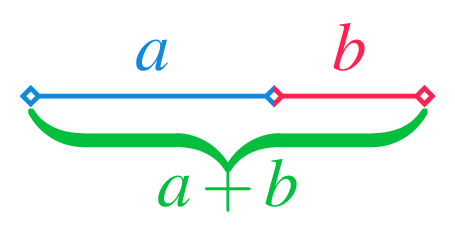
\includegraphics{././img/sucesiones/numero-aureo.png}

tal que \(\frac{a+b}{a}=\frac{a}{b}=\varphi\). A este número se le
conoce como
\href{https://es.wikipedia.org/wiki/N\%C3\%BAmero_\%C3\%A1ureo}{número
áureo} y es el número irracional
\(\varphi=\frac{1+\sqrt{5}}{2}=1.618033988749\ldots\)

Demostrar que este número es el límite de las siguientes sucesiones de
números reales.

\begin{enumerate}
\def\labelenumi{\alph{enumi}.}
\tightlist
\item
  \(x_1=1\) y \(x_{n+1}=1+\frac{1}{x_n}\) \(\forall n\in \mathbb{N}\)
\item
  \(x_1=1\) y \(x_{n+1}=\sqrt{1+x_n}\) \(\forall n\in\mathbb{N}\)
\end{enumerate}

\end{exercise}

\begin{tcolorbox}[enhanced jigsaw, leftrule=.75mm, rightrule=.15mm, colbacktitle=quarto-callout-tip-color!10!white, opacitybacktitle=0.6, bottomtitle=1mm, coltitle=black, colback=white, titlerule=0mm, left=2mm, arc=.35mm, breakable, colframe=quarto-callout-tip-color-frame, toprule=.15mm, toptitle=1mm, opacityback=0, title=\textcolor{quarto-callout-tip-color}{\faLightbulb}\hspace{0.5em}{Solución}, bottomrule=.15mm]

\begin{enumerate}
\def\labelenumi{\alph{enumi}.}
\item
  Veamos en primer lugar que la sucesión está acotada. De la definición
  resulta obvio que \(x_n\geq 1\) \(\forall n\in\mathbb{N}\). De esto se
  deduce que,
  \(\frac{1}{x_n}\leq 1 \Leftrightarrow 1+\frac{1}{x_n} \leq 2\)
  \(\forall n\in\mathbb{N}\). Así pues, \(1\leq x_n\leq 2\)
  \(\forall n\in\mathbb{N}\).

  Veamos ahora que la subsucesión de los términos impares
  \((y_n)_{n=1}^\infty = (x_{2n-1})_{n=1}^\infty\) converge. Para ello
  veremos que es creciente por inducción. \(y_1=1<y_2=1.5\). Supongamos
  que \(y_{n-1}<y_n\). Entonces,

  \begin{align*}
   y_{n+1} &= x_{2(n+1)-1} = x_{2n+1} = 1+\frac{1}{x_{2n}} \\ 
   &= 1+\frac{1}{1+\frac{1}{x_{2n-1}}} = 1+\frac{1}{1+\frac{1}{y_n}} \\ 
   &> 1+\frac{1}{1+\frac{1}{y_{n-1}}} = 1+\frac{1}{1+\frac{1}{x_{2n-3}}} \\
   &= 1+\frac{1}{x_{2n-2}} = x_{2n-1} = y_n.
   \end{align*}

  Como la subsucesión también está acotada, por el
  \href{https://aprendeconalf.es/analisis-manual/sucesiones.html\#thm-convergencia-monotona}{teorema
  de la convergencia de sucesiones monótonas} converge. Para calcular el
  límite, aprovechando la definición recursiva de la sucesión se tiene

  \[
   y = \lim_{n\to\infty}y_n = \lim_{n\to\infty}y_{n+1} = \lim_{n\to\infty}1+\frac{1}{1+\frac{1}{y_n}} = 1+\frac{1}{1+\frac{1}{y}}
   \]

  Resolviendo la ecuación se tiene

  \begin{align*}
   y=1+\frac{1}{1+\frac{1}{y}} &\Rightarrow y-1= \frac{1}{\frac{y+1}{y}} = \frac{y}{y+1} \\ 
   &\Rightarrow (y-1)(y+1) = y \\ 
   & \Rightarrow y^2-1 = y \Rightarrow y^2-y-1=0 \\ 
   &\Rightarrow y=\frac{1-\sqrt{5}}{2} \mbox{ o } y=\frac{1+\sqrt{5}}{2}.
   \end{align*}

  Como \(y=\frac{1-\sqrt{5}}{2}<0\) no puede ser al ser todos los
  términos de la sucesión positivos, se tiene que
  \(y=\frac{1+\sqrt{5}}{2}\).

  Del mismo modo se puede probar que la subsucesión de los términos
  pares \((z_n)_{n=1}^\infty = (x_{2n})_{n=1}^\infty\) también converge
  a \(\frac{1+\sqrt{5}}{2}\).

  Finalmente, se deja como ejercicio probar que si las subsucesiones de
  los términos pares e impares de una sucesión convergen al mismo
  límite, entonces la sucesión converge al mismo límite.
\item
  Veamos que la sucesión es creciente por inducción.
  \(x_1=1<\sqrt{2}=x_2\). Supongamos ahora que \(x_{n-1}<x_n\).
  Entonces, \(x_{n+1} = \sqrt{1+x_n} > \sqrt{1+x_{n-1}} = x_n\).

  Veamos ahora que \(2\) es una cota superior de la sucesión también por
  inducción. \(x_1 = 1 < 2\). Supongamos que \(x_n<2\). Entonces,
  \(x_{n+1}=\sqrt{1+x_n} < \sqrt{1+2} = \sqrt{3} < 2\).

  Así pues, según el
  \href{https://aprendeconalf.es/analisis-manual/sucesiones.html\#thm-convergencia-monotona}{teorema
  de la convergencia de sucesiones monótonas} la sucesión converge. Para
  calcular el límite, aprovechando la definición recursiva de la
  sucesión se tiene

  \[
   x = \lim_{n\to\infty}x_n = \lim_{n\to\infty}x_{n+1} = \lim_{n\to\infty}\sqrt{1+x_n} = \sqrt{1+x}
   \]

  Resolviendo la ecuación se tiene

  \begin{align*}
   x=\sqrt{1+x} &\Rightarrow x^2=1+x \Rightarrow x^2-x-1=0 \\ 
   &\Rightarrow x=\frac{1-\sqrt{5}}{2} \mbox{ o } x=\frac{1+\sqrt{5}}{2}.
   \end{align*}

  Como \(x=\frac{1-\sqrt{5}}{2}<0\) no puede ser al ser todos los
  términos de la sucesión positivos, se concluye que
  \(x=\frac{1+\sqrt{5}}{2}\).
\end{enumerate}

\end{tcolorbox}

\leavevmode\vadjust pre{\hypertarget{exr-condiciones-heredadas-limite}{}}%
\begin{exercise}[]\label{exr-condiciones-heredadas-limite}

Dada una sucesión de números reales tal que \(\lim_{n\to\infty}x_n=x\),
probar o refutar las siguientes proposiciones:

\begin{enumerate}
\def\labelenumi{\alph{enumi}.}
\tightlist
\item
  Si cada \(x_n\) es una cota superior de un conjunto \(A\), entonces
  \(x\) es también una cota superior de \(A\).
\item
  Si \(x_n\in\overline{(a,b)}\) \(\forall n\in\mathbb{N}\), entonces
  \(x\in\overline{(a,b)}\).
\item
  Si \(x_n\in\mathbb{Q}\) \(\forall n\in\mathbb{N}\), entonces
  \(x\in\mathbb{Q}\).
\end{enumerate}

\end{exercise}

\begin{tcolorbox}[enhanced jigsaw, leftrule=.75mm, rightrule=.15mm, colbacktitle=quarto-callout-tip-color!10!white, opacitybacktitle=0.6, bottomtitle=1mm, coltitle=black, colback=white, titlerule=0mm, left=2mm, arc=.35mm, breakable, colframe=quarto-callout-tip-color-frame, toprule=.15mm, toptitle=1mm, opacityback=0, title=\textcolor{quarto-callout-tip-color}{\faLightbulb}\hspace{0.5em}{Solución}, bottomrule=.15mm]

\begin{enumerate}
\def\labelenumi{\alph{enumi}.}
\item
  Si \(x_n\) es cota superior de \(A\) \(\forall n\in\mathbb{N}\), se
  tiene que para cualquier \(a\in A\), \(a\leq x_n\). Veamos que
  entonces que \(a\leq x\) por reducción al absurdo. Supongamos que
  existe \(a\in A\) tal que \(a\leq x_n\) \(\forall n\in\mathbb{N}\)
  pero \(a>x\). Como \(\lim_{n\to\infty}x_n = x\), se tiene que para
  \(\varepsilon=a-x>0\) existe \(k\in\mathbb{N}\) tal que
  \(|x_n-x|\leq a-x\) \(\forall n\geq k\), pero entonces también se
  cumple \[
  |x_n-x| = x_n-x < a-x \Rightarrow x_n < a,
  \] por lo que \(x_n\) no sería cota superior de \(A\), así que,
  necesariamente \(x\) tiene que ser cota superior de \(A\).
\item
  Como \(\overline{(a,b)}\) es un conjunto cerrado, para demostrar la
  proposición basta aplicar este
  \href{https://aprendeconalf.es/analisis-manual/sucesiones.html\#thm-sucesiones-conjuntos-cerrados}{teorema}.
\item
  Veamos que la proposición es falsa con un contraejemplo. La sucesión
  \(x_1=1\) y \(x_{n+1}=\frac{1}{1+x_n}\) \(\forall n=2,3,\ldots\) está
  formada por números racionales, sin embargo, su límite es el número
  irracional \(\varphi=\frac{1+\sqrt{5}}{2}=1.618033988749\ldots\) (ver
  Ejercicio~\ref{exr-numero-aureo}).
\end{enumerate}

\end{tcolorbox}

\leavevmode\vadjust pre{\hypertarget{exr-sucesion-intereses}{}}%
\begin{exercise}[]\label{exr-sucesion-intereses}

\(\star\) Una cuenta de ahorro ofrece el primer año un tipo de interés
\(x_1=0.5\%\) y los años sucesivos un interés
\(x_{n+1}=\frac{3}{2+x_n}\%\). Si se mantiene la cuenta abierta por un
periodo indefinido, ¿hacia donde tienden los tipos de interés?

\end{exercise}

\begin{tcolorbox}[enhanced jigsaw, leftrule=.75mm, rightrule=.15mm, colbacktitle=quarto-callout-tip-color!10!white, opacitybacktitle=0.6, bottomtitle=1mm, coltitle=black, colback=white, titlerule=0mm, left=2mm, arc=.35mm, breakable, colframe=quarto-callout-tip-color-frame, toprule=.15mm, toptitle=1mm, opacityback=0, title=\textcolor{quarto-callout-tip-color}{\faLightbulb}\hspace{0.5em}{Solución}, bottomrule=.15mm]

\begin{enumerate}
\def\labelenumi{\alph{enumi}.}
\item
  Veamos en primer lugar que la sucesión está acotada. De la definición
  resulta obvio que \(x_n\geq 0\) \(\forall n\in\mathbb{N}\) pues todos
  los términos son positivos. De esto se deduce que,
  \(\frac{3}{x+x_n}\leq \frac{3}{2}\) \(\forall n\in\mathbb{N}\). Así
  pues, \(0\leq x_n\leq \frac{3}{2}\) \(\forall n\in\mathbb{N}\).

  Veamos ahora que la subsucesión de los términos impares
  \((y_n)_{n=1}^\infty = (x_{2n-1})_{n=1}^\infty\) converge. Para ello
  veremos que es creciente por inducción. \(y_1=0.5<y_2=0.9375\).
  Supongamos que \(y_{n-1}<y_n\). Entonces,

  \begin{align*}
   y_{n+1} &= x_{2(n+1)-1} = x_{2n+1} = \frac{3}{2+x_{2n}} \\ 
   &= \frac{3}{2+\frac{3}{2+x_{2n-1}}} = \frac{3}{2+\frac{3}{2+y_n}} \\ 
   &> \frac{3}{2+\frac{3}{2+y_{n-1}}} = \frac{3}{2+\frac{3}{2+x_{2n-3}}} \\
   &= \frac{3}{2+x_{2n-2}} = x_{2n-1} = y_n.
   \end{align*}

  Como la subsucesión también está acotada, por el
  \href{https://aprendeconalf.es/analisis-manual/sucesiones.html\#thm-convergencia-monotona}{teorema
  de la convergencia de sucesiones monótonas} converge. Para calcular el
  límite, aprovechando la definición recursiva de la sucesión se tiene

  \[
   y = \lim_{n\to\infty}y_n = \lim_{n\to\infty}y_{n+1} = \lim_{n\to\infty}\frac{3}{2+\frac{3}{2+y_n}} = \frac{3}{2+\frac{3}{2+y}}
   \]

  Resolviendo la ecuación se tiene

  \begin{align*}
   y=\frac{3}{2+\frac{3}{2+y}} &\Rightarrow y= \frac{3}{\frac{(4+2y)+3}{2+y}} = \frac{3(2+y)}{2y+7} \\ 
   &\Rightarrow y(2y+7) = 3y+6 \\ 
   & \Rightarrow 2y^2+4y-6 = 0\\ 
   &\Rightarrow y=-3 \mbox{ o } y=1.
   \end{align*}

  Como \(y=-3\) no puede ser al ser todos los términos de la sucesión
  positivos, se tiene que \(y=1\).

  Del mismo modo se puede probar que la subsucesión de los términos
  pares \((z_n)_{n=1}^\infty = (x_{2n})_{n=1}^\infty\) también converge
  a \(1\).

  Finalmente, como las subsucesiones de los términos pares e impares de
  una sucesión convergen al mismo límite, entonces la sucesión converge
  al mismo límite.
\end{enumerate}

\end{tcolorbox}

\leavevmode\vadjust pre{\hypertarget{exr-sucesiones-cauchy}{}}%
\begin{exercise}[]\label{exr-sucesiones-cauchy}

Determinar cuáles de las siguientes sucesiones de números reales son de
Cauchy.

\begin{enumerate}
\def\labelenumi{\alph{enumi}.}
\item
  \(\left(\frac{(-1)^n}{n}\right)_{n=1}^\infty\)
\item
  \(\left(\frac{n}{n+1}\right)_{n=1}^\infty\)
\item
  \(\left(\frac{\operatorname{sen}(n)}{n}\right)_{n=1}^\infty\)
\item
  \((x_n)_{n=1}^\infty\) con \[
  x_n=
  \begin{cases}
  \frac{1}{n} & \mbox{si $n$ es par}\\
  1+\frac{1}{n} & \mbox{si $n$ es impar}
  \end{cases}
  \]
\end{enumerate}

\end{exercise}

\begin{tcolorbox}[enhanced jigsaw, leftrule=.75mm, rightrule=.15mm, colbacktitle=quarto-callout-tip-color!10!white, opacitybacktitle=0.6, bottomtitle=1mm, coltitle=black, colback=white, titlerule=0mm, left=2mm, arc=.35mm, breakable, colframe=quarto-callout-tip-color-frame, toprule=.15mm, toptitle=1mm, opacityback=0, title=\textcolor{quarto-callout-tip-color}{\faLightbulb}\hspace{0.5em}{Solución}, bottomrule=.15mm]

\begin{enumerate}
\def\labelenumi{\alph{enumi}.}
\item
  Es una sucesión de Cauchy ya que converge a 0, pues las subsucesiones
  de los términos pares e impares, convergen a 0 al ser monótonas y
  acotadas.
\item
  Es una sucesión de Cauchy ya que converge a 1, pues
\end{enumerate}

\begin{align*}
\lim_{n\to\infty} x_n &= \lim_{n\to\infty}\frac{n}{n+1} = \lim_{n\to\infty} \frac{1}{1+\frac{1}{n}}\\  
&= \frac{\lim_{n\to\infty} 1}{\lim_{n\to\infty} 1 + \lim_{n\to\infty}\frac{1}{n}} = \frac{1}{1} = 1.
\end{align*}

\begin{enumerate}
\def\labelenumi{\alph{enumi}.}
\setcounter{enumi}{2}
\tightlist
\item
  Es una sucesión de Cauchy ya que converge a 0. Para probarlo, dado
  \(\varepsilon>0\), por la propiedad arquimediana, existe
  \(k\in\mathbb{N}\) tal que \(\frac{2}{k}<\varepsilon\). Por tanto,
  para cualquier \(n,m\geq k\) se tiene
\end{enumerate}

\begin{align*}
|x_n-x_m| &= \left|\frac{\operatorname{sen}(n)}{n}-\frac{\operatorname{sen}(m)}{m}\right| \leq \left|\frac{\operatorname{sen}(n)}{n}\right|+\left|\frac{\operatorname{sen}(m)}{m}\right|\\  
& \leq \frac{1}{n}+\frac{1}{m}\leq \frac{1}{k}+\frac{1}{k} = \frac{2}{k} < \varepsilon.
\end{align*}

\begin{enumerate}
\def\labelenumi{\alph{enumi}.}
\setcounter{enumi}{3}
\tightlist
\item
  No es una sucesión de Cauchy, pues tomando \(\varepsilon=1/2\), para
  cualquier \(k\in\mathbb{N}\), si \(n\geq k\), entonces \(n\) o \(n+1\)
  debe ser impar, y suponiendo que es \(n+1\) (la otra suposición lleva
  a un razonamiento similar) se tiene
\end{enumerate}

\begin{align*}
|x_n-x_{n+1}| &\geq ||x_{n+1}|-|x_n|| =\left|\left(1+\frac{1}{n+1}\right)-\frac{1}{n}\right|\\ 
&=1-\frac{1}{n(n+1)}\geq 1 -\frac{1}{2} = \frac{1}{2}=\varepsilon.
\end{align*}

Por tanto, la sucesión no converge.

\end{tcolorbox}

\bookmarksetup{startatroot}

\hypertarget{luxedmites-de-funciones}{%
\chapter{Límites de funciones}\label{luxedmites-de-funciones}}

\leavevmode\vadjust pre{\hypertarget{exr-funcion-constante}{}}%
\begin{exercise}[]\label{exr-funcion-constante}

Sea \(f(x)=c\) una función constante. Demostrar que
\(\lim_{x\to a}f(x)=c\) \(\forall a\in\mathbb{R}\).

\end{exercise}

\begin{tcolorbox}[enhanced jigsaw, leftrule=.75mm, rightrule=.15mm, colbacktitle=quarto-callout-tip-color!10!white, opacitybacktitle=0.6, bottomtitle=1mm, coltitle=black, colback=white, titlerule=0mm, left=2mm, arc=.35mm, breakable, colframe=quarto-callout-tip-color-frame, toprule=.15mm, toptitle=1mm, opacityback=0, title=\textcolor{quarto-callout-tip-color}{\faLightbulb}\hspace{0.5em}{Solución}, bottomrule=.15mm]

Para cualquier \(\varepsilon>0\) se puede tomar \(\delta = 1\) tal que
si \(|x-a|<\delta=1\), entonces \(|f(x)-c| = |c-c|=0<\varepsilon\).

\end{tcolorbox}

\leavevmode\vadjust pre{\hypertarget{exr-definicion-limite}{}}%
\begin{exercise}[]\label{exr-definicion-limite}

\(\star\) Dada la función \(f(x)=4x-10\), demostrar usando la definición
de límite que \(\lim_{x\to 3}f(x)=2\).

\end{exercise}

\begin{tcolorbox}[enhanced jigsaw, leftrule=.75mm, rightrule=.15mm, colbacktitle=quarto-callout-tip-color!10!white, opacitybacktitle=0.6, bottomtitle=1mm, coltitle=black, colback=white, titlerule=0mm, left=2mm, arc=.35mm, breakable, colframe=quarto-callout-tip-color-frame, toprule=.15mm, toptitle=1mm, opacityback=0, title=\textcolor{quarto-callout-tip-color}{\faLightbulb}\hspace{0.5em}{Solución}, bottomrule=.15mm]

Para cualquier \(\varepsilon>0\) se puede tomar
\(\delta = \frac{\varepsilon}{4}\) tal que si
\(|x-3|<\delta=\frac{\varepsilon}{4}\), entonces

\[
|f(x)-2| = |4x-10-2|= |4x-12| = 4|x-3|<4\frac{\varepsilon}{4} =\varepsilon.
\]

\end{tcolorbox}

\leavevmode\vadjust pre{\hypertarget{exr-limite-criterio-sucesiones}{}}%
\begin{exercise}[]\label{exr-limite-criterio-sucesiones}

\(\star\) Dada la función \(f(x)=\frac{|x|}{x}\), usar el criterio de
las sucesiones para demostrar que no existe el límite de \(f\) en \(0\).

\end{exercise}

\begin{tcolorbox}[enhanced jigsaw, leftrule=.75mm, rightrule=.15mm, colbacktitle=quarto-callout-tip-color!10!white, opacitybacktitle=0.6, bottomtitle=1mm, coltitle=black, colback=white, titlerule=0mm, left=2mm, arc=.35mm, breakable, colframe=quarto-callout-tip-color-frame, toprule=.15mm, toptitle=1mm, opacityback=0, title=\textcolor{quarto-callout-tip-color}{\faLightbulb}\hspace{0.5em}{Solución}, bottomrule=.15mm]

Tomando las sucesión \(\left(\frac{-1}{n}\right)_{n=1}^\infty\) que
converge a \(0\), se tiene

\[
\lim_{n\to\infty}f\left(\frac{-1}{n}\right)=\lim_{n\to\infty}\frac{|-1/n|}{-1/n} = -1.
\]

Y tomando la sucesión \(\left(\frac{1}{n}\right)_{n=1}^\infty\) que
también converge a \(0\), se tiene

\[
\lim_{n\to\infty}f\left(\frac{1}{n}\right)=\lim_{n\to\infty}\frac{|1/n|}{1/n} = 1.
\]

Por tanto, por el criterio de las sucesiones convergentes, no existe el
límite de \(f\) en \(0\).

\end{tcolorbox}

\leavevmode\vadjust pre{\hypertarget{exr-limite-funcion-Dirichlet}{}}%
\begin{exercise}[]\label{exr-limite-funcion-Dirichlet}

La función \(f:\mathbb{R}\to \mathbb{R}\) dada por

\[
f(x)=\begin{cases}
1, & \mbox{si } x\in\mathbb{Q},\\ 
0, & \mbox{si } x\not\in \mathbb{Q}
\end{cases}
\] se conoce como la \emph{función de Dirichlet}. Demostrar que no
existe el límite de \(f\) en cualquier número real.

\end{exercise}

\begin{tcolorbox}[enhanced jigsaw, leftrule=.75mm, rightrule=.15mm, colbacktitle=quarto-callout-tip-color!10!white, opacitybacktitle=0.6, bottomtitle=1mm, coltitle=black, colback=white, titlerule=0mm, left=2mm, arc=.35mm, breakable, colframe=quarto-callout-tip-color-frame, toprule=.15mm, toptitle=1mm, opacityback=0, title=\textcolor{quarto-callout-tip-color}{\faLightbulb}\hspace{0.5em}{Solución}, bottomrule=.15mm]

Tomemos cualquier \(a\in\mathbb{R}\) y sea \((x_n)_{n=1}^\infty\) una
sucesión de números racionales que converja a \(a\). Entonces la
sucesión \((f(x_n))_{n=1}^\infty = (1)_{n=1}^\infty\) que converge a
\(1\). Por otro lado, sea \((y_n)_{n=1}^\infty\) una sucesión de números
irracionales que converja a \(a\). Entonces la sucesión
\((f(y_n))_{n=1}^\infty = (0)_{n=1}^\infty\) que converge a \(0\). Por
tanto, por el criterio de la sucesiones convergentes no existe el límite
de \(f\) en \(a\).

\end{tcolorbox}

\leavevmode\vadjust pre{\hypertarget{exr-limite-coseno}{}}%
\begin{exercise}[]\label{exr-limite-coseno}

\(\star\) Demostrar que no existe
\(\lim_{x\to 0}\cos\left(\frac{1}{x}\right)\).

\end{exercise}

\begin{tcolorbox}[enhanced jigsaw, leftrule=.75mm, rightrule=.15mm, colbacktitle=quarto-callout-tip-color!10!white, opacitybacktitle=0.6, bottomtitle=1mm, coltitle=black, colback=white, titlerule=0mm, left=2mm, arc=.35mm, breakable, colframe=quarto-callout-tip-color-frame, toprule=.15mm, toptitle=1mm, opacityback=0, title=\textcolor{quarto-callout-tip-color}{\faLightbulb}\hspace{0.5em}{Solución}, bottomrule=.15mm]

Tomando la sucesión \(\left(\frac{1}{(2n-1)\pi/2}\right)_{n=1}^\infty\)
que converge a \(0\), se tiene que

\[
\lim_{n\to\infty}\cos\left(\frac{1}{\frac{1}{(2n+1)\pi/2}}\right) = \lim_{n\to\infty
}\cos((2n-1)\pi/2) = 0.
\]

Y tomando la sucesión \(\left(\frac{1}{2n\pi}\right)_{n=1}^\infty\), que
también converge a \(0\), se tiene que

\[
\lim_{n\to\infty}\cos\left(\frac{1}{\frac{1}{2n\pi}}\right) = \lim_{n\to\infty
}\cos(2n\pi) = 1.
\]

Por tanto, por el criterio de las sucesiones convergentes, no existe el
límite de \(\cos\left(\frac{1}{x}\right)\) en \(0\).

\end{tcolorbox}

\leavevmode\vadjust pre{\hypertarget{exr-limite-polinomios}{}}%
\begin{exercise}[]\label{exr-limite-polinomios}

Dado un polinomio \(p(x)\), demostrar que \(\lim_{x\to a}p(x)=p(a)\)
\(\forall a\in\mathbb{R}\).

\end{exercise}

\begin{tcolorbox}[enhanced jigsaw, leftrule=.75mm, rightrule=.15mm, colbacktitle=quarto-callout-tip-color!10!white, opacitybacktitle=0.6, bottomtitle=1mm, coltitle=black, colback=white, titlerule=0mm, left=2mm, arc=.35mm, breakable, colframe=quarto-callout-tip-color-frame, toprule=.15mm, toptitle=1mm, opacityback=0, title=\textcolor{quarto-callout-tip-color}{\faLightbulb}\hspace{0.5em}{Solución}, bottomrule=.15mm]

Sea \(p(x)=a_0+a_1x+a_2x^2+\cdots+a_nx^n\), entonces, por el álgebra de
límites se tiene,

\begin{align*}
\lim_{x\to a}p(x) &= \lim_{x\to a} a_0+a_1x+a_2x^2+\cdots+a_nx^n\\ 
& = \lim_{x\to a} a_0 + \lim_{x\to a} a_1x +\lim_{x\to a} a_2x^2 + \cdots + \lim_{x\to a}a_nx^2 \\ 
&= a_0 + a_1 \lim_{x\to a} x + a_2\lim_{x\to a}x^2 + \cdots + a_n\lim_{x\to a}x^n\\ 
& = a_0+a_1a+a_2a^2+\cdots+a_na^n = p(a)
\end{align*}

\end{tcolorbox}

\leavevmode\vadjust pre{\hypertarget{exr-limite-funciones-racionales}{}}%
\begin{exercise}[]\label{exr-limite-funciones-racionales}

Dada una función racional \(f(x)=\frac{p(x)}{q(x)}\)
\(\forall x\in\mathbb{R}\) tal que \(q(x)\neq 0\), demostrar que
\(\lim_{x\to a}f(x)=f(a)\) \(\forall a\in\mathbb{R}\) tal que
\(q(a)\neq 0\).

\end{exercise}

\begin{tcolorbox}[enhanced jigsaw, leftrule=.75mm, rightrule=.15mm, colbacktitle=quarto-callout-tip-color!10!white, opacitybacktitle=0.6, bottomtitle=1mm, coltitle=black, colback=white, titlerule=0mm, left=2mm, arc=.35mm, breakable, colframe=quarto-callout-tip-color-frame, toprule=.15mm, toptitle=1mm, opacityback=0, title=\textcolor{quarto-callout-tip-color}{\faLightbulb}\hspace{0.5em}{Solución}, bottomrule=.15mm]

Sea \(f(x)=\frac{p(x)}{q(x)}\) con \(p(x)\) y \(q(x)\) dos polinomios.
Entonces, por el ejercicio anterior y el álgebra de límites se tiene que

\begin{align*}
\lim_{x\to a}f(x) &= \lim_{x\to a} \frac{p(x)}{q(x)} = \frac{\lim_{x\to a} p(x)}{\lim_{x\to a}q(x)} = \frac{p(a)}{q(a)}=f(a).
\end{align*}

\end{tcolorbox}

\leavevmode\vadjust pre{\hypertarget{exr-limite-emparedado}{}}%
\begin{exercise}[]\label{exr-limite-emparedado}

\(\star\) Demostrar, haciendo uso del
\href{https://aprendeconalf.es/analisis-manual/limites.html\#thm-compresión-funciones}{teorema
de compresión de funciones} que
\(\lim_{x\to 0}\frac{1-\cos(x)}{x} = 0\).

\end{exercise}

\begin{tcolorbox}[enhanced jigsaw, leftrule=.75mm, rightrule=.15mm, colbacktitle=quarto-callout-tip-color!10!white, opacitybacktitle=0.6, bottomtitle=1mm, coltitle=black, colback=white, titlerule=0mm, left=2mm, arc=.35mm, breakable, colframe=quarto-callout-tip-color-frame, toprule=.15mm, toptitle=1mm, opacityback=0, title=\textcolor{quarto-callout-tip-color}{\faLightbulb}\hspace{0.5em}{Solución}, bottomrule=.15mm]

\begin{align*}
\lim_{x\to 0}\frac{1-\cos(x)}{x} &= \lim_{x\to 0}\frac{(1-\cos(x))(1+\cos(x))}{x(1+\cos(x))} =  \lim_{x\to 0}\frac{1-\cos(x)^2}{x(1+\cos(x))}\\ 
&= \lim_{x\to 0}\frac{\operatorname{sen}(x)^2}{x(1+\cos(x))} = \lim_{x\to 0}\frac{\operatorname{sen}(x)}{x}\frac{\operatorname{sen}(x)}{1+\cos(x)} =\\ 
&= \lim_{x\to 0}\frac{\operatorname{sen}(x)}{x}\lim_{x\to 0}\frac{\operatorname{sen}(x)}{1+\cos(x)} =1\cdot 0 = 0.
\end{align*}

\end{tcolorbox}

\leavevmode\vadjust pre{\hypertarget{exr-limites-1}{}}%
\begin{exercise}[]\label{exr-limites-1}

\(\star\) Calcular los siguientes límites si existen:

\begin{enumerate}
\def\labelenumi{\alph{enumi}.}
\item
  \(\displaystyle \lim_{x\to 2} \dfrac{x^2+x-6}{x-2}\)
\item
  \(\displaystyle \lim_{x\to 1}\dfrac{x^3-3x+2}{x^4-4x+3}\)
\item
  \(\displaystyle \lim_{x\to 0}\dfrac{\operatorname{sen}(x+a)-\operatorname{sen}(a)}{x}\)
\item
  \(\displaystyle \lim_{x\to\infty}\dfrac{x^2-3x+2}{e^{2x}}\)
\item
  \(\displaystyle \lim_{x\to\infty}\dfrac{\log(x^2-1)}{x+2}\)
\item
  \(\displaystyle \lim_{x\to 1}\dfrac{\log(1/x)}{\operatorname{tg}(x+\dfrac{\pi}{2})}\)
\item
  \(\displaystyle \lim_{x\to a}\dfrac{x^n-a^n}{x-a}\quad n\in \mathbb{N}\)
\item
  \(\displaystyle \lim_{x\to 1}\dfrac{\sqrt[n]{x}-1}{\sqrt[m]{x}-1} \quad n,m \in \mathbb{Z}\)
\item
  \(\displaystyle \lim_{x\to 0}\dfrac{\operatorname{tg}(x)-\operatorname{sen}(x)}{x^3}\)
\end{enumerate}

\begin{enumerate}
\def\labelenumi{\alph{enumi}.}
\setcounter{enumi}{9}
\item
  \(\displaystyle \lim_{x\to \pi/4}\dfrac{\operatorname{sen}(x)-\cos(x)}{1-\operatorname{tg}(x)}\)
\item
  \(\displaystyle \lim_{x\to 0}x^2e^{1/x^2}\)
\item
  \(\displaystyle \lim_{x\to 0}\left(1+x\right)^{1/x}\)
\item
  \(\displaystyle \lim_{x\to \infty} \sqrt[x]{x^2}\)
\item
  \(\displaystyle \lim_{x\to 0}\left(\dfrac{1}{x}\right)^{\operatorname{tg}(x)}\)
\item
  \(\displaystyle \lim_{x\to 0}(\cos x)^{1/\operatorname{sen}(x)}\)
\item
  \(\displaystyle \lim_{x\to 0}\dfrac{6}{4+e^{-1/x}}\)
\item
  \(\displaystyle \lim_{x\to \infty}\left(\sqrt{x^2+x+1}-\sqrt{x^2-2x-1}\right)\).
\item
  \(\displaystyle \lim_{x\to \pi/2}\sec x-\operatorname{tg}(x)\)
\end{enumerate}

\end{exercise}

\begin{tcolorbox}[enhanced jigsaw, leftrule=.75mm, rightrule=.15mm, colbacktitle=quarto-callout-tip-color!10!white, opacitybacktitle=0.6, bottomtitle=1mm, coltitle=black, colback=white, titlerule=0mm, left=2mm, arc=.35mm, breakable, colframe=quarto-callout-tip-color-frame, toprule=.15mm, toptitle=1mm, opacityback=0, title=\textcolor{quarto-callout-tip-color}{\faLightbulb}\hspace{0.5em}{Solución}, bottomrule=.15mm]

\begin{enumerate}
\def\labelenumi{\alph{enumi}.}
\item
  \(\displaystyle \lim_{x\to 2} \dfrac{x^2+x-6}{x-2} = \lim_{x\to 2} \dfrac{(x+3)(x-2)}{x-2} = \lim_{x\to 2} \frac{x+3}{1}=5\).
\item
  \begin{align*}
   \lim_{x\to 1}\dfrac{x^3-3x+2}{x^4-4x+3} &= \lim_{x\to 1}\dfrac{(x-1)^2(x+2)}{(x-1)^2(x^2+2x+3)}\\  
   &= \lim_{x\to 1}\dfrac{(x+2)}{(x^2+2x+3)}= \frac{3}{6}=\frac{1}{2}.
   \end{align*}
\item
  Aplicando la propiedad trigonométrica
  \(\operatorname{sen}(x+a)=\operatorname{sen}(x)\cos(a)+\cos(x)\operatorname{sen}(a)\),
  se tiene

  \begin{align*}
   \lim_{x\to 0}\frac{\operatorname{sen}(x+a)-\operatorname{sen}(a)}{x} &= \lim_{x\to 0}\frac{\operatorname{sen}(x)\cos(a)+\cos(x)\operatorname{sen}(a)-\operatorname{sen}(a)}{x} \\ 
   &= \lim_{x\to 0}\frac{\operatorname{sen}(x)\cos(a)-\operatorname{sen}(a)(1-\cos(x))}{x} \\ 
   &= \cos(a)\lim_{x\to 0}\frac{\operatorname{sen}(x)}{x}-\operatorname{sen}(a)\lim_{x\to 0}\frac{1-\cos(x)}{x}\\
   & = \cos(a)\cdot 1-\operatorname{sen}(a)\cdot 0= \cos(a).
   \end{align*}
\item
  Como \(x<e^x\) \(\forall x>0\), se tiene que

  \[
   0<\frac{x}{2}<e^{x/2} \Rightarrow 0< x < 2e^{x/2} \Rightarrow  0< \frac{x}{e^{2x}} < \frac{2e^{x/2}}{e^{2x}} = \frac{2}{e^{3x/2}},\]

  de modo que, como \(\lim_{x\to\infty}\frac{2}{e^{3x/2}}=0\), aplicando
  el teorema de compresión de funciones se tiene que
  \(\lim_{x\to\infty} \frac{x}{e^{2x}}=0\).

  Usando este resultado se tiene,

  \[\lim_{x\to\infty}\dfrac{x^2-3x+2}{e^{2x}} = \lim_{x\to\infty}\dfrac{x^2}{e^{2x}}-3\lim_{x\to\infty} \frac{x}{e^{2x}} + \lim_{x\to\infty} \frac{2}{e^{2x}} = 0.
   \]
\item
  Cuando \(x\to\infty\),
  \(\frac{\log(x^2-1)}{x+2}\to \frac{\infty}{\infty}\) que es
  indeterminado. Aplicando la regla de L'Hôpital se tiene,

  \[
   \lim_{x\to\infty}\dfrac{\log(x^2-1)}{x+2} =\lim_{x\to\infty}\frac{1/x}{1} =0.
   \]
\item
  \(\displaystyle \lim_{x\to 1}\frac{\log(1/x)}{\operatorname{tg}(x+\frac{\pi}{2})} = \frac{\lim_{x\to 1}\log(1/x)}{\lim_{x\to 1}\operatorname{tg}(x+\frac{\pi}{2})} = \frac{\log(1)}{\operatorname{tg}(1+\frac{\pi}{2})}=0\)
\item
  \(x^n-a^n = (x-a)(x^{n-1}+ax^{n-2}+a^2x^{n-3}+\cdots + a^{n-2}x+a^{n-1}\)
  \(\forall n\in\mathbb{N}\), \(n\geq 2\). Así pues,

  \begin{align*}
   \lim_{x\to a}\dfrac{x^n-a^n}{x-a} &= \lim_{x\to a}\frac{(x-a)(x^{n-1}+ax^{n-2}+\cdots + a^{n-2}x+a^{n-1}}{x-a} \\ 
   &= \lim_{x\to a} x^{n-1}+ax^{n-2}+\cdots + a^{n-2}x+a^{n-1}\\  
   &= a^{n-1}+\stackrel{n}{\dots}+a^{n-1} = na^{n-1}
   \end{align*}
\item
  Cuando \(x\to 1\)
  \(\frac{\sqrt[n]{x}-1}{\sqrt[m]{x}-1}\to \frac{0}{0}\) que es
  indeterminado. Aplicando la regla de L'Hôpital se tiene

  \begin{align*}
   \lim_{x\to 1}\frac{\sqrt[n]{x}-1}{\sqrt[m]{x}-1} &= \lim_{x\to 1}\frac{x^{1/n}-1}{x^{1/m}-1} = \lim_{x\to 1}\frac{\frac{1}{n}x^{1/n-1}}{\frac{1}{m}x^{1/m-1}}\\  
   &= \lim_{x\to 1}\frac{mx^{1/n-1}}{nx^{1/m-1}} = \frac{m}{n}.
   \end{align*}
\item
  Como \(\operatorname{sen}(x)\approx\operatorname{tg}(x)\approx x\)
  cuando \(x\to 0\), se tiene

  \[
   \lim_{x\to 0}\frac{\operatorname{tg}(x)-\operatorname{sen}(x)}{x^3} = \lim_{x\to 0}\frac{x-x}{x^3} = \lim_{x\to 0}\frac{0}{x^3} = 0.
   \]
\item
  Aplicando propiedades trigonométricas se tiene

  \begin{align*}
   \lim_{x\to \pi/4}\frac{\operatorname{sen}(x)-\cos(x)}{1-\operatorname{tg}(x)} &= \lim_{x\to \pi/4}\frac{\operatorname{sen}(x)-\cos x}{1-\frac{\operatorname{sen}(x)}{\cos(x)}}\\ 
   & = \lim_{x\to \pi/4}\frac{\operatorname{sen}(x)-\cos x}{\frac{\cos(x)-\operatorname{sen}(x)}{\cos(x)}}\\ 
   & = \lim_{x\to \pi/4} -\cos(x) = \frac{-\sqrt{2}}{2}.
   \end{align*}
\item
  Cuando \(x\to 0\), \(x^2e^{1/x^2}\to 0\cdot \infty\), que es
  indeterminado. Transformando la indeterminación en una de tipo
  cociente y aplicando la regla de L'Hôpital se tiene

  \begin{align*}
   \lim_{x\to 0}x^2e^{1/x^2} &= \lim_{x\to 0}\frac{e^{1/x^2}}{1/x^2} = \lim_{x\to 0}\frac{e^{1/x^2}\frac{-2}{x^3}}{-2/x^3} = \lim_{x\to 0} e^{1/x^2} =\infty.
   \end{align*}
\item
  Cuando \(x\to 0\), \(\ln(1+x)\approx x\), de manera que

  \begin{align*}
   \lim_{x\to 0}\left(1+x\right)^{1/x} &= \lim_{x\to 0}e^{\ln(\left(1+x\right)^{1/x})} = e^{\lim_{x\to 0}\frac{\ln(1+x)}{x}}\\  
   &= e^{\lim_{x\to 0}\frac{x}{x}} = e^{\lim_{x\to 0}1} = e^1 = e.
   \end{align*}
\item
  Cuando \(x\to\infty\) \(\sqrt[x]{x^2}=x^{2/x}\to \infty^0\), que es
  intedeterminado. Transformando la indeterminación en una de tipo
  cociente y aplicando la regla de L'Hôpital, se tiene

  \begin{align*}
   \lim_{x\to \infty} \sqrt[x]{x^2} 
   &= \lim_{x\to \infty} x^{2/x} = \lim_{x\to \infty} e^{\ln(x^{2/x})}\\
   & = e^{\lim_{x\to \infty} \frac{2\ln(x)}{x}} = e^{\lim_{x\to \infty} \frac{\frac{2}{x}}{1}} = 1.
   \end{align*}
\item
  \(\displaystyle \lim_{x\to 0}\left(\dfrac{1}{x}\right)^{\operatorname{tg}(x)}\)
\item
  \(\displaystyle \lim_{x\to 0}(\cos x)^{1/\operatorname{sen}(x)}\)
\item
  \(\displaystyle \lim_{x\to 0}\dfrac{6}{4+e^{-1/x}}\)
\item
  \(\displaystyle \lim_{x\to \infty}\left(\sqrt{x^2+x+1}-\sqrt{x^2-2x-1}\right)\).
\item
  \(\displaystyle \lim_{x\to \pi/2}\sec x-\operatorname{tg}(x)\)
\end{enumerate}

\end{tcolorbox}

\leavevmode\vadjust pre{\hypertarget{exr-ejemplos-limites-laterales}{}}%
\begin{exercise}[]\label{exr-ejemplos-limites-laterales}

\(\star\) Dar ejemplo de funciones que cumplan las siguientes
condiciones:

\begin{enumerate}
\def\labelenumi{\alph{enumi}.}
\item
  \(\lim_{x\to 0}f(x)=+\infty\) y \(\lim_{x\to \infty}f(x)=0\).
\item
  \(\lim_{x\to 3^+}f(x)=+\infty\), \(\lim_{x\to 3^-}f(x)=-\infty\) y
  \(\lim_{x\to \infty}f(x)=1\).
\item
  \(\lim_{x\to 0^+}f(x)=+\infty\) y \(\lim_{x\to \infty}f(x)=-\infty\)
\end{enumerate}

\end{exercise}

\begin{tcolorbox}[enhanced jigsaw, leftrule=.75mm, rightrule=.15mm, colbacktitle=quarto-callout-tip-color!10!white, opacitybacktitle=0.6, bottomtitle=1mm, coltitle=black, colback=white, titlerule=0mm, left=2mm, arc=.35mm, breakable, colframe=quarto-callout-tip-color-frame, toprule=.15mm, toptitle=1mm, opacityback=0, title=\textcolor{quarto-callout-tip-color}{\faLightbulb}\hspace{0.5em}{Solución}, bottomrule=.15mm]

\begin{enumerate}
\def\labelenumi{\alph{enumi}.}
\item
  \(f(x)=\frac{1}{x^2}\).
\item
  \(g(x)=\frac{x}{x-3}\).
\item
  \(h(x)=-\ln(x)\).
\end{enumerate}

\end{tcolorbox}

\leavevmode\vadjust pre{\hypertarget{exr-limite-laterales}{}}%
\begin{exercise}[]\label{exr-limite-laterales}

\(\star\) Sea \(g(x)=e^{1/x}\) \(\forall x\neq 0\). Demostrar que no
existe el límite de \(g\) en \(0\).

\end{exercise}

\begin{tcolorbox}[enhanced jigsaw, leftrule=.75mm, rightrule=.15mm, colbacktitle=quarto-callout-tip-color!10!white, opacitybacktitle=0.6, bottomtitle=1mm, coltitle=black, colback=white, titlerule=0mm, left=2mm, arc=.35mm, breakable, colframe=quarto-callout-tip-color-frame, toprule=.15mm, toptitle=1mm, opacityback=0, title=\textcolor{quarto-callout-tip-color}{\faLightbulb}\hspace{0.5em}{Solución}, bottomrule=.15mm]

Basta con probar que el límite lateral por la derecha no existe. Para
ello, tomando la sucesión de términos positivos
\(\left(\frac{1}{n}\right)_1^\infty\) que converge a \(0\), se tiene que

\[
\lim_{n\to\infty}g\left(\frac{1}{n}\right) = \lim_{n\to\infty}e^{\frac{1}{1/n}} =  \lim_{n\to\infty}e^n = \infty.
\] Así pues, según el criterio de las sucesiones convergentes, no existe
el límite por la derecha de \(g\) en \(0\), y por tanto tampoco existe
el límite.

\end{tcolorbox}

\leavevmode\vadjust pre{\hypertarget{exr-limites-laterales}{}}%
\begin{exercise}[]\label{exr-limites-laterales}

Dada la función

\[
f(x)=\begin{cases}
x^2, \mbox{si } x\leq 1,\\ 
ax-1, \mbox{si } x>1
\end{cases}
\]

con \(a\in\mathbb{R}\). ¿Para que valor de \(a\) existe el límite de
\(f\) en \(1\)?

\end{exercise}

\begin{tcolorbox}[enhanced jigsaw, leftrule=.75mm, rightrule=.15mm, colbacktitle=quarto-callout-tip-color!10!white, opacitybacktitle=0.6, bottomtitle=1mm, coltitle=black, colback=white, titlerule=0mm, left=2mm, arc=.35mm, breakable, colframe=quarto-callout-tip-color-frame, toprule=.15mm, toptitle=1mm, opacityback=0, title=\textcolor{quarto-callout-tip-color}{\faLightbulb}\hspace{0.5em}{Solución}, bottomrule=.15mm]

Los límtes laterales en 1 valen

\(\lim_{x\to 1^-} f(x) = \lim_{x\to 1^-} x^2 = 1^2 = 1.\)
\(\lim_{x\to 1^+} f(x) = \lim_{x\to 1^+} ax-1 = a-1.\)

Para que exista el límite de \(f\) en \(1\) debe ser
\(\lim_{x\to 1^-}f(x)=\lim_{x\to 1^+}f(x)\), es decir, \(1=a-1\), luego
debe ser \(a=2\).

\end{tcolorbox}

\leavevmode\vadjust pre{\hypertarget{exr-limites-laterales-2}{}}%
\begin{exercise}[]\label{exr-limites-laterales-2}

\(\star\) Calcular los límites laterales de la función
\(f(x)=\dfrac{1}{1+e^{\frac{1}{1-x}}}\) en el punto \(x=1\). ¿Existe el
límite en ese punto?

\end{exercise}

\begin{tcolorbox}[enhanced jigsaw, leftrule=.75mm, rightrule=.15mm, colbacktitle=quarto-callout-tip-color!10!white, opacitybacktitle=0.6, bottomtitle=1mm, coltitle=black, colback=white, titlerule=0mm, left=2mm, arc=.35mm, breakable, colframe=quarto-callout-tip-color-frame, toprule=.15mm, toptitle=1mm, opacityback=0, title=\textcolor{quarto-callout-tip-color}{\faLightbulb}\hspace{0.5em}{Solución}, bottomrule=.15mm]

\begin{align*}
\lim_{x\to 1^-}f(x) &= \lim_{x\to 1^-} \frac{1}{1+e^{\frac{1}{1-x}}} = \frac{1}{1+\lim_{x\to 1^-}e^\frac{1}{1-x}}\\ 
&= \frac{1}{1+e^{\lim_{x\to 1^-}\frac{1}{1-x}}} =  \frac{1}{1+e^\infty} = \frac{1}{1+\infty} = 0.
\end{align*}

\begin{align*}
\lim_{x\to 1^+}f(x) &= \lim_{x\to 1^+} \frac{1}{1+e^{\frac{1}{1-x}}} = \frac{1}{1+\lim_{x\to 1^+}e^\frac{1}{1-x}}\\ 
&= \frac{1}{1+e^{\lim_{x\to 1^+}\frac{1}{1-x}}} =  \frac{1}{1+e^{-\infty}} = \frac{1}{1+0} = 1.
\end{align*}

Como los límites laterales son distintos, no existe el límite de \(f\)
en \(1\).

\end{tcolorbox}

\leavevmode\vadjust pre{\hypertarget{exr-asintotas}{}}%
\begin{exercise}[]\label{exr-asintotas}

\(\star\) Calcular las asíntotas de las siguientes funciones:

\begin{enumerate}
\def\labelenumi{\alph{enumi}.}
\item
  \(f(x)=(1-x)e^x\)
\item
  \(g(x)=xe^{1/x}\)
\item
  \(h(x)=2x^2-\ln(x)\)
\end{enumerate}

\begin{enumerate}
\def\labelenumi{\alph{enumi}.}
\setcounter{enumi}{3}
\item
  \(i(x)=\log(x^2+3x+2)\)
\item
  \(j(x)=\dfrac{x^3}{(x+1)^2}\)
\item
  \(k(x)=\cos x-\log(\cos x)\)
\end{enumerate}

\end{exercise}

\begin{tcolorbox}[enhanced jigsaw, leftrule=.75mm, rightrule=.15mm, colbacktitle=quarto-callout-tip-color!10!white, opacitybacktitle=0.6, bottomtitle=1mm, coltitle=black, colback=white, titlerule=0mm, left=2mm, arc=.35mm, breakable, colframe=quarto-callout-tip-color-frame, toprule=.15mm, toptitle=1mm, opacityback=0, title=\textcolor{quarto-callout-tip-color}{\faLightbulb}\hspace{0.5em}{Solución}, bottomrule=.15mm]

\begin{enumerate}
\def\labelenumi{\alph{enumi}.}
\item
  \(f\) está definida en \(\mathbb{R}\), así que no tiene asíntotas
  verticales.

  Para ver si \(f\) tiene asíntotas horizontales estudiamos los límites
  en el infinito. Cuando \(x\to -\infty\) \((1-x)e^x\to -\infty\cdot 0\)
  que es indeterminado. Transformando la indeterminación en una de tipo
  cociente

  \begin{align*}
   \lim_{x\to -\infty}(1-x)e^x &= \lim_{x\to -\infty}\frac{1-x}{e^-x} = \lim_{x\to -\infty}\frac{1}{e^{-x}}- \lim_{x\to -\infty} \frac{-x}{e^{-x}}\\ 
   &= 0 -\lim_{x\to -\infty}\frac{-x}{e^{-x}}.
   \end{align*}

  Por otro lado \(\forall x<0\) se cumple que \(e^{-x}\geq x^2\)
  \(0\leq \frac{-x}{e^{-x}}\leq \frac{-x}{x^2}=\frac{1}{x}\), y como
  \(\lim_{x\to -\infty}\frac{-1}{x}=0\), por el teorema de compresión de
  funciones se tiene que \(\lim_{x\to -\infty}\frac{-x}{e^{-x}} = 0\).

  Así pues, \(y=0\) es una asíntota horizontal en \(-\infty\).

  Por otro lado,
  \(\lim_{x\to \infty}(1-x)e^x = -\infty*\infty = -\infty\), de modo que
  no hay asíntota horizontal en \(\infty\).

  Finalmente para ver si \(f\) tiene asíntotas oblicuas, estudiamos
  estudiamos el límite de \(f(x)/x\) en \(\infty\) (en \(-\infty\) no
  puede haber asíntota oblicua porque existe una horizontal).

  \[
   \lim_{x\to \infty}\frac{(1-x)e^x}{x} = \lim_{x\to \infty} \frac{1-x}{x}\lim_{x\to \infty}e^x = -1\cdot \infty = -\infty.
   \]

  Por tanto, tampoco existe asíntota oblicua en \(\infty\).
\item
  \(g\) está definida en \(\mathbb{R}\setminus \{0\}\), así que, el
  único punto donde pueden existir asíntotas verticales es \(x=0\).
  Calculando los límites laterales se tiene

  \begin{align*}
   \lim_{x\to 0^-} xe^{1/x} &= \lim_{x\to 0^-}x \lim_{x\to 0^-}e^{1/x} = 0\cdot e^-\infty = 0\cdot 0 = 0.\\ 
   \lim_{x\to 0^+} xe^{1/x} &= \lim_{x\to 0^+}\frac{e^{1/x}}{1/x} = \lim_{x\to 0^+}\frac{(e^{1/x})'}{(1/x)'} \tag{\small L'Hôpital}\\ 
   &= \lim_{x\to 0^+}\frac{e^{1/x}(1/x)'}{(1/x)'} = \lim_{x\to 0^+}e^{1/x} = \infty. 
   \end{align*}

  Por tanto, \(g\) tiene asíntota vertical \(x=0\) por la derecha, pero
  no por la izquierda.

  Para ver si \(g\) tiene asíntotas horizontales estudiamos los límites
  en el infinito.

  \begin{align*}
   \lim_{x\to -\infty}xe^{1/x} &= \lim_{x\to -\infty}x \lim_{x\to -\infty}e^{1/x} = \infty * 1 = \infty.\\ 
   \lim_{x\to \infty}xe^{1/x} &= \lim_{x\to \infty}x \lim_{x\to \infty}e^{1/x} = \infty * 1 = \infty.
   \end{align*}

  Así pues, ambos límites no existen y, por tanto, \(g\) no tiene
  asíntotas horizontales.

  Finalmente para ver si \(f\) tiene asíntotas oblicuas, estudiamos
  estudiamos el límite de \(f(x)/x\) en \(\pm\infty\).

  \[
   \lim_{x\to -\infty}\frac{xe^{1/x}}{x} = \lim_{x\to -\infty} e^{1/x} = e^0 =1.
   \]

  Luego, existe una asíntota oblicua en \(-\infty\) con pendiente \(1\).
  Para ver el término independiente de la asíntota calculamos el límite
  de \(f(x)-1\cdot x\) en \(-\infty\).

  \begin{align*}
   \lim_{x\to -\infty}xe^{1/x}-x &= \lim_{x\to -\infty} x(e^{1/x}-1) = \lim_{x\to -\infty} \frac{e^{1/x}-1}{1/x} \\ 
   &= \lim_{x\to -\infty} \frac{(e^{1/x}-1)'}{(1/x)'} \tag{\small L'Hôpital}\\ 
   &= \lim_{x\to -\infty} \frac{e^{1/x} (1/x)'}{(1/x)'} = \lim_{x\to -\infty} e^{1/x} = 1.
   \end{align*}

  Así pues, \(g\) tiene una asíntota oblicua \(y=x+1\) en \(-\infty\).
  Del mismo modo se puede probar que esta misma recta es asíntota
  oblicua en \(\infty\).
\item
  \(h(x)\) está definida en \(\mathbb{R}^+\), así que, el único punto
  donde pueden existir asíntotas verticales \(x=0\). Como \(h\) no está
  definida para \(x<0\), estudiaremos el límite por la derecha en \(0\).

  \[
   \lim_{x\to 0^+} 2x^2-\ln(x) = 0-\ln(0) = \infty
   \] Por tanto, \(h\) tiene una asíntota vertical \(x=0\) por la
  derecha, pero no por la izquierda.

  Para ver si \(g\) tiene asíntotas horizontales estudiamos el límite en
  el infinito (en \(-\infty\) no puede haber asíntota horizontal al no
  estar definida la función para \(x<0\)).

  \begin{align*}
   \lim_{x\to\infty} 2x^2-\ln(x) &= \lim_{x\to\infty}\ln(e^{2x^2-\ln(x)}) = \lim_{x\to \infty} \ln\left(\frac{e^{2x^2}}{e^{\ln(x)}}\right)\\ 
   &= \ln\left(\lim_{x\to \infty} \frac{e^{2x^2}}{x}\right) = \ln\left(\lim_{x\to \infty} \frac{(e^{2x^2})'}{x'}\right) \tag{L'Hôpital} \\ 
   &= \ln\left(\lim_{x\to \infty} \frac{e^{2x^2}4x}{1}\right) = \ln(\infty) = \infty.
   \end{align*}

  Por tanto, \(h\) no tiene asíntotas horizontales.

  Finalmente, veamos si existe asíntota oblicua en \(\infty\).

  \begin{align*}
   \lim_{x\to\infty} \frac{2x^2-\ln(x)}{x} &= \lim_{x\to \infty} 2x - \frac{\ln(x)}{x}\\ 
   & = \lim_{x\to \infty} 2x -\lim_{x\to \infty}\frac{\ln(x)}{x}\\ 
   &= \lim_{x\to \infty} 2x -\lim_{x\to \infty}\frac{(\ln(x))'}{x'} \tag{L'Hôpital}\\ 
   & = \lim_{x\to \infty} 2x -\lim_{x\to \infty}\frac{1}{x}= \infty-0=\infty.  
   \end{align*}

  Luego, \(h\) tampoco tiene asíntota oblicua en \(\infty\).
\end{enumerate}

\end{tcolorbox}

\leavevmode\vadjust pre{\hypertarget{exr-acuifero}{}}%
\begin{exercise}[]\label{exr-acuifero}

\(\star\) Mediante simulación por ordenador se ha podido cuantificar la
cantidad de agua almacenada en un acuífero en función del tiempo,
\(m(t)\), en millones de metros cúbicos, y el tiempo \(t\) en años
transcurridos desde el instante en el que se ha hecho la simulación,
teniendo en cuenta que la ecuación sólo tiene sentido para \(t>0\):

\[
m(t) = 10 + \frac{\sqrt{t}}{e^t}
\]

¿Qué cantidad de agua almacenada habrá en el acuífero asintóticamente?

\end{exercise}

\begin{tcolorbox}[enhanced jigsaw, leftrule=.75mm, rightrule=.15mm, colbacktitle=quarto-callout-tip-color!10!white, opacitybacktitle=0.6, bottomtitle=1mm, coltitle=black, colback=white, titlerule=0mm, left=2mm, arc=.35mm, breakable, colframe=quarto-callout-tip-color-frame, toprule=.15mm, toptitle=1mm, opacityback=0, title=\textcolor{quarto-callout-tip-color}{\faLightbulb}\hspace{0.5em}{Solución}, bottomrule=.15mm]

Cuando \$t\to\infty \(\frac{\sqrt{t}}{e^t}\to \frac{\infty}{\infty}\)
que es indeterminado. Aplicando la regla de L'Hôpital se tiene

\[
\lim_{t\to \infty} 10 + \frac{\sqrt{t}}{e^t} = 10 + \lim_{t\to \infty} \frac{\sqrt{t}}{e^t} = \\lim_{t\to \infty}\frac{1}{2\sqrt(t)e^t} = 10.
\]

Por tanto el volumen del lato tiende asintóticamente a 10 millones de
metros cúbicos.

\end{tcolorbox}

\leavevmode\vadjust pre{\hypertarget{exr-cosecha}{}}%
\begin{exercise}[]\label{exr-cosecha}

\(\star\) La cosecha de trigo de una plantación (en toneladas) depende
de la cantidad de abono \(x\) según la función
\(f(x)=T(1-\frac{1}{2}e^{-kx})\), donde \(T\) es la extensión del
terreno (en hectáreas) y \(k\) es la proporción de humedad. ¿Para qué
cantidad de abono se conseguiría una cosecha de \(T\) toneladas de
trigo?

\end{exercise}

\begin{tcolorbox}[enhanced jigsaw, leftrule=.75mm, rightrule=.15mm, colbacktitle=quarto-callout-tip-color!10!white, opacitybacktitle=0.6, bottomtitle=1mm, coltitle=black, colback=white, titlerule=0mm, left=2mm, arc=.35mm, breakable, colframe=quarto-callout-tip-color-frame, toprule=.15mm, toptitle=1mm, opacityback=0, title=\textcolor{quarto-callout-tip-color}{\faLightbulb}\hspace{0.5em}{Solución}, bottomrule=.15mm]

Como \(k>0\) se tiene \(\frac{1}{2}e^{-kx} = \frac{1}{2e^{kx}} < 1\)
\(\forall x>0\), de manera que \(f(x)<T\) \(\forall x>0\). Si calculamos
ahora el límite en infinito se tiene

\[\lim_{x\to \infty} T(1-\frac{1}{2}e^{-kx}) = T(1-\lim_{x\to \infty}\frac{1}{2e^{kx}}) = T(1-0) = T.
\]

De modo la cantidad de trigo cosechada tiene asintóticamente a \(T\),
pero al ser menor que \(T\), nunca llegará a valer \(T\).

\end{tcolorbox}

\leavevmode\vadjust pre{\hypertarget{exr-limites-funciones-acotadas}{}}%
\begin{exercise}[]\label{exr-limites-funciones-acotadas}

Sea \(f:(a,b)\to \mathbb{R}\) una función creciente. Demostrar lo
siguiente:

\begin{enumerate}
\def\labelenumi{\alph{enumi}.}
\tightlist
\item
  Si \(f\) está acotada superiormente, entonces existe
  \(\lim_{x\to b^-}f(x)\).
\item
  Si \(f\) no está acotada superiormente, entonces
  \(\lim_{x\to b^-}f(x)=\infty\).
\end{enumerate}

\end{exercise}

\leavevmode\vadjust pre{\hypertarget{exr-continuidad-coseno}{}}%
\begin{exercise}[]\label{exr-continuidad-coseno}

Demostrar que la función \(f(x)=\cos(x)\) es continua en todo
\(\mathbb{R}\).

\end{exercise}

\leavevmode\vadjust pre{\hypertarget{exr-discontinuidad-evitable}{}}%
\begin{exercise}[]\label{exr-discontinuidad-evitable}

¿Qué tipo de discontinuidad presenta la función
\(f(x)=x\cos\left(\frac{1}{x}\right)\) en \(x=0\)? Redefinir la función
para que sea continua en dicho punto.

\end{exercise}

\leavevmode\vadjust pre{\hypertarget{exr-clasificacion-dicontinuidades}{}}%
\begin{exercise}[]\label{exr-clasificacion-dicontinuidades}

Estudiar la continuidad de las siguientes funciones en los puntos que se
indican:

\begin{enumerate}
\def\labelenumi{\alph{enumi}.}
\item
  \(f(x)=\dfrac{e^x-1}{e^x+1}\), en el punto \(x=0\).
\item
  \[
  g(x)=
  \begin{cases}
  \frac{1+e^{1/x}}{1-e^{1/x}} & \mbox{si $x\neq 0$,} \\
  1 &  \mbox{si $x=0$,}
  \end{cases}
  \] en el punto \(x=0\).
\item
  \[
  h(x)=
  \begin{cases}
  x\operatorname{sen}\frac{\pi}{x} & \mbox{si $x\neq 0$,} \\
  0 & \mbox{si $x=0$,}
  \end{cases}
  \] en el punto \(x=0\).
\item
  \[
  i(x)=
  \begin{cases}
  \dfrac{1}{2^{1/x}} &  \mbox{si $x\neq 0$,} \\
  0 & \mbox{si $x=0$,}
  \end{cases}
  \] en el punto \(x=0\).
\end{enumerate}

\end{exercise}

\leavevmode\vadjust pre{\hypertarget{exr-clasificacion-dicontinuidades-2}{}}%
\begin{exercise}[]\label{exr-clasificacion-dicontinuidades-2}

Clasificar las discontinuidades de las siguientes funciones

\begin{enumerate}
\def\labelenumi{\alph{enumi}.}
\item
  \[
  f(x)=\frac{\frac{1}{x}-\frac{1}{x+1}}{\frac{3}{x-1}-\frac{1}{x}}.
  \]
\item
  \[
  g(x)=
  \begin{cases}
  \dfrac{\operatorname{sen}(x)}{x} & \text{si $x<0$,} \\ 
  e^{\frac{1}{x-1}} & \text{si $x\geq 0$.}
  \end{cases}
  \]
\end{enumerate}

\end{exercise}

\begin{tcolorbox}[enhanced jigsaw, leftrule=.75mm, rightrule=.15mm, colbacktitle=quarto-callout-tip-color!10!white, opacitybacktitle=0.6, bottomtitle=1mm, coltitle=black, colback=white, titlerule=0mm, left=2mm, arc=.35mm, breakable, colframe=quarto-callout-tip-color-frame, toprule=.15mm, toptitle=1mm, opacityback=0, title=\textcolor{quarto-callout-tip-color}{\faLightbulb}\hspace{0.5em}{Solución}, bottomrule=.15mm]

\begin{enumerate}
\def\labelenumi{\alph{enumi}.}
\item
  A simple vista, podemos ver que se trata de una función racional y
  estará definida en todo \(\mathbb{R}\) salvo en los puntos que anulen
  alguno de los denominadores. Dichos puntos son fáciles de obtener
  igualando a 0 los denominadores:

  \begin{align*}
   x &= 0 \\
   x+1 &= 0\Leftrightarrow x=-1 \\
   x-1 &= 0\Leftrightarrow x=1 \\
   \frac{3}{x-1}-\frac{1}{x} &= 0 \Leftrightarrow x=-\frac{1}{2}
   \end{align*}

  Por tanto, obtenemos 4 punto de discontinuidad, que son: \(x=0,\)
  \(x=1\), \(x=-1\) y \(x=-\frac{1}{2}\).

  Para clasificar estas cuatro discontinuidades, tenemos que estudiar
  los correspondientes límites por la izquierda y por la derecha.

  \begin{itemize}
  \tightlist
  \item
    Discontinuidad en \(x=0\):
  \end{itemize}

  \begin{align*}
   \lim_{x\rightarrow 0^{-}}f(x) &= \lim_{x\rightarrow 0^{-}}\frac{\frac{1}{x}-\frac{1}{x+1}}{\frac{3}{x-1}-\frac{1}{x}} = \lim_{x\rightarrow 0^{-}}\frac{x-1}{\left( x+1\right) \left( 2x+1\right) } = \lim_{x\rightarrow 0^{-}}\frac{-1}{1}=-1, \\
   \lim_{x\rightarrow 0^{+}}f(x) &= \lim_{x\rightarrow 0^{+}}\frac{\frac{1}{x}-\frac{1}{x+1}}{\frac{3}{x-1}-\frac{1}{x}} = \lim_{x\rightarrow 0^{+}}\frac{x-1}{\left( x+1\right) \left( 2x+1\right) } = \lim_{x\rightarrow 0^{+}}\frac{-1}{1}=-1.
   \end{align*}

  Como ambos límites coinciden, se trata de una discontinuidad evitable.

  \begin{itemize}
  \tightlist
  \item
    Discontinuidad en \(x=1\):
  \end{itemize}

  \begin{align*}
   \lim_{x\rightarrow 1^{-}}f(x) &= \lim_{x\rightarrow 1^{-}}\frac{\frac{1}{x}-\frac{1}{x+1}}{\frac{3}{x-1}-\frac{1}{x}} = \lim_{x\rightarrow 1^{-}}\frac{x-1}{\left( x+1\right) \left( 2x+1\right) } = \lim_{x\rightarrow 1^{-}}\frac{0}{6}=0, \\
   \lim_{x\rightarrow 1^{+}}f(x) &= \lim_{x\rightarrow 1^{+}}\frac{\frac{1}{x}-\frac{1}{x+1}}{\frac{3}{x-1}-\frac{1}{x}} = \lim_{x\rightarrow 1^{+}}\frac{x-1}{\left( x+1\right) \left( 2x+1\right) } = \lim_{x\rightarrow 1^{+}}\frac{0}{6}=0.
   \end{align*}

  De nuevo, como ambos límites coinciden, se trata de una discontinuidad
  evitable.

  \begin{itemize}
  \tightlist
  \item
    Discontinuidad en \(x=-1\):
  \end{itemize}

  \begin{align*}
   \lim_{x\rightarrow -1^{-}}f(x) &= \lim_{x\rightarrow -1^{-}}\frac{\frac{1}{x}-\frac{1}{x+1}}{\frac{3}{x-1}-\frac{1}{x}} = \lim_{x\rightarrow -1^{-}}\frac{x-1}{\left( x+1\right) \left( 2x+1\right) } = \lim_{x\rightarrow -1^{-}}\frac{-2}{-0\cdot -1}=-\infty, \\
   \lim_{x\rightarrow -1^{+}}f(x) &= \lim_{x\rightarrow -1^{+}}\frac{\frac{1}{x}-\frac{1}{x+1}}{\frac{3}{x-1}-\frac{1}{x}} = \lim_{x\rightarrow -1^{+}}\frac{x-1}{\left( x+1\right) \left( 2x+1\right) } = \lim_{x\rightarrow -1^{+}}\frac{-2}{+0\cdot -1}=\infty.
   \end{align*}

  Como ambos límites divergen, se trata de una discontinuidad de primera
  especie de salto infinito.

  \begin{itemize}
  \tightlist
  \item
    Discontinuidad en \(x=-\frac{1}{2}\):
  \end{itemize}

  \begin{align*}
   \lim_{x\rightarrow -1/2^{-}}f(x) &= \lim_{x\rightarrow -1/2^{-}}\frac{\frac{1}{x}-\frac{1}{x+1}}{\frac{3}{x-1}-\frac{1}{x}} = \lim_{x\rightarrow -1/2^{-}}\frac{x-1}{\left( x+1\right) \left( 2x+1\right) } = \lim_{x\rightarrow-1/2^{-}}\frac{-3/2}{1/2\cdot -0} = +\infty, \\
   \lim_{x\rightarrow -1/2^{+}}f(x) &= \lim_{x\rightarrow -1/2^{+}}\frac{\frac{1}{x}-\frac{1}{x+1}}{\frac{3}{x-1}-\frac{1}{x}} = \lim_{x\rightarrow -1/2^{+}}\frac{x-1}{\left( x+1\right) \left( 2x+1\right) } = \lim_{x\rightarrow-1/2^{+}}\frac{-2}{1/2\cdot +0} = -\infty.
   \end{align*}

  Por último, como ambos límites divergen, se trata también de una
  discontinuidad de primera especie de salto infinito.
\item
  La función \(\frac{\operatorname{sen}(x)}{x}\) es continua en
  \(\mathbb{R}\setminus{\{0\}}\) y en consecuencia es continua en la
  región donde está definida, es decir \((-\infty ,0)\). Por su parte,
  la función \(e^{\frac 1{x-1}}\) es continua en todos los puntos en que
  sea continuo el exponente \(\frac{1}{x-1},\) es decir en
  \(\mathbb{R}\setminus\{1\}\), en consecuencia, es continua en toda la
  región en donde está definida, menos en el 1. Así pues, reduciremos el
  estudio de la continuidad a dos puntos, el 0 por ser donde cambia la
  definición de la función y el 1, por no estar definida la función
  \(e^{\frac{1}{x-1}}.\)

  Estudiamos primero la continuidad en el punto \(x=0\):

  \begin{align*}
   \lim_{x\rightarrow 0^{-}}f(x) &= \lim_{x\rightarrow 0^{-}}\frac{\operatorname{sen}(x)}{x}\stackrel{\text{L}^{\prime }\text{H\^{o}pital}}{=} \lim_{x\rightarrow 0^{-}}\frac{\cos x}{1} = 1,\\
   \lim_{x\rightarrow 0^{+}}f(x) &= \lim_{x\rightarrow 0^{+}}e^{\frac{1}{x-1}} = e^{-1}.\\
   \end{align*}

  Como ambos límites laterales son distintos, en \(x=0\) hay una
  discontinuidad de salto.

  Estudiamos ahora la continuidad en el punto \(x=1\):

  \begin{align*}
   \lim_{x\rightarrow 1^{-}}f(x) &= \lim_{x\rightarrow 1^{-}}e^{\frac{1}{x-1}}=e^{-\infty }=0, \\
   \lim_{x\rightarrow 1^{+}}f(x) &= \lim_{x\rightarrow 1^{+}}e^{\frac{1}{x-1}}=e^\infty = \infty.\\ 
   \end{align*}

  Como el límite lateral por la derecha no existe, en \(x=1\) hay una
  discontinuidad de segunda especie.
\end{enumerate}

\end{tcolorbox}

\leavevmode\vadjust pre{\hypertarget{exr-bolzano}{}}%
\begin{exercise}[]\label{exr-bolzano}

Calcular una raíz de la función \(f(x)=x^5-x+1\) con una aproximación de
2 decimales.

\end{exercise}

\leavevmode\vadjust pre{\hypertarget{exr-valor-intermedio}{}}%
\begin{exercise}[]\label{exr-valor-intermedio}

Dadas dos funciones \(f,g:[a,b]\to\mathbb{R}\) continuas en \([a,b]\)
con \(f(a)<g(a)\) y \(f(b)>g(b)\), demostrar que existe \(c\in(a,b)\)
tal que \(f(c)=g(c)\).

\end{exercise}

\leavevmode\vadjust pre{\hypertarget{exr-valor-intermedio-2}{}}%
\begin{exercise}[]\label{exr-valor-intermedio-2}

Demostrar que las siguientes ecuaciones tienen al menos una solución
real.

\begin{enumerate}
\def\labelenumi{\alph{enumi}.}
\tightlist
\item
  \(\cos(x)=x\).
\item
  \(e^x = -x\).
\end{enumerate}

\end{exercise}

\bookmarksetup{startatroot}

\hypertarget{derivadas-de-funciones}{%
\chapter{Derivadas de funciones}\label{derivadas-de-funciones}}

\leavevmode\vadjust pre{\hypertarget{exr-derivada-potencia}{}}%
\begin{exercise}[]\label{exr-derivada-potencia}

Usando la definición de derivada, demostrar que la derivada de la
función \(f(x)=x^n\) es \(f'(x)=nx^{n-1}\) donde \(n\in\mathbb{N}\).

\end{exercise}

\begin{tcolorbox}[enhanced jigsaw, leftrule=.75mm, rightrule=.15mm, colbacktitle=quarto-callout-tip-color!10!white, opacitybacktitle=0.6, bottomtitle=1mm, coltitle=black, colback=white, titlerule=0mm, left=2mm, arc=.35mm, breakable, colframe=quarto-callout-tip-color-frame, toprule=.15mm, toptitle=1mm, opacityback=0, title=\textcolor{quarto-callout-tip-color}{\faLightbulb}\hspace{0.5em}{Solución}, bottomrule=.15mm]

Ver Ejercicio~\ref{exr-limites-1} apartado (g).

\end{tcolorbox}

\leavevmode\vadjust pre{\hypertarget{exr-estudio-derivabilidad-1}{}}%
\begin{exercise}[]\label{exr-estudio-derivabilidad-1}

Demostrar que la función \(f(x)=|x-1|\) es continua en \(x=1\) pero no
es derivable en dicho punto.

\end{exercise}

\begin{tcolorbox}[enhanced jigsaw, leftrule=.75mm, rightrule=.15mm, colbacktitle=quarto-callout-tip-color!10!white, opacitybacktitle=0.6, bottomtitle=1mm, coltitle=black, colback=white, titlerule=0mm, left=2mm, arc=.35mm, breakable, colframe=quarto-callout-tip-color-frame, toprule=.15mm, toptitle=1mm, opacityback=0, title=\textcolor{quarto-callout-tip-color}{\faLightbulb}\hspace{0.5em}{Solución}, bottomrule=.15mm]

Si calculamos los límites laterales tenemos

\begin{align*}
\lim_{x\to 1^-}\frac{f(x)-f(a)}{x-1} &= \lim_{x\to 1^-}\frac{|x-1|-|1-1|}{x-1} = \lim_{x\to 1^-} \frac{-(x-1)}{x-1} = \lim_{x\to 1^-} -1 = -1.\\ 
\lim_{x\to 1^+}\frac{f(x)-f(a)}{x-1} &= \lim_{x\to 1^+}\frac{|x-1|-|1-1|}{x-1} = \lim_{x\to 1^+} \frac{x-1}{x-1} = \lim_{x\to 1^+} 1 = 1.
\end{align*} Como el límite por la izquierda y por la derecha son
distintos, no existe la derivada de \(f\) en \(1\).

\end{tcolorbox}

\leavevmode\vadjust pre{\hypertarget{exr-estudio-derivabilidad-2}{}}%
\begin{exercise}[]\label{exr-estudio-derivabilidad-2}

Estudiar si es derivable la función \(f(x)=\sqrt[3]{x-1}\) en el punto
\(x=1\).

\end{exercise}

\begin{tcolorbox}[enhanced jigsaw, leftrule=.75mm, rightrule=.15mm, colbacktitle=quarto-callout-tip-color!10!white, opacitybacktitle=0.6, bottomtitle=1mm, coltitle=black, colback=white, titlerule=0mm, left=2mm, arc=.35mm, breakable, colframe=quarto-callout-tip-color-frame, toprule=.15mm, toptitle=1mm, opacityback=0, title=\textcolor{quarto-callout-tip-color}{\faLightbulb}\hspace{0.5em}{Solución}, bottomrule=.15mm]

Si calculamos los límites laterales tenemos

\begin{align*}
\lim_{x\to 1}\frac{f(x)-f(a)}{x-1} &= \lim_{x\to 1}\frac{\sqrt[3]{x-1}-\sqrt[3]{1-1}}{x-1} = \lim_{x\to 1} \frac{\sqrt[3]{x-1}}{x-1} \\ 
&= \lim_{x\to 1} \frac{\sqrt[3]{x-1}\sqrt[3]{(x-1)^2}}{(x-1)\sqrt[3]{(x-1)^2}} = \lim_{x\to 1} \frac{x-1}{(x-1)\sqrt[3]{(x-1)^2}} \\ 
&= \lim_{x\to 1} \frac{1}{\sqrt[3]{(x-1)^2}} = \infty.
\end{align*}

Como el límite no existe, no existe la derivada de \(f\) en \(1\).

\end{tcolorbox}

\leavevmode\vadjust pre{\hypertarget{exr-derivabilidad-funcion-trozos-1}{}}%
\begin{exercise}[]\label{exr-derivabilidad-funcion-trozos-1}

Estudiar la derivabilidad de \(f\) en los puntos \(x=-1\), \(x=2\) y
\(x=3\) siendo

\[
f(x)=
\begin{cases}
\log(-x) & \mbox{si $x<-1$,} \\
\operatorname{sen}(\pi x) & \mbox{si $x\in [-1,2]$,} \\
x/2 & \mbox{si $x\in (2,3)$,} \\
3/2 & \mbox{si $x\geq 3$.}
\end{cases}
\]

\end{exercise}

\begin{tcolorbox}[enhanced jigsaw, leftrule=.75mm, rightrule=.15mm, colbacktitle=quarto-callout-tip-color!10!white, opacitybacktitle=0.6, bottomtitle=1mm, coltitle=black, colback=white, titlerule=0mm, left=2mm, arc=.35mm, breakable, colframe=quarto-callout-tip-color-frame, toprule=.15mm, toptitle=1mm, opacityback=0, title=\textcolor{quarto-callout-tip-color}{\faLightbulb}\hspace{0.5em}{Solución}, bottomrule=.15mm]

Las funciones de todos los trozos son derivables en todo su dominio, por
lo que estudiaremos la derivada por la izquierda y por la derecha en
cada uno de los puntos.

Derivabilidad en en \(x=-1\):

\begin{align*}
f'^-(-1) &= \frac{-1}{-1} = 1\\
f'^+(-1) &= \pi \cos(-\pi) = -\pi
\end{align*}

Como \(f'^-(-1)\neq f'^+(-1)\) la función no es derivable en \(x=-1\).

Derivabilidad en en \(x=2\):

\begin{align*}
f'^-(2) &= \pi \cos(2\pi) = \pi\\
f'^+(2) &= 1/2
\end{align*}

Como \(f'^-(2)\neq f'^+(2)\) la función no es derivable en \(x=2\).

Derivabilidad en en \(x=2\):

\begin{align*}
f'^-(3) &= 1/2\\
f'^+(3) &= 0
\end{align*}

Como \(f'^-(3)\neq f'^+(3)\) la función no es derivable en \(x=3\).

\end{tcolorbox}

\leavevmode\vadjust pre{\hypertarget{exr-derivabilidad-funcion-trozos-2}{}}%
\begin{exercise}[]\label{exr-derivabilidad-funcion-trozos-2}

Estudiar la derivabilidad de las siguientes funciones y hallar la
función derivada correspondiente en los puntos donde exista.

\begin{enumerate}
\def\labelenumi{\alph{enumi}.}
\item
  \[f(x)=
  \begin{cases}
  1-x & \mbox{si $x\leq 0$,} \\
  e^{-x} & \mbox{si $x>0$.}
  \end{cases}
  \]
\item
  \(g(x)=2x+|x^2-2|\).
\end{enumerate}

\end{exercise}

\begin{tcolorbox}[enhanced jigsaw, leftrule=.75mm, rightrule=.15mm, colbacktitle=quarto-callout-tip-color!10!white, opacitybacktitle=0.6, bottomtitle=1mm, coltitle=black, colback=white, titlerule=0mm, left=2mm, arc=.35mm, breakable, colframe=quarto-callout-tip-color-frame, toprule=.15mm, toptitle=1mm, opacityback=0, title=\textcolor{quarto-callout-tip-color}{\faLightbulb}\hspace{0.5em}{Solución}, bottomrule=.15mm]

\begin{enumerate}
\def\labelenumi{\alph{enumi}.}
\item
  La función \(1-x\) es un polinomio y por tanto es derivable en todo
  \(\mathbb{R}\). Del mismo modo, la función \(e^{-x}\) es una función
  exponencial que también es derivable en todo \(\mathbb{R}\). Por
  tanto, faltaría estudiar si existe la derivada en el punto donde
  cambia la definición de la función, es decir, en \(x=0\). Estudiaremos
  la derivada por la izquierda y por la derecha en ese punto.

  \begin{align*}
   f'^-(0) &= -1\\
   f'^+(0) &= -e^0 = -1
   \end{align*}

  Como \(f'^-(0)= f'^+(0)\) la función es derivable en \(x=0\) y
  \(f'(0)=-1\).

  Así pues, la función derivada de \(f\) es

  \[
   f'(x)=
   \begin{cases}
   -1 & \mbox{si $x\leq 0$,} \\
   -e^{-x} & \mbox{si $x>0$.}
   \end{cases}
   \]
\item
  Para estudiar la derivabilidad de \(g\) primero vamos a expresar la
  función \(|x^2-2|\) como una función a trozos. Para ello necesitamos
  saber en qué puntos la función \(x^2-2\) es positiva, y en qué puntos
  es negativa. Si calculamos las raíces de esta función tenemos:

  \[
   |x^2-2| = 0 \Leftrightarrow x^2 = 2 \Leftrightarrow x = \pm \sqrt 2.
   \]

  Si estudiamos el signo en los intervalos definidos por las raíces,
  podemos comprobar fácilmente sin más que calcular la función en
  cualquier punto de los intervalos que \(x^2-2\) es negativa en el
  intervalo \((-\sqrt 2, \sqrt 2)\) y positiva en el resto de su
  dominio. Por tanto, podemos expresar el valor absoluto de la siguiente
  manera:

  \[
   |x^2-2| =
   \begin{cases}
   x^2-2 & \mbox{si } x<-\sqrt{2}, \\
   -x^2+2 & \mbox{si } -\sqrt{2} \leq x \leq \sqrt{2},\\
   x^2-2 & \mbox{si } x > \sqrt{2}.
   \end{cases}
   \]

  y entonces, la función original puede expresarse como:

  \[
   g(x) =
   \begin{cases}
   2x+x^2-2 & \mbox{si } x< -\sqrt{2}, \\
   2x-x^2+2 & \mbox{si } -\sqrt{2} \leq x \leq \sqrt{2},\\
   2x+x^2-2 & \mbox{si } x > \sqrt{2}.
   \end{cases}
   \]

  Ahora, si estudiamos la derivabilidad de cada una de estas funciones
  en los trozos correspondientes, vemos que ambas son polinomios y por
  tanto son derivables en sus dominios. Faltaría por estudiar la
  derivabilidad en los puntos donde cambia la definición de la función.
  Para ello estudiamos la derivada por la izquierda y por la derecha en
  esos puntos. En el punto \(x=-\sqrt 2\) tenemos:

  \begin{align*}
   g'^-(-\sqrt{2}) &= 2-2\sqrt 2\\
   g'^+(-\sqrt{2}) &= 2+2\sqrt 2
   \end{align*}

  Y como ambas derivadas no coinciden la función no es derivable en
  \(x=-\sqrt 2\). En \(x=\sqrt{2}\) tenemos:

  \begin{align*}
   g'^-(\sqrt{2}) &= 2-2\sqrt 2\\
   g'^+(\sqrt{2}) &= 2+2\sqrt 2
   \end{align*}

  Ambas derivadas no coinciden y tampoco es derivable en \(x=\sqrt 2\).

  Así pues, la derivada de \(g\) vale: \[
   g'(x)=
   \begin{cases}
   2+2x & \mbox{si } x< -\sqrt{2}, \\
   2-2x & \mbox{si } -\sqrt{2} < x < \sqrt{2},\\
   2+2x & \mbox{si } x > \sqrt{2}.
   \end{cases}
   \]
\end{enumerate}

\end{tcolorbox}

\leavevmode\vadjust pre{\hypertarget{exr-derivabilidad-funcion-trozos-3}{}}%
\begin{exercise}[]\label{exr-derivabilidad-funcion-trozos-3}

Dada la función

\[
f(x)=
\begin{cases}
\operatorname{sen}(x)^2 & \mbox{si $x\leq 0$},  \\
ax^2+b &  \mbox{si $0<x\leq c$},  \\
\ln(x) &  \mbox{si $c<x$},
\end{cases}
\]

con \(a,b,c\in\mathbb{R}\), ¿existe algún valor de las constantes de
manera que la función sea continua y derivable en todo su dominio?

\end{exercise}

\begin{tcolorbox}[enhanced jigsaw, leftrule=.75mm, rightrule=.15mm, colbacktitle=quarto-callout-tip-color!10!white, opacitybacktitle=0.6, bottomtitle=1mm, coltitle=black, colback=white, titlerule=0mm, left=2mm, arc=.35mm, breakable, colframe=quarto-callout-tip-color-frame, toprule=.15mm, toptitle=1mm, opacityback=0, title=\textcolor{quarto-callout-tip-color}{\faLightbulb}\hspace{0.5em}{Solución}, bottomrule=.15mm]

Estudiaremos primero la continuidad y luego la derivabilidad.

Las funciones \(\operatorname{sen}(x)^2\), \(ax^2+b\) y \(\ln(x)\) son
todas continuas en sus dominios, por tanto, basta con estudiar los
puntos donde cambia la definición de la función.

En el punto \(x=0\) tenemos: \begin{align*}
\lim_{x\rightarrow 0^{-}}f(x) &= \lim_{x\rightarrow 0^{-}}\operatorname{sen}(x)^2=\operatorname{sen}(0)^2=0, \\
\lim_{x\rightarrow 0^{+}}f(x) &= \lim_{x\rightarrow 0^{+}}ax^2+b=a0^2+b=b, \\
f(0) &= \operatorname{sen}(0)^2=0.
\end{align*}

Por tanto, la función será continua en \(x=0\) si y sólo si \(b=0\).

En el punto \(x=c\) tenemos: \begin{align*}
\lim_{x\rightarrow c^{-}}f(x) &= \lim_{x\rightarrow c^{-}}ax^2+b=ac^2+b, \\
\lim_{x\rightarrow c^{+}}f(x) &= \lim_{x\rightarrow c^{+}}\ln(x)=\ln(c), \\
f(c) &= ac^2+b.
\end{align*}

Luego la función será continua en \(x=c\) si y sólo si
\(ac^2+b=\ln(c)\).

Por consiguiente, para que la función sea continua en todo su dominio
deben cumplirse las dos ecuaciones siguientes: \[
\begin{cases}
b=0 \\
ac^2+b = \ln(c)
\end{cases}
\]

Con la derivabilidad ocurre lo mismo pues las funciones
\(\operatorname{sen}(x)^2\) , \(ax^2+b\) y \(\ln(x)\) son derivables en
su dominio y basta con estudiar la derivada por la izquierda y por la
derecha en los puntos donde cambia la definición de la función.

En el punto \(x=0\) (imponemos \(b=0\) pues de lo contrario la función
no sería continua en este punto y tampoco derivable) tenemos:

\begin{align*}
f'^-(0) &= 2\operatorname{sen}(0)\cos(0) = 0\\
f'^+(0) &= 2a\cdot 0 = 0
\end{align*}

Luego la función es derivable en \(x=0\) si y sólo si \(b=0\).

En el punto \(x=c\) tenemos:

\begin{align*}
f'^-(c) &= 2ac \\
f'^+(c) &= 1/c
\end{align*}

Luego, para que la función sea derivable en \(x=c\), además de la
condición de continuidad, se debe cumplir \(2ac = \frac{1}{c}\).

Así pues, para que la función sea continua y derivable en todo su
dominio deben cumplirse las tres ecuaciones siguientes:

\[
\begin{cases}
b=0 \\
ac^2+b = \ln(c)\\
2ac = \frac 1c
\end{cases}
\]

Resolviendo el sistema llegamos a:

\[
a = \frac{1}{2c^2} \Rightarrow \ln(c) = ac^2+b = \frac{1}{2c^2}c^2 = \frac{1}{2} \Rightarrow c = e^{1/2},
\] y, por tanto,

\[
a = \frac{1}{2(e^{1/2})^2} = \frac{1}{2e}.
\]

Los valores de las constantes que hacen que la función sea continua y
derivable en todo su dominio son:

\begin{align*}
a &= \frac{1}{2e},\\
b &= 0, \\
c &= e^{1/2}.
\end{align*}

\end{tcolorbox}

\leavevmode\vadjust pre{\hypertarget{exr-tangente-normal-1}{}}%
\begin{exercise}[]\label{exr-tangente-normal-1}

Para cada una de las siguientes curvas, hallar las ecuaciones de las
rectas tangente y normal en el punto \(a\) indicado.

\begin{enumerate}
\def\labelenumi{\alph{enumi}.}
\tightlist
\item
  \(y=x^{\operatorname{sen}(x)},\quad a=\pi/2\).
\item
  \(y=\ln\sqrt{\frac{1+x}{1-x}}, \quad a=0\).
\end{enumerate}

\end{exercise}

\begin{tcolorbox}[enhanced jigsaw, leftrule=.75mm, rightrule=.15mm, colbacktitle=quarto-callout-tip-color!10!white, opacitybacktitle=0.6, bottomtitle=1mm, coltitle=black, colback=white, titlerule=0mm, left=2mm, arc=.35mm, breakable, colframe=quarto-callout-tip-color-frame, toprule=.15mm, toptitle=1mm, opacityback=0, title=\textcolor{quarto-callout-tip-color}{\faLightbulb}\hspace{0.5em}{Solución}, bottomrule=.15mm]

La ecuación de la recta tangente a la función \(f\) en el punto \(x=a\)
es \(y=f(a)+f'(a)(x-a)\) y la ecuación de la recta normal en ese mismo
punto es \(y=f(a)-\frac{1}{f'(a)}(x-a)\), de modo que necesitamos
calcular la derivada de la función en el punto dado.

\begin{enumerate}
\def\labelenumi{\alph{enumi}.}
\item
  \(y'= x^{\operatorname{sen(x)}}\left(\cos(x)\ln(x)+\frac{\operatorname{sen}(x)}{x}\right)\),
  y en \(x=\pi/2\) se tiene
  \(y'(\pi/2)= (\pi/2)^{\operatorname{sen(\pi/2)}}\left(\cos(\pi/2)\ln(\pi/2)+\frac{\operatorname{sen}(\pi/2)}{\pi/2}\right) = 1\).

  Por tanto, como
  \(\left(\frac{\pi}{2}\right)^{\operatorname{sen}(\pi/2)}=\frac{\pi}{2}\),
  la ecuación de la recta tangente en \(x=\pi/2\) es
  \(y=\frac{\pi}{2} + x-\frac{\pi}{2} = x\), y la ecuación de la recta
  normal es \(y=\frac{\pi}{2}-x+\frac{\pi}{2} = -x+\pi\).
\item
  Es este caso, antes de derivar conviene simplificar la función.

  \begin{align*}
   y'&=\left(\ln\sqrt{\frac{1+x}{1-x}}\right)' = \left(\frac{1}{2}(\ln(1+x)-\ln(1-x))\right)' \\ 
   &= \frac{1}{2}\left(\frac{1}{1+x}+\frac{1}{1-x}\right) = \frac{1}{1-x^2}
   \end{align*}

  , y en \(x=0\) se tiene \(y'(0)=1\).

  Por tanto, como \(\ln\sqrt{\frac{1+0}{1-0}}=0\), la ecuación de la
  recta tangente en \(x=0\) es \(y=x\), y la ecuación de la recta normal
  es \(y=-x\).
\end{enumerate}

\end{tcolorbox}

\leavevmode\vadjust pre{\hypertarget{exr-tangente-normal-2}{}}%
\begin{exercise}[]\label{exr-tangente-normal-2}

Dadas las funciones \(f(x)=\ln\left(\frac{x^2}{2}\right)\) y
\(g(x)=x^3+2\), ¿existe algún valor de \(x\) en el que la recta normal a
\(f\) y la recta tangente a \(g\) en dicho punto sean paralelas?

\end{exercise}

\begin{tcolorbox}[enhanced jigsaw, leftrule=.75mm, rightrule=.15mm, colbacktitle=quarto-callout-tip-color!10!white, opacitybacktitle=0.6, bottomtitle=1mm, coltitle=black, colback=white, titlerule=0mm, left=2mm, arc=.35mm, breakable, colframe=quarto-callout-tip-color-frame, toprule=.15mm, toptitle=1mm, opacityback=0, title=\textcolor{quarto-callout-tip-color}{\faLightbulb}\hspace{0.5em}{Solución}, bottomrule=.15mm]

Para ver si dos rectas son paralelas, basta con ver si tienen la misma
pendiente.

\begin{align*}
f'(x) &= \left(\ln\left(\frac{x^2}{2}\right)\right)' = (2\ln(x) - \ln(2))' = \frac{2}{x}\\ 
g'(x) &= 3x^2
\end{align*}

Así pues, la pendiente de la recta normal a \(f\) en \(x\) es
\(\frac{-1}{f'(x)} = \frac{-x}{2}\) y la pendiente de la recta tangente
a \(g\) en \(x\) es \(3x^2\). Igualando las dos pendientes y resolviendo
la ecuación resultante, se tiene

\[
\frac{-x}{2} = 3x^2 \Leftrightarrow 6x^2 + x =0 \Leftrightarrow x(6x+1) = 0 \Leftrightarrow x=0 \mbox{ o } x=\frac{-1}{6}.
\]

Ahora bien, como \(f\) no está definida en \(x=0\), el único valor de
\(x\) para el que la recta normal a \(f\) es paralela a la recta
tangente a \(g\) es \(x=-1/6\).

\end{tcolorbox}

\leavevmode\vadjust pre{\hypertarget{exr-derivada-funcion-polinomica}{}}%
\begin{exercise}[]\label{exr-derivada-funcion-polinomica}

Demostrar que cualquier función polinómica
\(f(x)=c_0+c_1x+c_2x^2+\cdots+c_nx^n\) con \(n\in\mathbb{N}\) es
derivable en todo \(\mathbb{R}\).

\end{exercise}

\begin{tcolorbox}[enhanced jigsaw, leftrule=.75mm, rightrule=.15mm, colbacktitle=quarto-callout-tip-color!10!white, opacitybacktitle=0.6, bottomtitle=1mm, coltitle=black, colback=white, titlerule=0mm, left=2mm, arc=.35mm, breakable, colframe=quarto-callout-tip-color-frame, toprule=.15mm, toptitle=1mm, opacityback=0, title=\textcolor{quarto-callout-tip-color}{\faLightbulb}\hspace{0.5em}{Solución}, bottomrule=.15mm]

Sea el polinomio \(f(x)=c_0+c_1x+c_2x^2+\cdots+c_nx^n\) con
\(n\in\mathbb{N}\). Aplicando el álgebra de derivadas, se tiene

\begin{align*}
f'(x) &= (c_0+c_1x+c_2x^2+\cdots+c_nx^n)' \\ 
&= c_0'+(c_1x)'+(c_2x^2)'+\cdots+(c_nx^n)' \\
&= c_1+c_2x+\cdots+c_nx^{n-1},
\end{align*}

que existe para todo \(\mathbb{R}\).

\end{tcolorbox}

\leavevmode\vadjust pre{\hypertarget{exr-derivada-funcion-racional}{}}%
\begin{exercise}[]\label{exr-derivada-funcion-racional}

Demostrar que cualquier función racional \(h(x)=\dfrac{f(x)}{g(x)}\),
con \(f(x)\) y \(g(x)\) funciones polinómicas, es derivable en todo
\(x\in\mathbb{R}\) tal que \(g(x)\neq 0\).

\end{exercise}

\begin{tcolorbox}[enhanced jigsaw, leftrule=.75mm, rightrule=.15mm, colbacktitle=quarto-callout-tip-color!10!white, opacitybacktitle=0.6, bottomtitle=1mm, coltitle=black, colback=white, titlerule=0mm, left=2mm, arc=.35mm, breakable, colframe=quarto-callout-tip-color-frame, toprule=.15mm, toptitle=1mm, opacityback=0, title=\textcolor{quarto-callout-tip-color}{\faLightbulb}\hspace{0.5em}{Solución}, bottomrule=.15mm]

Como \(f(x)\) y \(g(x)\) son dos polinomios, por el ejercicio anterior
se tiene que son derivables en todo \(\mathbb{R}\), y aplicando el
álgebra de derivadas se tiene \(h(x)\) es derivable en todo
\(x\in\mathbb{R}\) tal que \(g(x)\neq 0\), y

\[
h'(x) = \left(\frac{f(x)}{g(x)}\right)' = \frac{f'(x)g(x)-f(x)g'(x)}{g(x)^2}.
\]

\end{tcolorbox}

\leavevmode\vadjust pre{\hypertarget{exr-derivadas-orden-n}{}}%
\begin{exercise}[]\label{exr-derivadas-orden-n}

Hallar la expresión de la derivada \(n\)-ésima de las siguientes
funciones:

\begin{enumerate}
\def\labelenumi{\alph{enumi}.}
\tightlist
\item
  \(f(x)=a^x\ln(a)\).
\item
  \(g(x)=\dfrac{\operatorname{sen}(x)+\cos(x)}{2}\).
\item
  \(h(x)=\dfrac{9x^2-2x-25}{x^3-2x^2-5x+6}\).
\item
  \(j(x)=\dfrac{1}{\sqrt{1+x}}\).
\end{enumerate}

\end{exercise}

\begin{tcolorbox}[enhanced jigsaw, leftrule=.75mm, rightrule=.15mm, colbacktitle=quarto-callout-tip-color!10!white, opacitybacktitle=0.6, bottomtitle=1mm, coltitle=black, colback=white, titlerule=0mm, left=2mm, arc=.35mm, breakable, colframe=quarto-callout-tip-color-frame, toprule=.15mm, toptitle=1mm, opacityback=0, title=\textcolor{quarto-callout-tip-color}{\faLightbulb}\hspace{0.5em}{Solución}, bottomrule=.15mm]

\begin{enumerate}
\def\labelenumi{\alph{enumi}.}
\item
  \begin{align*}
   f'(x) &= a^x\ln(a)^2,\\ 
   f''(x) &= a^x\ln(a)^3,\\ 
   f'''(x) &= a^x\ln(a)^4,\\ 
   \vdots \\ 
   f^{(n}(x) &= a^x\ln(a)^{n+1}
   \end{align*}
\item
  \begin{align*}
   g'(x) &= \frac{\cos(x)-\operatorname{sen}(x)}{2},\\ 
   g''(x) &= \frac{-\operatorname{sen}(x)-\cos(x)}{2},\\ 
   g'''(x) &= \frac{-\cos(x)+\operatorname{sen}(x)}{2},\\ 
   g''''(x) &= \frac{\operatorname{sen}(x)+\cos(x)}{2}
   \end{align*}

  Como \(g'''' = g\), las derivadas se van a repetir cíclicamente cada
  múltiplo de cuatro. Podemos expresar la derivada de orden \(n\) de la
  siguiente forma

  \[
   g^{(n}(x)=
   \begin{cases}
   \frac{\operatorname{sen}(x) + \cos(x)}{2} & \mbox{si $n=4k$,}\\
   \frac{\cos(x)-\operatorname{sen}(x)}{2} & \mbox{si $n=4k+1$,}\\
   \frac{-\operatorname{sen}(x)-\cos(x)}{2} & \mbox{si $n=4k+2$,}\\
   \frac{\operatorname{sen}(x)+\cos(x)}{2} & \mbox{si $n=4k+3$.}\\
   \end{cases}
   \quad k\in\mathbb{N}.
   \]
\item
  Descomponiendo primero en fracciones simples, se tiene que

  \begin{align*}
   h(x) &= \frac{9x^2-2x-25}{x^3-2x^2-5x+6} = \frac{9x^2-2x-25}{(x-3)(x-1)(x+2)} \\ 
   &= \frac{5}{x-3}+\frac{3}{x-1}+\frac{1}{x+2} \\ 
   &= 5(x-3)^{-1}+3(x-1)^{-1}+(x+2)^{-1}
   \end{align*}

  Calculamos ahora las sucesivas derivadas.

  \begin{align*}
   h'(x) & = 5(-1)(x-3)^{-2}+3(-1)(x-1)^{-2}+(-1)(x+2)^{-2}\\ 
   h''(x) &= 5(-1)(-2)(x-3)^{-3}+3(-1)(-2)(x-1)^{-3}+(-1)(-2)(x+2)^{-3}\\
   h'''(x) &= 5(-1)(-2)(-3)(x-3)^{-4}+3(-1)(-2)(-3)(x-1)^{-4}+(-1)(-2)(-3)(x+2)^{-4}\\
   \vdots \\ 
   h^{(n}(x) &= 5(-1)^n n!(x-3)^{-(n+1)}+ 3(-1)^n n!(x-1)^{-(n+1)} + (-1)^n n!(x+2)^{-(n+1)}
   \end{align*}
\item
  \(j(x)=\dfrac{1}{\sqrt{1+x}}=(1+x)^{-1/2}\).

  \begin{align*}
   j'(x) &= \frac{-1}{2}(1+x)^{-3/2}\\ 
   j''(x) &= \frac{-1}{2}\frac{-3}{2}(1+x)^{-5/2}\\ 
   j'''(x) &= \frac{-1}{2}\frac{-3}{2}\frac{-5}{2}(1+x)^{-7/2}\\ 
   \vdots \\ 
   j^{(n}(x) &= \frac{(-1)^n \prod_{i=1}^{n}2i-1}{2^n}(1+x)^{-\frac{2n+1}{2}}
   \end{align*}
\end{enumerate}

\end{tcolorbox}

\leavevmode\vadjust pre{\hypertarget{exr-regla-cadena-1}{}}%
\begin{exercise}[]\label{exr-regla-cadena-1}

Se sabe que la demanda de un producto, en decenas de miles de unidades,
depende de su precio según la función \(D(x)=\ln(10/x)\). Si el precio
mensual evoluciona según la función \(x(t)=2+\frac{t}{10}\), ¿cuál será
la tasa de variación de la demanda en el instante \(t=5\)? Según esta
tasa de variación de la demanda, ¿qué demanda aproximada se espera tener
un mes después?

\end{exercise}

\begin{tcolorbox}[enhanced jigsaw, leftrule=.75mm, rightrule=.15mm, colbacktitle=quarto-callout-tip-color!10!white, opacitybacktitle=0.6, bottomtitle=1mm, coltitle=black, colback=white, titlerule=0mm, left=2mm, arc=.35mm, breakable, colframe=quarto-callout-tip-color-frame, toprule=.15mm, toptitle=1mm, opacityback=0, title=\textcolor{quarto-callout-tip-color}{\faLightbulb}\hspace{0.5em}{Solución}, bottomrule=.15mm]

La función que expresa la demanda en función del tiempo es la
composición de \(x\) con \(D\). Aplicando la regla de la cadena se tiene

\[
D'(t) = \frac{dD}{dt} = \frac{dD}{dx}\frac{dx}{dt} = \frac{-1}{x}\frac{1}{10} =\frac{-1}{(2+\frac{t}{10})10} = \frac{-1}{20+t}.
\]

En el instante \(t=5\) la tasa de variación instantánea de la demanda es

\[
D'(5) = \frac{-1}{20+5} = \frac{-1}{25},
\]

es decir, la demanda decrecerá \(10000/25=400\) unidades al mes, a
partir de ese instante.

Para predecir la demanda aproximada un més después se puede utilizar la
recta tangente a \(D\) en el instante \(t=5\), que tiene ecuación,

\[
y = D(5)+D'(5)(t-5) = \ln\left(\frac{10}{2+\frac{5}{10}}\right) -\frac{1}{25}(t-5) = \ln(4)+\frac{1}{5}-\frac{t}{25}.
\]

La predicción de la recta tangente un mes después, es decir para \(t=6\)
es \(\ln(4)+\frac{1}{5}-\frac{6}{25}=1.35\) decenas de miles de
unidades.

\end{tcolorbox}

\leavevmode\vadjust pre{\hypertarget{exr-regla-cadena-2}{}}%
\begin{exercise}[]\label{exr-regla-cadena-2}

Un balón relleno de aire tiene radio 10 cm cuando se empieza a
introducir más aire, de manera que el radio se incrementa con una
velocidad de 2 cm/s. ¿Con qué velocidad varía el volumen en ese
instante?

\end{exercise}

\begin{tcolorbox}[enhanced jigsaw, leftrule=.75mm, rightrule=.15mm, colbacktitle=quarto-callout-tip-color!10!white, opacitybacktitle=0.6, bottomtitle=1mm, coltitle=black, colback=white, titlerule=0mm, left=2mm, arc=.35mm, breakable, colframe=quarto-callout-tip-color-frame, toprule=.15mm, toptitle=1mm, opacityback=0, title=\textcolor{quarto-callout-tip-color}{\faLightbulb}\hspace{0.5em}{Solución}, bottomrule=.15mm]

Suponiendo que el balón tiene forma esférica, el volumen de aire depende
del radio del balón según la función \(V(r)=\frac{4}{3}\pi r^3\). Ahora
bien, como empezamos a introducir aire en el balón, el radio dependerá
del tiempo, según la función \(r(t)\), y por tanto el volumen depende
también del tiempo según la función \(V(r(t)) = \frac{4}{3}\pi r(t)^3\).

La velocidad con la que varía el volumen en el instante \(t_0\) en que
el radio es \(r(t_0)=10\) cm y empieza a variar con una velocidad
\(r'(t_0)=2\) cm/s, es

\begin{align*}
V(r(t_0))' &= \frac{dV}{dr}(r(t_0))\frac{dr}{dt}(t_0) = \frac{4}{3}\pi 3 r(t_0)^2 r'(t_0)\\ 
& = 4\pi (10\mbox{ cm})^2\cdot 2\mbox{ cm/s} = 800\pi \mbox{ cm$^3$/s}.
\end{align*}

\end{tcolorbox}

\leavevmode\vadjust pre{\hypertarget{exr-regla-cadena-3}{}}%
\begin{exercise}[]\label{exr-regla-cadena-3}

Una pipeta cilíndrica de radio 5 mm almacena una solución. Si la pipeta
empieza a vaciarse a razón de \(0.5\) ml por segundo, ¿a qué velocidad
disminuye el nivel de la pipeta?

\end{exercise}

\begin{tcolorbox}[enhanced jigsaw, leftrule=.75mm, rightrule=.15mm, colbacktitle=quarto-callout-tip-color!10!white, opacitybacktitle=0.6, bottomtitle=1mm, coltitle=black, colback=white, titlerule=0mm, left=2mm, arc=.35mm, breakable, colframe=quarto-callout-tip-color-frame, toprule=.15mm, toptitle=1mm, opacityback=0, title=\textcolor{quarto-callout-tip-color}{\faLightbulb}\hspace{0.5em}{Solución}, bottomrule=.15mm]

Como el radio de la pipeta es constante \(r=5\) mm, el volumen de
solución en la pipeta depende del nivel de la pipeta y según la función
\(V(h) = \pi (5 \mbox{ mm})^2 h\). Ahora bien, como la pipeta empieza a
vaciarse, el nivel de la pipeta dependerá del tiempo según la función
\(h(t)\), y por tanto, el volumen también depende del tiempo según la
función \(V(h(t)) = \pi (5 \mbox{ mm})^2 h(t)\).

La velocidad con la que cambia el volumen en el instante \(t_0\)
es,aplicando la regla de la cadena,

\[
\begin{gathered}
V(h(t_0))' = \frac{dV}{dh}(h(t_0))\frac{dh}{dt}(t_0) = 25\pi \mbox{ mm}^2 h'(t_0) = -500 \mbox{ mm$^3$/s}\\ \Rightarrow h'(t_0) = \frac{-500 \mbox{ mm$^3$/s}}{25\pi \mbox{ mm}^2} = \frac{-20}{\pi} \mbox{ mm/s}  \approx -6.37 \mbox{ mm/s}.
\end{gathered}
\]

\end{tcolorbox}

\leavevmode\vadjust pre{\hypertarget{exr-regla-cadena-4}{}}%
\begin{exercise}[]\label{exr-regla-cadena-4}

Un cilindro de 4 cm de radio (\(r\)) y 3 cm de altura (\(h\)) se somete
a un proceso de calentamiento con el que varían sus dimensiones de tal
forma que \(\frac{dr}{dt}=\frac{dh}{dt}= 1\) cm/s. Hallar de forma
aproximada la variación de su volumen a los 5 segundos y a los 10
segundos.

\end{exercise}

\begin{tcolorbox}[enhanced jigsaw, leftrule=.75mm, rightrule=.15mm, colbacktitle=quarto-callout-tip-color!10!white, opacitybacktitle=0.6, bottomtitle=1mm, coltitle=black, colback=white, titlerule=0mm, left=2mm, arc=.35mm, breakable, colframe=quarto-callout-tip-color-frame, toprule=.15mm, toptitle=1mm, opacityback=0, title=\textcolor{quarto-callout-tip-color}{\faLightbulb}\hspace{0.5em}{Solución}, bottomrule=.15mm]

El volumen de un cilindro depende del radio de la base \(r\) y de la
altura \(h\), según la fórmula \(V(r,h)=\pi r^2h\). Ahora bien, como el
proceso de calentamiento provoca un cambio de las dimensiones, podemos
decir que el radio cambia con el tiempo según la función \(r(t)\) y la
altura cambia también con el tiempo según la función \(h(t)\), de manera
que el volumen también depende del tiempo según la función
\(V(r(t),h(t))=\pi r(t)^2h(t)\). La tasa de variación instantánea del
volumen en el instante \(t_0\) en el que comienza el calentamiento es,
aplicando la regla de la cadena,

\begin{align*}
V(r(t_0),h(t_0))' &= \pi((r(t_0)^2)'h(t_0)+r(t_0)^2h'(t_0)) \\ 
&= \pi(2r(t_0)r'(t_0)h(t_0)+r(t_0)^2h'(t_0))
\end{align*}

En el instante \(t_0\) en el que comienza el proceso de calentamiento,
sabemos que \(r(t_0)=4\) cm, \(h(t_0)=3\) cm y \(r'(t_0)=h'(t_0)=1\)
cm/s, de manera que sustituyendo en la expresión anterior se tiene

\[
V(r(t_0),h(t_0))' = \pi(2\cdot 4 \mbox{ cm }\cdot 1 \mbox{ cm/s } \cdot 3 \mbox{ cm }+ (4 \mbox{ cm })^2 \cdot 1 \mbox{ cm/s }) = 40\pi \mbox{ cm$^3$/s}.
\]

Así pues \(\frac{dV}{dt}=40\pi\) cm\(^3\)/s, de donde se deduce que
\(dV = 40\pi\) cm\(^3\)/s \(dt\), de manera que para una variación de
tiempo \(dt=5\) s, la variación aproximada del volumen será
\(dV = 40\pi\) cm\(^3\)/s \(\cdot 5\) s \(= 200\pi\) cm\(^3\), y para
una variación de tiempo \(dt=10\) s, la variación aproximada del volumen
será \(dV = 40\pi\) cm\(^3\)/s \(\cdot 10\) s \(= 400\pi\) cm\(^3\).

\end{tcolorbox}

\leavevmode\vadjust pre{\hypertarget{exr-regla-cadena-5}{}}%
\begin{exercise}[]\label{exr-regla-cadena-5}

La ventas mensuales de bicicletas en una ciudad depende del precio de
las bicicletas \(x\), en euros, y el precio del combustible \(y\), en
céntimos de euro, según la función
\(v(x,y)=200-10\sqrt{x}+(\frac{y}{10}+20)^{3/2}\). Si en un determinado
instante el precio de las bicicletas es de 200 € y el precio del
combustible es de 1€, y el precio de las bicicletas comienza a subir a
razón de 1€ al mes, mientras que el precio del combustible empieza a
subir a razón de 5 céntimos al mes. ¿Qué tasa de variación
experimentarán las ventas de bicicletas en ese instante? Según esta tasa
de variación, ¿qué ventas aproximadas se espera tener el próximo mes?

\end{exercise}

\begin{tcolorbox}[enhanced jigsaw, leftrule=.75mm, rightrule=.15mm, colbacktitle=quarto-callout-tip-color!10!white, opacitybacktitle=0.6, bottomtitle=1mm, coltitle=black, colback=white, titlerule=0mm, left=2mm, arc=.35mm, breakable, colframe=quarto-callout-tip-color-frame, toprule=.15mm, toptitle=1mm, opacityback=0, title=\textcolor{quarto-callout-tip-color}{\faLightbulb}\hspace{0.5em}{Solución}, bottomrule=.15mm]

Como el precio de las bicicletas y del combustible no son constantes,
sino que dependen del tiempo según las funciones \(x(t)\) y \(y(t)\)
respectivamente, las ventas también dependen del tiempo según la función
\(v(x(t),y(t))=200-10\sqrt{x(t)}+(\frac{y(t)}{10}+20)^{3/2}\). Por
tanto, la tasa de variación instantánea de las ventas es, aplicando la
regla de la cadena,

\begin{align*}
v(x(t),y(t))' &= (200)'-\left(10\sqrt{x(t)}\right)'+\left(\left(\frac{y(t)}{10}+20\right)^{3/2}\right)'\\ 
&= \frac{-10}{2\sqrt{x(t)}}x'(t) + \frac{3}{2}\sqrt{\frac{y(t)}{10}+20}\frac{y'(t)}{10} \\
&= \frac{-5x'(t)}{\sqrt{x(t)}} + \frac{3y'(t)}{20}\sqrt{\frac{y(t)}{10}+20}.
\end{align*}

En el instante \(t_0\) en el que el precio de las bicicletas es
\(x(t_0)=200\) €, el precio del combustible es \(y(t) = 100\) céntimos,
y la tasa de variación instantánea del precio de las bicicletas es
\(x'(t_0)=1\) €/mes y del precio del combustible \(y(t_0)=5\)
céntimos/mes, sustituyendo en la expresión anterior se tiene

\begin{align*}
v(x(t_0),y(t_0))' &= \frac{-5x'(t_0)}{\sqrt{x(t_0)}} + \frac{3y'(t_0)}{20}\sqrt{\frac{y(t_0)}{10}+20}\\ 
& = \frac{-5\cdot 1}{\sqrt{200}} + \frac{3\cdot 5}{20}\sqrt{\frac{100}{10}+20} = 3.75 \mbox{ unidades/mes}.
\end{align*}

Para predecir las ventas el próximo mes, podemos utilizar la
aproximación de la recta tangente a \(v\) en ese instante, que tiene
ecuación

\begin{align*}
y &= v(t_0) + v'(t_0) (t-t_0) \\ 
&= 200-10\sqrt{200}+(\frac{100}{10}+20)^{3/2} + 3.75 (t-t_0) \\ 
&= 222.9 + 3.75 (t-t_0).
\end{align*}

Si queremos predecir las ventas el mes siguiente, la variación del
tiempo es \(t-t_0=1\) mes, y sustituyendo en la ecuación de la tangente
se tiene que las ventas aproximadas serán \(222.9+3.75\cdot 1 = 226.65\)
unidades.

\end{tcolorbox}

\leavevmode\vadjust pre{\hypertarget{exr-inversa-seno}{}}%
\begin{exercise}[]\label{exr-inversa-seno}

Dada la función \(f:[-\pi/2, \pi/2]\to \mathbb{R}\), tal que
\(f(x)=\operatorname{sen}(x)\), calcular la derivada de su función
inversa \(f^{-1}(x) = \operatorname{arcsen}(x)\)
\(\forall x\in (-1,1)\).

\end{exercise}

\begin{tcolorbox}[enhanced jigsaw, leftrule=.75mm, rightrule=.15mm, colbacktitle=quarto-callout-tip-color!10!white, opacitybacktitle=0.6, bottomtitle=1mm, coltitle=black, colback=white, titlerule=0mm, left=2mm, arc=.35mm, breakable, colframe=quarto-callout-tip-color-frame, toprule=.15mm, toptitle=1mm, opacityback=0, title=\textcolor{quarto-callout-tip-color}{\faLightbulb}\hspace{0.5em}{Solución}, bottomrule=.15mm]

Aplicando la regla para la derivada de la función inversa, se tiene

\[
(f^{-1})'(x) = \frac{1}{f'(f^{-1}(x))} = \frac{1}{\cos(\operatorname{arcsen}(x))} \forall x\in (-1,1).
\]

Por otro lado, como \(\operatorname{sen}(x)^2+\cos(x)^2=1\), se deduce
que \(\cos(x) = \sqrt{1-\operatorname{sen}(x)^2}\), de manera que
sustituyendo en la expresión anterior se tiene

\[
(f^{-1})'(x) = \frac{1}{\sqrt{1-\operatorname{sen}(\operatorname{arcsen}(x))^2}} = \frac{1}{\sqrt{1-x^2}} \forall x\in (-1,1).
\]

\end{tcolorbox}

\leavevmode\vadjust pre{\hypertarget{exr-transmision-errores-1}{}}%
\begin{exercise}[]\label{exr-transmision-errores-1}

Se desea medir la superficie de una célula esférica y para ello se ha
medido el radio de una célula de 5 \(\mu\)m con un error de \(0.2\)
\(\mu\)m. ¿Cuál será el error aproximado cometido en el cálculo de la
superficie de la célula? En general, si al medir el radio se comete
siempre un error relativo del 2\%? ¿Cómo afecta esto al error de la
medida de la superficie de la célula?

\end{exercise}

\begin{tcolorbox}[enhanced jigsaw, leftrule=.75mm, rightrule=.15mm, colbacktitle=quarto-callout-tip-color!10!white, opacitybacktitle=0.6, bottomtitle=1mm, coltitle=black, colback=white, titlerule=0mm, left=2mm, arc=.35mm, breakable, colframe=quarto-callout-tip-color-frame, toprule=.15mm, toptitle=1mm, opacityback=0, title=\textcolor{quarto-callout-tip-color}{\faLightbulb}\hspace{0.5em}{Solución}, bottomrule=.15mm]

La superficie de una esfera depende del radio según la función
\(S(r) =4\pi r^2\).

Como \(S'(r) = \frac{dS}{dr}\) se deduce que \(dS=S'(r)dr\), de manera
que si se interpreta la variación del radio \(dr\) como el error en su
medición, y la variación de la superficie \(dS\) como el error en su
medición, el error en la medición del radio se transmite a la medición
de la superficie multiplicando por la derivada de la superficie. Como
\(S'(r)=8\pi r\), para un radio de \(5\ \mu\mbox{m}\) se tiene \$S'(5) =
8\pi 5~\mu\mbox{m} = 40\pi ~\mu\mbox{m}. Por tanto, una error en la
medición del radio de \(dt=0.2\ \mu\mbox{m}\), producirá un error en la
medición de la superficie de
\(dS = 40\pi \ \mu\mbox{m} \cdot 0.2 \ \mu\mbox{m} = 8\pi \ \mu\mbox{m}^2.\)

Para la segunda parte del problema, hay que tener en cuenta que si
\(dr\) se interpreta como el error absoluto del radio, \(\frac{dr}{r}\)
es el error relativo en la medición del radio, y \(\frac{dS}{S}\) es el
error relativo en la medición de la superficie. Así pues, se tiene

\[
\frac{dS}{S} = \frac{S'(r)dr}{S} = \frac{8\pi r dr}{4\pi r^2} = 2\frac{dr}{r}.
\]

Como el error relativo en la medición del radio es del 2\%, se tiene que
\(\frac{dr}{r}=0.02\) y sustituyendo en el resultado anterior se tiene

\[
\frac{dS}{S} = 2\frac{dr}{r} = 2\cdot 0.02 = 0.04,
\]

de manera que el error relativo en la medición de la superficie es del
4\%.

\end{tcolorbox}

\leavevmode\vadjust pre{\hypertarget{exr-transmision-errores-2}{}}%
\begin{exercise}[]\label{exr-transmision-errores-2}

La velocidad de la sangre que fluye por una arteria está dada por la ley
de Poiseuille \[
v(r) = cr^2,
\] donde \(v\) es la velocidad de la sangre, \(r\) es el radio de la
arteria y \(c\) es una constante. Si se puede medir el radio de la
arteria con una precisión del 5\%, ¿qué precisión tendrá el cálculo de
la velocidad?

\end{exercise}

\begin{tcolorbox}[enhanced jigsaw, leftrule=.75mm, rightrule=.15mm, colbacktitle=quarto-callout-tip-color!10!white, opacitybacktitle=0.6, bottomtitle=1mm, coltitle=black, colback=white, titlerule=0mm, left=2mm, arc=.35mm, breakable, colframe=quarto-callout-tip-color-frame, toprule=.15mm, toptitle=1mm, opacityback=0, title=\textcolor{quarto-callout-tip-color}{\faLightbulb}\hspace{0.5em}{Solución}, bottomrule=.15mm]

Si se interpreta \(dr\) se interpreta como el error absoluto del radio
de la arteria, \(\frac{dr}{r}\) es el error relativo en la medición del
radio, y \(\frac{dv}{v}\) es el error relativo en la medición de la
velocidad de la sangre. Así pues, se tiene

\[
\frac{dv}{v} = \frac{v'(r)dr}{v} = \frac{2cr\cdot dr}{cr^2} = 2\frac{dr}{r}.
\]

Como el error relativo en la medición del radio es del 5\%, se tiene que
\(\frac{dr}{r}=0.05\) y sustituyendo en el resultado anterior se tiene

\[
\frac{dv}{v} = 2\frac{dr}{r} = 2\cdot 0.05 = 0.1,
\]

de manera que el error relativo en la medición de la velocidad de la
sangre es del 10\%.

\end{tcolorbox}

\leavevmode\vadjust pre{\hypertarget{exr-crecimiento-1}{}}%
\begin{exercise}[]\label{exr-crecimiento-1}

En muchos vertebrados existe una relación entre la longitud del cráneo y
la longitud de la espina dorsal que puede expresarse mediante la
ecuación \[
C(t) = a E(t)^b
\] donde \(a>0\) y \(b\) son constantes y \(t\) es el tiempo. Esta
ecuación se conoce como \emph{ecuación alométrica}. ¿Cómo se relaciona
la tasa de crecimiento de la espina dorsal con la del cráneo? ¿Para qué
valores de \(b\) es la función \(C\) creciente, pero de forma que la
relación \(C/E\) disminuye al aumentar \(E\)? ¿En qué estado de
desarrollo tienen los vertebrados cráneos mayores en relación con la
longitud de sus cuerpos?

\end{exercise}

\begin{tcolorbox}[enhanced jigsaw, leftrule=.75mm, rightrule=.15mm, colbacktitle=quarto-callout-tip-color!10!white, opacitybacktitle=0.6, bottomtitle=1mm, coltitle=black, colback=white, titlerule=0mm, left=2mm, arc=.35mm, breakable, colframe=quarto-callout-tip-color-frame, toprule=.15mm, toptitle=1mm, opacityback=0, title=\textcolor{quarto-callout-tip-color}{\faLightbulb}\hspace{0.5em}{Solución}, bottomrule=.15mm]

La tasa de crecimiento de la espina dorsal es \(E'\) y la del cráneo es
\(C'\), así que se trata de ver la relación entre las dos derivadas. Si
calculamos la derivada de la longitud del cráneo, como \(E(t)\) es una
función que depende del tiempo, aplicando la regla de la cadena se tiene

\[
C'(t) = a b E(t)^{b-1}E'(t)
\]

Para que la \(C\) sea creciente su derivada debe ser positiva, es decir,
\(a b E(t)^{b-1}E'(t)>0\). Como \(E(t)\) es el la longitud de la espina
dorsal, que es positiva, \(E'(t)\) es la tasa de crecimiento de la
espina dorsal que en los vertebrados también es positiva ya que crece
con los años, y \(a>0\), para que \(C'(t)>0\) debe ser \(b>0\).

Por otro lado, la relación \(E/C\) es

\[
\frac{C(t)}{E(t)} = \frac{aE(t)^b}{E(t)} = aE(t)^{b-1},
\]

y su derivada vale

\[
\left(\frac{C(t)}{E(t)}\right)' = a(b-1)E(t)^{b-2}.
\]

Como \(a>0\) y \(E(t)>0\), para que la derivada sea negativa tiene que
ser \((b-1)<0\), es decir, \(b<1\). Por tanto, se debe cumplir
\(0<b<1\).

Por tanto, si \(0<b<1\) se tiene que \(C/E\) es decreciente y eso quiere
decir que la espina dorsal crece más rápidamente que el cráneo en los
vertebrados, por lo que el cráneo será mayor en relación a la espina
dorsal al nacer.

\end{tcolorbox}

\leavevmode\vadjust pre{\hypertarget{exr-extremos-1}{}}%
\begin{exercise}[]\label{exr-extremos-1}

La siguiente figura muestra la gráfica de la derivada de una función
\(f\). Estudiar el comportamiento de la función (crecimiento,
decrecimiento, extremos, concavidad y puntos de inflexión).

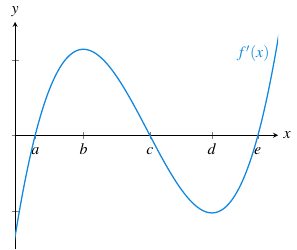
\includegraphics{././img/derivadas/grafica-ext-1.png}

\end{exercise}

\begin{tcolorbox}[enhanced jigsaw, leftrule=.75mm, rightrule=.15mm, colbacktitle=quarto-callout-tip-color!10!white, opacitybacktitle=0.6, bottomtitle=1mm, coltitle=black, colback=white, titlerule=0mm, left=2mm, arc=.35mm, breakable, colframe=quarto-callout-tip-color-frame, toprule=.15mm, toptitle=1mm, opacityback=0, title=\textcolor{quarto-callout-tip-color}{\faLightbulb}\hspace{0.5em}{Solución}, bottomrule=.15mm]

A la vista de la gráfica de \(f'(x)\) se observa que los puntos críticos
de \(f\) (los puntos que anulan la derivada) son \(x=a\) y \(x=c\) y
\(x=e\).

\textbf{Estudio del crecimiento}

Observando el signo de \(f'\) podemos estudiar el crecimiento de \(f\)
aplicando el
\href{https://aprendeconalf.es/analisis-manual/derivadas.html\#thm-crecimiento-signo-derivada}{criterio
del signo de la primera derivada}. A la vista de la gráfica se observa
que \(f'(x)>0\) \(\forall x\in (a,c)\cup (e,\infty)\), y, por tanto,
\(f\) es creciente en estos intervalos, y \(f'(x)<0\)
\(\forall x\in (-\infty, a)\cup (c,e)\), y, por tanto, \(f\) es
decreciente en estos intervalos.

\textbf{Estudio de los extremos}

Los posibles extremos de \(f\) estarán entre sus puntos críticos.
Observando el crecimiento de la \(f\) a la izquierda y a la derecha de
cada punto crítico podemos determinar si son máximos, mínimos o puntos
de inflexión.

\begin{itemize}
\tightlist
\item
  En \(x=a\) \(f\) decrece a la izquierda y crece a la derecha, luego
  hay un mínimo relativo.
\item
  En \(x=c\) \(f\) crece a la izquierda y decrece a la derecha, luego
  hay un máximo relativo.
\item
  En \(x=e\) \(f\) decrece a la izquierda y crece a la derecha, luego
  hay un mínimo relativo.
\end{itemize}

\textbf{Estudio de la concavidad}

Para estudiar la concavidad utilizaremos el
\href{https://aprendeconalf.es/analisis-manual/derivadas.html\#thm-concavidad}{criterio
del signo de la segunda derivada}. Para ver el signo de \(f''\) basta
con observar el crecimiento de \(f'\) en la gráfica ya que \(f''\) es la
derivada de \(f'\) y por tanto su signo depende del crecimiento de
\(f'\). Observando la gráfica de \(f'\) se tiene que \(f'(x)\) es
creciente en \((-\infty, b)\) y \((d,\infty)\) de manera que
\(f''(x)>0\) \(\forall x\in (-\infty, b)\cup (d,\infty)\), y, por tanto,
la \(f\) es cóncava hacia arriba en estos intervalos. Por otro lado,
\(f'(x)\) es decreciente en el intervalo \((b,d)\), por lo que
\(f''(x)<0\) \(\forall x\in(b,d)\) y, por tanto, \(f\) es cóncava hacia
abajo en este intervalo.

\textbf{Estudio de los puntos de inflexión}

Los puntos de inflexión son los puntos donde cambia la concavidad de la
función, de modo que, según el estudio de la concavidad, \(f\) tiene
puntos de inflexión en \(x=b\) y \(x=d\).

\end{tcolorbox}

\leavevmode\vadjust pre{\hypertarget{exr-extremos-2}{}}%
\begin{exercise}[]\label{exr-extremos-2}

Hallar \(a\), \(b\) y \(c\) en la función \(f(x)=x^3+bx^2+cx+d\) para
que tenga un punto de inflexión en \(x=3\), pase por el punto \((1,0)\)
y alcance un máximo en \(x=1\).

\end{exercise}

\begin{tcolorbox}[enhanced jigsaw, leftrule=.75mm, rightrule=.15mm, colbacktitle=quarto-callout-tip-color!10!white, opacitybacktitle=0.6, bottomtitle=1mm, coltitle=black, colback=white, titlerule=0mm, left=2mm, arc=.35mm, breakable, colframe=quarto-callout-tip-color-frame, toprule=.15mm, toptitle=1mm, opacityback=0, title=\textcolor{quarto-callout-tip-color}{\faLightbulb}\hspace{0.5em}{Solución}, bottomrule=.15mm]

Calculamos las dos primeras derivadas.

\begin{align*}
f'(x) &= 3x^2-2bx+c\\ 
f''(x) &= 6x-2b
\end{align*}

Para que la función tenga un punto de inflexión en \(x=3\) debe ser
\(f''(3)=0\), es decir, \(f''(3) = 6\cdot 3 - 2b = 18-2b = 0\), de donde
se deduce que \(b=9\).

Para que la función tenga un máximo en \(x=1\) debe ser \(f'(1)=0\), es
decir, \(f'(1)=3\cdot 1^2-2\cdot 9\cdot 1+c = 3-18+c = -15+c=0\), de
donde se deduce que \(c=15\).

Finalmente, para que pase por el punto \((1,0\))\$ debe ser \(f(1)=0\),
es decir, \(f(1) = 1^3-9\cdot 1^2+15\cdot 1+d = 1-9+15+d = 7+d=0\), de
donde se deduce que \(d=-7\).

\end{tcolorbox}

\leavevmode\vadjust pre{\hypertarget{exr-extremos-3}{}}%
\begin{exercise}[]\label{exr-extremos-3}

La cantidad de trigo en una cosecha \(C\) depende del nivel de nitrógeno
en el suelo \(n\) según la ecuación

\[
C(n) = \frac{n}{1+n^2},\quad n\geq 0.
\]

¿Para qué nivel de nitrógeno se obtendrá la mayor cosecha de trigo?

\end{exercise}

\begin{tcolorbox}[enhanced jigsaw, leftrule=.75mm, rightrule=.15mm, colbacktitle=quarto-callout-tip-color!10!white, opacitybacktitle=0.6, bottomtitle=1mm, coltitle=black, colback=white, titlerule=0mm, left=2mm, arc=.35mm, breakable, colframe=quarto-callout-tip-color-frame, toprule=.15mm, toptitle=1mm, opacityback=0, title=\textcolor{quarto-callout-tip-color}{\faLightbulb}\hspace{0.5em}{Solución}, bottomrule=.15mm]

Se trata de calcular el valor de \(n\) donde se alcanza el máximo de
\(C(n)\). Veremos primero si hay algún máximo relativo. Para ello
calculamos los puntos críticos.

\[
C'(n)= \frac{(n)'(1+n^2)-n(1+n^2)'}{(1+n^2)^2} = \frac{(1+n^2)-n(2n)}{(1+n^2)^2} = \frac{1-n^2}{(1+n^2)^2}
\]

\(C'(x)=0 \Leftrightarrow 1-n^2 = 0 \Leftrightarrow n^2 =1 \Leftrightarrow n=\pm 1\).

Como no tienen sentido cantidades de nitrógeno negativas, el único punto
crítico está en \(n=1\). Para ver si se trata de un máximo, estudiamos
ahora el signo de la primera derivada a la izquierda y a la derecha de
este punto. Tomando, por ejemplo \(n=0\), se tiene
\(C'(0) = \frac{1-0^2}{(1+0^2)^2} = 1>0\), por lo que la función es
creciente a la izquierda de \(n=1\). Y tomando, por ejemplo \(n=2\), se
tiene \(C'(2) = \frac{1-2^2}{(1+2^2)^2}=-3/25<0\), por lo que la función
es decreciente a la derecha de \(n=1\). Por tanto, en \(n=1\) existe un
máximo relativo, que además, es único. Como la función es continua en
todo \(\mathbb{R}\) al ser una función racional y no anularse nunca su
denominador, se tiene que el máximo absoluto coincide con el relativo,
de manera que el nivel de nitrógeno para el que la cosecha será máxima
es \(n=1\).

\end{tcolorbox}

\leavevmode\vadjust pre{\hypertarget{exr-extremos-4}{}}%
\begin{exercise}[]\label{exr-extremos-4}

La velocidad \(v\) de una reacción irreversible \(A+B\rightarrow AB\) es
función de la concentración \(x\) del producto \(AB\) y puede expresarse
según la ecuación

\[
v(x) = 4(3-x)(5-x).
\] ¿Qué valor de \(x\) maximiza la velocidad de reacción?

\end{exercise}

\begin{tcolorbox}[enhanced jigsaw, leftrule=.75mm, rightrule=.15mm, colbacktitle=quarto-callout-tip-color!10!white, opacitybacktitle=0.6, bottomtitle=1mm, coltitle=black, colback=white, titlerule=0mm, left=2mm, arc=.35mm, breakable, colframe=quarto-callout-tip-color-frame, toprule=.15mm, toptitle=1mm, opacityback=0, title=\textcolor{quarto-callout-tip-color}{\faLightbulb}\hspace{0.5em}{Solución}, bottomrule=.15mm]

Veremos primero si hay algún máximo relativo. Para ello calculamos los
puntos críticos de \$v(x)=4(3-x)(5-x)=4x\^{}2-32x+60

\[
v'(x) = 8x-32 = 0 \Leftrightarrow x = 4.
\]

Para ver si se trata de un máximo relativo, estudiamos el signo de la
segunda derivada en el punto crítico. \(v''(x)= 8>0\), luego la función
es cóncava hacia arriba en todo \(\mathbb{R}\) y en particular en
\(x=4\), por lo que tiene un mínimo local en \(x=4\).

Como el dominio de la función es \([0,\infty)\) ya que las
concentraciones no pueden ser negativas, y
\(\lim_{n\to\infty}v(x) = \lim_{x\to\infty}4x^2-32x+60=\infty\), la
función no tiene máximo local, por lo que no existe un valor de \(x\)
que maximice la velocidad de reacción.

\end{tcolorbox}

\leavevmode\vadjust pre{\hypertarget{exr-extremos-5}{}}%
\begin{exercise}[]\label{exr-extremos-5}

Un naufrago se encuentra en una isla situada en un plano con coordenadas
\((2,0)\). Se sabe que un ferry hace siempre la trayectoria dada por la
función \(f(x)=\sqrt{x+1}\). ¿Hacia qué punto de la trayectoria del
ferry debe nadar el naufrago para recorrer la menor distancia posible?
¿Qué distancia recorrerá si nada hacia ese punto?

\end{exercise}

\begin{tcolorbox}[enhanced jigsaw, leftrule=.75mm, rightrule=.15mm, colbacktitle=quarto-callout-tip-color!10!white, opacitybacktitle=0.6, bottomtitle=1mm, coltitle=black, colback=white, titlerule=0mm, left=2mm, arc=.35mm, breakable, colframe=quarto-callout-tip-color-frame, toprule=.15mm, toptitle=1mm, opacityback=0, title=\textcolor{quarto-callout-tip-color}{\faLightbulb}\hspace{0.5em}{Solución}, bottomrule=.15mm]

El ferry pasará por todos los puntos \((x,f(x))\), por lo que se trata
de averiguar el valor de \(x\) que hace mínima la distancia del punto
\((2,0)\) a \((x,f(x))\), o lo que es lo mismo, minimizar el módulo del
vector \$(x,f(x))-(2,0) = \((x-2, f(x))\), que vale

\[
|(x-2,f(x))|=\sqrt{(x-2)^2+(\sqrt{x})^2} = \sqrt{x^2-2x+4-x} = \sqrt{x^2-x+4}.
\]

Se trata, por tanto, de calcular el mínimo de la función
\(m(x)=\sqrt{x^2-x+4}\). Calculamos los puntos críticos.

\[
m'(x) = \frac{2x-1}{2\sqrt{x^2-x+4}} = 0 \Leftrightarrow 2x-1 = 0 \Leftrightarrow x=1/2.
\]

Para ver si se trata de un mínimo relativo, estudiamos el signo de la
derivada a la izquierda y a la derecha del punto crítico. Tomando, por
ejemplo, \(x=0\), se tiene
\(m'(0) = \frac{2\cdot 0-1}{2\sqrt{0^2-0+4}} = -1/4<0\), de manera que
el módulo decrece a la izquierda de \(x=1/2\). Y tomando, por ejemplo,
\(x=1\), se tiene que
\(m'(1)=\frac{2\cdot 1-1}{2\sqrt{1^2-1+4}}=1/4>0\), de manera que el
módulo crece a la derecha de \(x=1/2\). Por tanto, la función del módulo
tiene un mínimo relativo en \(x=1/2\), que además es único, y como \(m\)
es continua en todo \(\mathbb{R}\), el mínimo relativo es también mínimo
absoluto, y por tanto, el naufrago debe nadar hacia el punto
\((1/2, \sqrt{1/2})\).

\end{tcolorbox}

\leavevmode\vadjust pre{\hypertarget{exr-extremos-6}{}}%
\begin{exercise}[]\label{exr-extremos-6}

Un hotel alquila habitaciones por un precio entre 40€ y 100€ diarios. Se
ha observado que el número de habitaciones que alquilan depende del
precio \(x\) según la función \(h(x)=300-3x\). ¿Qué precio se debe
cobrar por habitación para obtener los máximos ingresos?

\end{exercise}

\begin{tcolorbox}[enhanced jigsaw, leftrule=.75mm, rightrule=.15mm, colbacktitle=quarto-callout-tip-color!10!white, opacitybacktitle=0.6, bottomtitle=1mm, coltitle=black, colback=white, titlerule=0mm, left=2mm, arc=.35mm, breakable, colframe=quarto-callout-tip-color-frame, toprule=.15mm, toptitle=1mm, opacityback=0, title=\textcolor{quarto-callout-tip-color}{\faLightbulb}\hspace{0.5em}{Solución}, bottomrule=.15mm]

Los ingresos vienen dados por la función
\(f(x) = xh(x)=x(300-3x) = 300x-3x^2\). Se trata de calcular el máximo
absoluto de esta función. Para ello veremos primero si tiene algún
máximo relativo. Calculamos los puntos críticos.

\[
f'(x) = 300-6x = 0 \Leftrightarrow x=50.
\]

Para ver si se trata de un máximo relativo, estudiamos el signo de la
segunda derivada en el punto crítico. \(f''(x)=-6<0\), por lo que la
función es cóncava hacia abajo en todo \(\mathbb{R}\), y en particular
en \(x=50\), por lo que \(f\) tiene un máximo relativo en este punto,
que además es único. Como \(f\) es continua en todo \(\mathbb{R}\), el
máximo relativo es también absoluto, y el precio de las habitaciones que
maximiza los ingresos es \(x=50\)€.

\end{tcolorbox}

\leavevmode\vadjust pre{\hypertarget{exr-extremos-7}{}}%
\begin{exercise}[]\label{exr-extremos-7}

Existen organismos que se reproducen una sola vez en su vida como por
ejemplo los salmones. En este tipo de especies, la velocidad de
incremento per cápita \(v\), que mide la capacidad reproductiva, depende
de la edad \(x\) según la ecuación

\[
v(x) = \frac{\ln(p(x)h(x))}{x},
\]

donde \(p(x)\) es la probabilidad de sobrevivir hasta la edad \(x\) y
\(h(x)\) es el número de nacimientos de hembras a la edad \(x\).
Calcular la edad óptima de reproducción, es decir, el valor que maximice
\(v\), para \(p(x)=e^{-0.1x}\) y \(h(x)=4x^{0.9}\).

\end{exercise}

\begin{tcolorbox}[enhanced jigsaw, leftrule=.75mm, rightrule=.15mm, colbacktitle=quarto-callout-tip-color!10!white, opacitybacktitle=0.6, bottomtitle=1mm, coltitle=black, colback=white, titlerule=0mm, left=2mm, arc=.35mm, breakable, colframe=quarto-callout-tip-color-frame, toprule=.15mm, toptitle=1mm, opacityback=0, title=\textcolor{quarto-callout-tip-color}{\faLightbulb}\hspace{0.5em}{Solución}, bottomrule=.15mm]

Se trata de calcular el máximo absoluto de la función

\begin{align*}
v(x) &=\frac{\ln(e^{-0.1x}4x^{0.9})}{x} = \frac{\ln(e^{-0.1x})+\ln(4)+\ln(x^{0.9})}{x}\\ 
&= \frac{-0.1x+\ln(4)+0.9\ln(x)}{x} = -0.1+\frac{\ln(4)+0.9\ln(x)}{x}.
\end{align*}

Veamos primero si la función tiene algún máximo relativo. Calculamos los
puntos críticos.

\[
\begin{gathered}
v'(x) = \frac{(x)'(\ln(4)+0.9\ln(x))-x(\ln(4)+0.9\ln(x))'}{x^2}\\ = \frac{\ln(4)+0.9\ln(x)-0.9}{x^2} = 0 \Leftrightarrow \ln(4)+0.9\ln(x)-0.9 = 0 \\ \Leftrightarrow \ln(x)=\frac{0.9-\ln(4)}{0.9} \Leftrightarrow x = e^{\frac{0.9-\ln(4)}{0.9}} \approx 0.5826.
\end{gathered}
\]

Para ver si \(v\) tiene un máximo relativo en este punto, estudiamos el
signo de la derivada a la izquierda y a la derecha del punto crítico.
Tomando, por ejemplo, \(x=0\), se tiene \(v'(0.5) \approx 0.5502 >0\),
por lo que la función crece a la izquierda de \(x=0.5826\). Y tomando,
por ejemplo, \(x=0.6\), se tiene que \(v'(0.6)\approx -0.0738<0\), por
lo que \(v\) decrece a la derecha de \(x=0.5826\), así que, \(v\) tiene
un máximo relativo en \(x=0.5826\), que además es único. Como \(v\) es
continua en \((0,\infty)\), que es el dominio que tiene sentido en el
contexto del problema, el máximo relativo es también absoluto y la edad
óptima de reproducción es a los \(0.5826\) años.

\end{tcolorbox}

\leavevmode\vadjust pre{\hypertarget{exr-extremos-8}{}}%
\begin{exercise}[]\label{exr-extremos-8}

Un lata de refresco cilíndrica contiene \(33\) cl. Hallar las
dimensiones de la lata para que la cantidad de aluminio utilizada en su
creación sea mínima.

\end{exercise}

\leavevmode\vadjust pre{\hypertarget{exr-extremos-9}{}}%
\begin{exercise}[]\label{exr-extremos-9}

La distancia en kilómetros que recorre un coche de alquiler con 1 litro
de gasolina depende de la velocidad a la que circule según la función
\(d(x)=120-x\) para \(x\in(50,120)\). Si el coste de la gasolina es de
\(2\) €/l y el coste del alquiler es de \(10\) €/h, ¿a qué velocidad
debe circular para que el coste del trayecto sea mínimo? ¿Cuál será el
coste por kilómetro si circula a esa velocidad?

\end{exercise}

\begin{tcolorbox}[enhanced jigsaw, leftrule=.75mm, rightrule=.15mm, colbacktitle=quarto-callout-tip-color!10!white, opacitybacktitle=0.6, bottomtitle=1mm, coltitle=black, colback=white, titlerule=0mm, left=2mm, arc=.35mm, breakable, colframe=quarto-callout-tip-color-frame, toprule=.15mm, toptitle=1mm, opacityback=0, title=\textcolor{quarto-callout-tip-color}{\faLightbulb}\hspace{0.5em}{Solución}, bottomrule=.15mm]

Como la distancia recorrida a una velocidad \(x\) es \(d(x)=120-x\) y,
como la velocidad es \(x=\frac{d(x)}{t}\), el tiempo necesario para
recorrer esa distancia es \(\frac{d(x)}{x}\), de manera que el coste del
alquiler para recorrer esa distancia es \(\frac{d(x)}{x}10\). A esto hay
que sumar el precio del litro de gasolina necesario para recorrer esa
distancia, de manera que el coste de recorrer esa distancia es
\(\frac{d(x)}{x}10+2\). Por tanto, el coste por kilómetro para una
velocidad \(x\) viene dado por la función

\[
c(x)=\frac{\frac{d(x)}{x}10+2}{120-x} = \frac{8x-1200}{x^2-120x}
\]

Para determinar el mínimo de la función calculamos los puntos críticos.
La derivada vale

\[
c'(x)=\frac{-8x^2+2400x-144000}{x^4-240x^3+14400 x^2}
\]

y resolviendo la ecuación \(-8x^2+2400x-144000=0\) se obtienen los
puntos críticos \(x=82.92\) y \(x=217.08\). Como el segundo punto
crítico queda fuera del rango de velocidades de 50 a 120, estudiaremos
solo el primero. Usando el criterio de la primera derivada, estudiamos
el signo de la primera derivada a la izquierda y a la derecha del punto
crítico, por ejemplo \(c'(80)=-1/3200<0\) y \(c'(83)=88/9431041>0\), por
lo que \(c\) tiene un mínimo en \(x=82.92\), es decir, la velocidad a la
que debe viajar para que el coste sea mínimo es \(82.92\) km/h, y el
precio por kilómetro a esa velocidad será \(0.17\) €/l.

\end{tcolorbox}

\leavevmode\vadjust pre{\hypertarget{exr-teorema-valor-medio}{}}%
\begin{exercise}[]\label{exr-teorema-valor-medio}

En un tramo de carretera limitado a una velocidad máxima de \(70\) km/h
existe un semáforo de tramo. Según el registro del semáforo, un vehículo
pasa por el comienzo del tramo, situado en el kilómetro 12 a las 8:00 y
pasa por el final del tramo, situado en el kilómetro \(14\), un minuto y
medio después. ¿Será sancionado el vehículo por exceso de velocidad?

\end{exercise}

\begin{tcolorbox}[enhanced jigsaw, leftrule=.75mm, rightrule=.15mm, colbacktitle=quarto-callout-tip-color!10!white, opacitybacktitle=0.6, bottomtitle=1mm, coltitle=black, colback=white, titlerule=0mm, left=2mm, arc=.35mm, breakable, colframe=quarto-callout-tip-color-frame, toprule=.15mm, toptitle=1mm, opacityback=0, title=\textcolor{quarto-callout-tip-color}{\faLightbulb}\hspace{0.5em}{Solución}, bottomrule=.15mm]

Suponiendo que la función \(f\) que determina la posición del vehículo
en cada instante es continua y derivable en el tramo del enunciado,
según el
\href{https://aprendeconalf.es/analisis-manual/derivadas.html\#thm-valor-medio}{teorema
del valor medio}, existe al menos un instante \(c\) en el que

\[
f'(c) = \frac{14-12}{8.025-8} = \frac{2}{0.025}I= 80 \mbox{ km/h}.
\]

Como \(f'\) es la velocidad instantánea, se puede concluir que en algún
momento la velocidad instantánea fue de 80 km/h, y como la máxima
velocidad permitida en el tramo es de \(70\) km/h, el vehículo será
sancionado.

\end{tcolorbox}

\leavevmode\vadjust pre{\hypertarget{exr-cinematica-1}{}}%
\begin{exercise}[]\label{exr-cinematica-1}

La posición que ocupa un coche que se mueve en línea recta, puede
expresarse en función del tiempo según la ecuación \[
e(t) = 4t^3 -2t +1.
\] Calcular su velocidad y aceleración en cualquier instante.\\
Nota: La aceleración es la tasa de variación instantánea de la
velocidad.

\end{exercise}

\begin{tcolorbox}[enhanced jigsaw, leftrule=.75mm, rightrule=.15mm, colbacktitle=quarto-callout-tip-color!10!white, opacitybacktitle=0.6, bottomtitle=1mm, coltitle=black, colback=white, titlerule=0mm, left=2mm, arc=.35mm, breakable, colframe=quarto-callout-tip-color-frame, toprule=.15mm, toptitle=1mm, opacityback=0, title=\textcolor{quarto-callout-tip-color}{\faLightbulb}\hspace{0.5em}{Solución}, bottomrule=.15mm]

La velocidad es la tasa de variación instantánea del espacio con
respecto al tiempo, es decir, la primera derivada de \(e\), que vale
\(e'(t)=12t^2-2\).

La aceleración es la tasa de variación instantánea de la velocidad con
respecto al tiempo, es decir, la segunda derivada de \(e\), que vale
\(e''(t) = 24t\).

\end{tcolorbox}

\leavevmode\vadjust pre{\hypertarget{exr-cinematica-2}{}}%
\begin{exercise}[]\label{exr-cinematica-2}

El espacio recorrido por un objeto que se lanza verticalmente hacia
arriba, sin tener en cuenta la resistencia del aire, viene dado por la
ecuación \[
e(t) =v_0t-\frac{1}{2}gt^2
\] donde \(v_0\) es la velocidad inicial con que se lanza el objeto,
\(g=9.81\) m/s\(^2\) es la aceleración de la gravedad en la superfice
terrrestre y \(t\) es el tiempo transcurrido desde que el objeto se
lanza.

\begin{enumerate}
\def\labelenumi{\alph{enumi}.}
\tightlist
\item
  Calcular la velocidad y la aceleración en cualquier instante.
\item
  Si el objeto se lanza inicialmente a 50 km/h, ¿cuál será la altura
  máxima que alcanzará el objeto? ¿Cuál será su velocidad en ese
  momento?
\item
  ¿En qué instante volverá a tocar la tierra el objeto? ¿Con qué
  velocidad?
\end{enumerate}

\end{exercise}

\begin{tcolorbox}[enhanced jigsaw, leftrule=.75mm, rightrule=.15mm, colbacktitle=quarto-callout-tip-color!10!white, opacitybacktitle=0.6, bottomtitle=1mm, coltitle=black, colback=white, titlerule=0mm, left=2mm, arc=.35mm, breakable, colframe=quarto-callout-tip-color-frame, toprule=.15mm, toptitle=1mm, opacityback=0, title=\textcolor{quarto-callout-tip-color}{\faLightbulb}\hspace{0.5em}{Solución}, bottomrule=.15mm]

\begin{enumerate}
\def\labelenumi{\alph{enumi}.}
\item
  La velocidad es la tasa se variación instantánea con respecto al
  tiempo, es decir, la primera derivada de \(e\), que vale,
  \(e'(t) = v_0-gt\). Y la aceleración es la tasa de variación
  instantánea de la velocidad con respecto al tiempo, es decir, la
  segunda derivada de \(e\), que vale \(e''(t)=-g\).
\item
  Para ver en qué punto el objeto alcanza la altura máxima, estudiamos
  primero si la función tiene un máximo relativo. Calculamos los puntos
  críticos, tomando \(v_0 = 50\) km/h = \(\frac{125}{9}\) m/s.

  \[
   e'(t) = \frac{125}{9}-9.81t = 0 \Leftrightarrow t \approx 1.42 \mbox{s}.
   \]

  Para ver si se trata de un máximo relativo, estudiamos el signo de la
  segunda derivada en el punto. Como \(e''(t)=-9.81<0\) la función es
  cóncava hacia abajo en todo \(\mathbb{R}\), y en particular en
  \(t\approx 1.42\), de manera que \(e\) tiene un máximo relativo en
  \(t\approx 1.42\), que además es único. Como la función es continua en
  todo \(\mathbb{R}\), el máximo relativo es también absoluto, y por
  tanto, la altura máxima que alcanzará el objeto es aproximadamente
  \$e(1.42)=\(9.83\) m. En ese instante, la velocidad del objeto será
  nula ya que se trata de un punto crítico y \(e'(1.42)=0\).
\item
  Para ver cuándo el objeto vuelve a tocar el suelo basta con resolver
  la ecuación

  \[
   e(t)=50t-\frac{1}{2}9.81t^2 =0 \Leftrightarrow t(50-4.905t) = 0 \Leftrightarrow t=0 \mbox{ o } t\approx 2.83 \mbox{ s}.
   \]

  Por tanto, el objeto volverá a tocar suelo a los \(2.83\) segundos
  aproximadamente. En ese instante la velocidad será
  \(e'(2.83)=\frac{125}{9}-9.81\cdot 2.83 \approx -13.89\) m/s, que es
  la misma velocidad con la que se lanzó pero negativa.
\end{enumerate}

\end{tcolorbox}

\leavevmode\vadjust pre{\hypertarget{exr-trayectorias-1}{}}%
\begin{exercise}[]\label{exr-trayectorias-1}

Una partícula se mueve a lo largo de la curva

\[
\begin{cases}
x = \operatorname{tg}(t),  \\
y = t^2-2t+3. \\
\end{cases}
\]

donde \(x\) e \(y\) están medidos en metros y el tiempo \(t\) en
segundos.

\begin{enumerate}
\def\labelenumi{\alph{enumi}.}
\tightlist
\item
  Hallar \(\frac{dy}{dx}\) en \(t=0\).
\item
  Hallar la tangente a la trayectoria en el punto \((0,3)\).
\end{enumerate}

\end{exercise}

\begin{tcolorbox}[enhanced jigsaw, leftrule=.75mm, rightrule=.15mm, colbacktitle=quarto-callout-tip-color!10!white, opacitybacktitle=0.6, bottomtitle=1mm, coltitle=black, colback=white, titlerule=0mm, left=2mm, arc=.35mm, breakable, colframe=quarto-callout-tip-color-frame, toprule=.15mm, toptitle=1mm, opacityback=0, title=\textcolor{quarto-callout-tip-color}{\faLightbulb}\hspace{0.5em}{Solución}, bottomrule=.15mm]

\begin{enumerate}
\def\labelenumi{\alph{enumi}.}
\item
  Aplicando la regla de la cadena se tiene que

  \[
   \dfrac{dy}{dt} = \dfrac{dy}{dx}\dfrac{dx}{dt},
   \]

  y en consecuencia,

  \[
   \dfrac{dy}{dx}(t) = \frac{dy/dt}{dx/dt}(t)=\frac{2t-2}{1+\operatorname{tg}(t)^2}.
   \]

  En el punto \(t=0\) tendremos

  \[
   \dfrac{dy}{dx}(0) = \frac{-2}{1+\operatorname{tg}(0)^2} = -2.
   \]
\item
  La ecuación de la recta tangente a la trayectoria en el punto
  \((x(t_0),y(t_0))\) correspondiente al instante \(t_0,\) viene dada
  por la expresión

  \[
   y-y(t_0) = \dfrac{dy}{dx}(t_0)(x-x(t_0)).
   \]

  Como el punto \((0,3)\) se alcanza precisamente en el instante \(t=0\)
  tenemos que la ecuación de la recta tangente a la trayectoria en dicho
  instante es:

  \[
   y-y(0) = \dfrac{dy}{dx}(0)(x-x(0)),
   \]

  es decir,

  \[
   y-3 = -2(x-0),
   \]

  y simplificando obtenemos:

  \[
   y = 3-2x.
   \]
\end{enumerate}

\end{tcolorbox}

\leavevmode\vadjust pre{\hypertarget{exr-trayectorias-2}{}}%
\begin{exercise}[]\label{exr-trayectorias-2}

Las coordenadas paramétricas de un punto material lanzado bajo un ángulo
respecto al horizonte son

\[
\begin{cases}
x=v_0t, & \\
y=-\frac{1}{2}gt^2
\end{cases}
\]

donde \(t\in \mathbb{R}^{+}\) es el tiempo contado a partir del instante
en que el punto llega a la posición más alta, \(v_0\) es la velocidad
horizontal en el instante \(t=0\) y \(g=9.81\) m\(^2\)/s es la
aceleración de la gravedad en la superficie terrestre. ¿En qué instante
la magnitud de la velocidad horizontal será igual a la de la velocidad
vertical? ¿Cuánto debería valer \(v_0\) para que en dicho instante el
punto haya recorrido 100 m horizontalmente? Calcular la ecuación de la
recta tangente en dicho instante con el valor de \(v_0\) calculado.

\end{exercise}

\begin{tcolorbox}[enhanced jigsaw, leftrule=.75mm, rightrule=.15mm, colbacktitle=quarto-callout-tip-color!10!white, opacitybacktitle=0.6, bottomtitle=1mm, coltitle=black, colback=white, titlerule=0mm, left=2mm, arc=.35mm, breakable, colframe=quarto-callout-tip-color-frame, toprule=.15mm, toptitle=1mm, opacityback=0, title=\textcolor{quarto-callout-tip-color}{\faLightbulb}\hspace{0.5em}{Solución}, bottomrule=.15mm]

La velocidad horizontal es la derivada del espacio recorrido
horizontalmente (componente \(x\)) con respecto al tiempo, es decir,

\[
\frac{dx}{dt} = \frac{d}{dt}(v_0t)=v_0.
\]

Del mismo modo, la velocidad vertical es la derivada del espacio
recorrido verticalmente (componente \(y\)) en relación al tiempo,

\[
\frac{dy}{dt} = \frac{d}{dt}(-\frac{1}{2}gt^2)=-gt
\]

Para ver en qué instante ambas magnitudes serán iguales, las igualamos y
resolvemos la ecuación:

\[
|\frac{dx}{dt}|=|\frac{dy}{dt}| \Leftrightarrow v_0 = gt \Leftrightarrow t=\frac{v_0}{g}=\frac{v_0}{9.81} s.
\]

Para que en dicho instante el punto haya recorrido 100 m
horizontalmente, debe cumplirse que \(x(v_0/9.81)=100\) m, de lo que se
deduce:

\[
x(v_0/9.81)=v_0\frac{v_0}{9.81} = \frac{v_0^2}{9.81}=100 \Leftrightarrow v_0^2 = 981 \Leftrightarrow v_0 = +\sqrt{981}= 31.32 \mbox{ m/s}.
\]

Por tanto, el instance en cuestión es \(t=v_0/9.81= 31.32/9.81 = 3.19\)
s.

Por último, la ecuación de la recta tangente en dicho instante, para el
valor de \(v_0\) calculado es:

\[
y = y(3.19) + \frac{dy}{dx}(3.19) (x-x(3.19))
\]

Ya hemos visto que \(x(3.19)=100\), y que en dicho instante la velocidad
horizontal y vertical coinciden, de manera que

\[
\frac{dy}{dx}(3.19)=\frac{dy/dt}{dx/dt}=-1,
\]

de modo que sólo nos queda calcular el espacio vertical recorrido en
dicho instante, que es

\[
y(3.19)=-\frac{1}{2}9.81\cdot 3.19^2= -49.91.
\]

Sustituyendo en la ecuación anterior llegamos a la recta tangente: \[
y = -49.91-(x-100) \Leftrightarrow y=-x+50.09.
\]

\end{tcolorbox}

\leavevmode\vadjust pre{\hypertarget{exr-derivadas-parametricas-1}{}}%
\begin{exercise}[]\label{exr-derivadas-parametricas-1}

La cantidad de árboles en un ecosistema depende del tiempo según la
función \(a(t)=100\ln(t^2+1)\), y la cantidad de un determinado parásito
de los árboles, también depende del tiempo según la función
\(p(t) = \sqrt[3]{t^2+ 2}\). Calcular la tasa de variación instantánea
del número de parásitos en relación al número de árboles, en el instante
en que el número de parásitos es \(3\).

\end{exercise}

\begin{tcolorbox}[enhanced jigsaw, leftrule=.75mm, rightrule=.15mm, colbacktitle=quarto-callout-tip-color!10!white, opacitybacktitle=0.6, bottomtitle=1mm, coltitle=black, colback=white, titlerule=0mm, left=2mm, arc=.35mm, breakable, colframe=quarto-callout-tip-color-frame, toprule=.15mm, toptitle=1mm, opacityback=0, title=\textcolor{quarto-callout-tip-color}{\faLightbulb}\hspace{0.5em}{Solución}, bottomrule=.15mm]

\[
\frac{da}{dp} = \frac{da/dt}{dp/dt} = \frac{\frac{200t}{t^2+1}}{\frac{2t}{3\sqrt[3]{(t^2+2)^2}}} = \frac{200t\cdot 3\sqrt[3]{(t^2+2)^2}}{2t(t^2+1)} = \frac{600t\sqrt[3]{(t^2+2)^2}}{2t^3+2t}.
\]

El instante en el que el número de parásitos es \(3\) es

\[
p(t)=\sqrt[3]{t^2+2} = 3 \Leftrightarrow t^2+2 = 27 \Leftrightarrow t^2=25 \Leftrightarrow t=\pm 5.
\]

Como en el contexto del problema podemos suponer que el tiempo es
positivo, el instante en el que el número de parásitos es \(3\) es
\(t=5\), y

\[
\frac{da}{dp} (t=3) = \frac{600\cdot 5\sqrt[3]{(5^2+2)^2}}{2\cdot 5^3+2\cdot 5} \approx 103.85 \mbox{ árboles/parásitos}.
\]

\end{tcolorbox}

\leavevmode\vadjust pre{\hypertarget{exr-derivada-implicita-1}{}}%
\begin{exercise}[]\label{exr-derivada-implicita-1}

Dada la función \(xy+e^x-\log y=0\), calcular las ecuaciones de las
rectas tangente y normal a ella en \(x=0\).

\end{exercise}

\begin{tcolorbox}[enhanced jigsaw, leftrule=.75mm, rightrule=.15mm, colbacktitle=quarto-callout-tip-color!10!white, opacitybacktitle=0.6, bottomtitle=1mm, coltitle=black, colback=white, titlerule=0mm, left=2mm, arc=.35mm, breakable, colframe=quarto-callout-tip-color-frame, toprule=.15mm, toptitle=1mm, opacityback=0, title=\textcolor{quarto-callout-tip-color}{\faLightbulb}\hspace{0.5em}{Solución}, bottomrule=.15mm]

Sustituyendo \(x=0\) en la ecuación de la curva implícita se tiene

\[
0\cdot y + e^0-\ln(y) = 0 \Leftrightarrow \ln(y) = 1 \Leftrightarrow y=e.
\]

Así pues, hay que calcular la ecuación de las rectas tangente y normal
en el punto \((0,e)\).

La ecuación de la recta tangente en \((0,e)\) es
\(y=e+\frac{dy}{dx}(x=0)(x-0)\). Para calcular \(\frac{dy}{dx}\) tenemos
que derivar implícitamente la ecuación de la curva.

\[
\begin{gathered}
(xy+e^x-\ln(y))'=(0)' \Leftrightarrow y+xy'+e^x-\frac{y'}{y} = 0 \\ 
\Leftrightarrow xy'-\frac{y'}{y} = -y-e^x \Leftrightarrow y'(x-\frac{1}{y}) = -y-e^x \\ 
\Leftrightarrow y'\frac{xy-1}{y}=-y-e^x \Leftrightarrow y' = \frac{(-y-e^x)y}{xy-1},
\end{gathered}
\]

que en el punto \((0,e)\) vale

\[
\frac{dy}{dx}(0,e) = \frac{(-e-e^0)e}{0e-1} = e^2+e.
\]

Así pues, la ecuación de la recta tangente a la curva implícita en el
punto \((0,e)\) es \(y = e+(e^2+e)x\).

Por otro lado, la ecuación de la recta normal a la curva implícita en el
punto \((0,e)\) es
\(y=e-\frac{1}{dy/dx (x=0)}(x-0) = e-\frac{x}{e^2+e}\).

\end{tcolorbox}

\leavevmode\vadjust pre{\hypertarget{exr-derivada-implicita-2}{}}%
\begin{exercise}[]\label{exr-derivada-implicita-2}

Suponiendo que la temperatura, \(T\) en grados centígrados, y el
volumen, \(V\) en metros cúbicos, de un gas real encerrado en un
contenedor de volumen variable están relacionados mediante la siguiente
ecuación:

\[
T^2(V^2-\pi^2)-V\cos(TV) = 0.
\]

\begin{enumerate}
\def\labelenumi{\alph{enumi}.}
\item
  Calcular la derivada del volumen con respecto a la temperatura en el
  momento en el que el volumen es de \(\pi\) m\(^3\) y la temperatura es
  medio grado centígrado.
\item
  ¿Cuál sería la ecuación de la recta tangente a la gráfica de la
  función que daría el volumen en función de la temperatura en el mismo
  punto del apartado anterior? Suponiendo que tanto la temperatura como
  el volumen son, a su vez, funciones de la presión, qué ecuación
  ligaría la derivada de la temperatura con respecto a la presión con la
  derivada del volumen con respecto a la presión.
\end{enumerate}

\end{exercise}

\begin{tcolorbox}[enhanced jigsaw, leftrule=.75mm, rightrule=.15mm, colbacktitle=quarto-callout-tip-color!10!white, opacitybacktitle=0.6, bottomtitle=1mm, coltitle=black, colback=white, titlerule=0mm, left=2mm, arc=.35mm, breakable, colframe=quarto-callout-tip-color-frame, toprule=.15mm, toptitle=1mm, opacityback=0, title=\textcolor{quarto-callout-tip-color}{\faLightbulb}\hspace{0.5em}{Solución}, bottomrule=.15mm]

\begin{enumerate}
\def\labelenumi{\alph{enumi}.}
\item
  \(\frac{dV}{dT} = \frac{-2T(V^2-\pi^2)-V^2\operatorname{sen}(TV)}{2T^2V-\cos(TV)+TV\operatorname{sen}(TV)}\)
  y \(\frac{dV}{dT}(V=\pi,T=0.5)= -\pi\) m\(^3\)/ºC.
\item
  Tangente: \(V=\pi(-T+1.5)\).
\item
  \(2T\frac{dT}{dP}(V^2-\pi^2)+T^2(2V\frac{dV}{dT})-\frac{dV}{dT}\cos(VT)-V(-\operatorname{sen}(TV)(\frac{dT}{dP}V+T\frac{dV}{dP})) =0\).
\end{enumerate}

\end{tcolorbox}

\leavevmode\vadjust pre{\hypertarget{exr-derivada-implicita-3}{}}%
\begin{exercise}[]\label{exr-derivada-implicita-3}

Un cuerpo se mueve en el plano a través de los puntos de coordenadas
\((x,y)\) relacionadas mediante la siguiente expresión: \[
2e^{xy} \operatorname{sen}(x) + y\cos(x) = 2.
\]

\begin{enumerate}
\def\labelenumi{\alph{enumi}.}
\tightlist
\item
  Calcular su posición cuando \(x=\pi/2\).
\item
  Calcular la ecuación de la recta tangente a la gráfica de la función
  cuando \(x=0\).
\end{enumerate}

\end{exercise}

\begin{tcolorbox}[enhanced jigsaw, leftrule=.75mm, rightrule=.15mm, colbacktitle=quarto-callout-tip-color!10!white, opacitybacktitle=0.6, bottomtitle=1mm, coltitle=black, colback=white, titlerule=0mm, left=2mm, arc=.35mm, breakable, colframe=quarto-callout-tip-color-frame, toprule=.15mm, toptitle=1mm, opacityback=0, title=\textcolor{quarto-callout-tip-color}{\faLightbulb}\hspace{0.5em}{Solución}, bottomrule=.15mm]

\begin{enumerate}
\def\labelenumi{\alph{enumi}.}
\item
  El punto \((x,y)\) en el que se encontrará el cuerpo cuando \(x=0\)
  cumple la ecuación del enunciado, de manera que sustituyendo \(x=0\),
  se tiene

  \[
   2e^0 \operatorname{sen}(0) + y \cos(0) = 2 \Leftrightarrow y = 2.
   \]

  Por tanto el cuerpo se encontrará en la posición \((0,2)\).
\item
  Sabemos que la ecuación de la recta tangente a la gráfica de la
  función en el punto de coordenadas \((x_0,y_0)\) es:

  \[
   y-y_0=\frac{dy}{dx}(x_0)(x-x_0)
   \]

  En nuestro caso, no tenemos la expresión explícita de la función
  \(y=f(x)\), pero sí que tenemos la expresión de partida que define a
  \(y\) como función de \(x\) de forma implícita. Suponiendo que \(y\)
  es función de \(x\) y derivando implícitamente con respecto a \(x\),
  obtenemos:

  \[
   2 e^{xy}(y + xy')\operatorname{sen}(x) + 2e^{xy}\cos(x) + y'\cos(x) - y\operatorname{sen}(x) = 0
   \]

  Y sacando como factor común \(y'\) y despejando, nos queda:

  \[
   y' = \frac{{ - 2e^{xy} y \operatorname{sen}(x) - 2e^{xy} \cos(x) + y \operatorname{sen}(x)}}{{2xe^{xy} \operatorname{sen}(x) + \cos(x)}}
   \]

  Y en el punto \((0,2)\) vale

  \[
   y'(0,2) = \frac{{-2e^0 \cos(0)}}{{\cos(0)}} = -2.
   \]

  Por lo tanto, la ecuación de la recta tangente es:

  \[
   y-2=-2(x-0)\Leftrightarrow y=-2x+2.
   \]
\end{enumerate}

\end{tcolorbox}

\leavevmode\vadjust pre{\hypertarget{exr-derivada-implicita-4}{}}%
\begin{exercise}[]\label{exr-derivada-implicita-4}

Hallar la ecuación de la recta tangente y normal a la curva
\(x^2+y^2=3xy-1\) en los puntos en que \(x=1\). Calcular también los
extremos relativos y decir si son máximos o mínimos.

\end{exercise}

\begin{tcolorbox}[enhanced jigsaw, leftrule=.75mm, rightrule=.15mm, colbacktitle=quarto-callout-tip-color!10!white, opacitybacktitle=0.6, bottomtitle=1mm, coltitle=black, colback=white, titlerule=0mm, left=2mm, arc=.35mm, breakable, colframe=quarto-callout-tip-color-frame, toprule=.15mm, toptitle=1mm, opacityback=0, title=\textcolor{quarto-callout-tip-color}{\faLightbulb}\hspace{0.5em}{Solución}, bottomrule=.15mm]

Consideremos \(y\) como función de \(x\). Veamos primero los puntos de
la curva en los que \(x=1\):

\[
1^{2}+y^{2} = 3\cdot 1\cdot y-1 \Leftrightarrow y^{2} -3y+2 = 0.
\]

Resolviendo la ecuación obtenemos dos soluciones \(y=1\) e \(y=2\), de
modo que existen dos puntos para los que \(x=1\), que son el \((1,1)\) y
el \((1,2)\).

Para calcular las ecuaciones de las rectas tangente y normal en estos
puntos, necesitamos calcular la derivada \(dy/dx\) en dichos puntos.
Derivamos implícitamente:

\[
\begin{gathered}
d(x^{2}+y^{2} = d(3xy-1) \Leftrightarrow 2xdx+2ydy = 3(dxy+xdy) \\ \Leftrightarrow (2x-3y)dx+(2y-3x)dy = 0,
\end{gathered}
\]

de donde se deduce

\[
\frac{dy}{dx} = \frac{3y-2x}{2y-3x},
\]

que en el punto \((1,1)\) vale

\[
\frac{dy}{dx} = \frac{3\cdot 1 - 2\cdot 1}{2\cdot 1-3\cdot 1} = -1,
\]

y en el punto \((1,2)\) vale

\[
\frac{dy}{dx} = \frac{3\cdot 2 - 2\cdot 1}{2\cdot 2-3\cdot 1} = 4.
\]

Así pues, la ecuación de la recta tangente en el punto \((1,1)\) es

\[
y-1 = \frac{dy}{dx}(1,1)(x-1) \Leftrightarrow y= 2-x,
\]

y la ecuación de la recta normal es

\[
y-1 = -\frac{1}{dy/dx}(1,1)(x-1) \Leftrightarrow y= x,
\]

mientras que la ecuación de la recta tangente en el punto \((1,2)\) es

\[
y-2 = \frac{dy}{dx}(1,2)(x-1) \Leftrightarrow y= 4x-2,
\]

y la ecuación de la recta normal es

\[
y-2 = -\frac{1}{dy/dx}(1,2)(x-1) \Leftrightarrow y=\frac{9-x}{4}.
\]

Por otro lado, para calcular los extremos relativos, primero calculamos
los puntos críticos, que son los que anulan la primera derivada:

\[
\frac{dy}{dx}=\frac{3y-2x}{2y-3x}=0 \Leftrightarrow 3y-2x=0 \Leftrightarrow y=2x/3.
\]

Pero además deben cumplir la ecuación de la curva implícita,

\[
\begin{gathered}
x^{2}+(2x/3)^{2}=3x(2x/3)-1 \Leftrightarrow x^{2}+4x^{2}/9 = 2x^{2}-1\\  \Leftrightarrow x^{2}=9/5 \Leftrightarrow x=\pm 3/\sqrt{5}.
\end{gathered}
\]

Así pues, existen dos puntos críticos que son el
\((3/\sqrt{5},2/\sqrt{5})\) y \((-3/\sqrt{5},-2/\sqrt{5})\). Para ver si
son puntos de máximo o mínimo relativos, necesitamos calcular la segunda
derivada en dichos puntos:

\[
\frac{d^{2}y}{dx^{2}}= \frac{d}{dx}\left(\frac{3y-2x}{2y-3x}\right) = \frac{(3\frac{dy}{dx}-2)(2y-3x)-(2\frac{dy}{dx}-3)(3y-2x)}{(2y-3x)^{2}}.
\]

En el punto, \((3/\sqrt{5},2/\sqrt{5})\) la segunda derivada vale

\[
\frac{d^{2}y}{dx^{2}}(3/\sqrt{5},2/\sqrt{5})=
\frac{(3\cdot 0-2)(2\frac{2}{\sqrt{5}}-3\frac{3}{\sqrt{5}})-(2\cdot 0-3)(3\frac{2}{\sqrt{5}}-2\frac{3}{\sqrt{5}})}{(2\frac{2}{\sqrt{5}}-3\frac{3}{\sqrt{5}})^{2}} = 2\sqrt{5},
\]

que al ser positiva, indica que el punto \((3/\sqrt{5},2/\sqrt{5})\) es
un punto de mínimo relativo.

En el punto, \((-3/\sqrt{5},-2/\sqrt{5})\) la segunda derivada vale

\[
\frac{d^{2}y}{dx^{2}}(-3/\sqrt{5},-2/\sqrt{5})=
\frac{(3\cdot 0-2)(2\frac{-2}{\sqrt{5}}-3\frac{-3}{\sqrt{5}})-(2\cdot 0-3)(3\frac{-2}{\sqrt{5}}-2\frac{-3}{\sqrt{5}})}{(2\frac{-2}{\sqrt{5}}-3\frac{--3}{\sqrt{5}})^{2}} = -2\sqrt{5},
\]

que al ser negativa, indica que el punto \((-3/\sqrt{5},-2/\sqrt{5})\)
es un punto de máximo relativo.

\end{tcolorbox}

\leavevmode\vadjust pre{\hypertarget{exr-derivada-implicita-5}{}}%
\begin{exercise}[]\label{exr-derivada-implicita-5}

Dada la curva \(x^2-xy+y^2=3\),

\begin{enumerate}
\def\labelenumi{\alph{enumi}.}
\tightlist
\item
  Calcular los posibles extremos relativos de \(y\), considerando \(y\)
  como función implícita de \(x\). ¿En qué puntos se alcanzan dichos
  valores?
\item
  Analizar si lo puntos anteriores son máximos o mínimos haciendo uso de
  la derivada segunda.
\end{enumerate}

\end{exercise}

\begin{tcolorbox}[enhanced jigsaw, leftrule=.75mm, rightrule=.15mm, colbacktitle=quarto-callout-tip-color!10!white, opacitybacktitle=0.6, bottomtitle=1mm, coltitle=black, colback=white, titlerule=0mm, left=2mm, arc=.35mm, breakable, colframe=quarto-callout-tip-color-frame, toprule=.15mm, toptitle=1mm, opacityback=0, title=\textcolor{quarto-callout-tip-color}{\faLightbulb}\hspace{0.5em}{Solución}, bottomrule=.15mm]

\begin{enumerate}
\def\labelenumi{\alph{enumi}.}
\item
  Derivamos implícitamente la ecuación

  \[
   \frac{d}{dx}(x^2-xy+y^2)=\frac{d}{dx}3=0
   \]

  Derivando el lado izquierdo tenemos \begin{align*}
   \frac{d}{dx}(x^2-xy+y^2) &=
   \frac{d}{dx}(x^2)-\frac{d}{dx}(xy)+\frac{d}{dx}(y^2)=\\ 
   &= 2x-(\frac{dx}{dx}y+x\frac{dy}{dx})+2y\frac{dy}{dx}=\\
   &= 2x-y-x\frac{dy}{dx}+2y\frac{dy}{dx}\\ 
   &= 2x-y+(2y-x)\frac{dy}{dx}=0
   \end{align*}

  Los posibles extremos serán los puntos donde se anule la derivada, es
  decir, \(\dfrac{dy}{dx}=0\). Sustituyendo en la ecuación anterior
  tenemos

  \[
   2x-y+(2y-x)\cdot 0= 2x-y=0 \Leftrightarrow y=2x.
   \]

  Y sustituyendo ahora en la ecuación de la función tenemos

  \[
   x^2-x\cdot 2x+(2x)^2=3 \Leftrightarrow x^2-2x^2+4x^2=3 \Leftrightarrow 3x^2=3 \Leftrightarrow x=\pm1.
   \]

  Por tanto, los posibles puntos de extremo serán (1,2) y (-1,-2).
\item
  Para ver si los puntos anteriores son efectivamente extremos,
  calculamos la derivada segunda en dichos puntos.

  \begin{align*}
   \frac{d^2}{dx^2}(x^2-xy+y^2)&=
   \frac{d}{dx}\left(\frac{d}{dx}(x^2-xy+y^2)\right)=\\
   &=\frac{d}{dx}\left(2x-y+(2y-x)\frac{dy}{dx}\right)=\\
   &=\frac{d}{dx}(2x)-\frac{d}{dx}y+\left(\frac{d}{dx}(2y-x)\frac{dy}{dx}+(2y-x)\frac{d}{dx}\frac{dy}{dx}\right)=\\
   &=2-\frac{dy}{dx}+\left(2\frac{dy}{dx}-\frac{dx}{dx}\right)\frac{dy}{dx}+(2y-x)\frac{d^2y}{dx^2}=\\
   &= 2-\frac{dy}{dx}+2\frac{d^2y}{dx^2}-\frac{dy}{dx}+(2y-x)\frac{d^2y}{dx^2}\\ 
   &= 2-2\frac{dy}{dx}+(2y-x+2)\frac{d^2y}{dx^2}=0
   \end{align*}

  Para el primer punto tenemos que sustituir \(x=1\), \(y=2\) y
  \(\dfrac{dy}{dx}=0\), y queda

  \[
   2-2\cdot 0+(2\cdot 2-1+2)\frac{d^2y}{dx^2}=0 \Leftrightarrow 2+5\frac{d^2y}{dx^2}=0 \Leftrightarrow \frac{d^2y}{dx^2}=\frac{-2}{5},
   \]

  que al ser negativo indica que el en el punto \((1,2)\) hay un máximo
  relativo.

  Para el segundo punto tenemos que sustituir \(x=-1\), \(y=-2\) y
  \(\dfrac{dy}{dx}=0\), y queda

  \[
   2-2\cdot 0+(2\cdot (-2)-(-1)1+2)\frac{d^2y}{dx^2}=0 \Leftrightarrow 2-\frac{d^2y}{dx^2}=0 \Leftrightarrow \frac{d^2y}{dx^2}=2,
   \]

  que al ser positivo indica que el en el punto \((-1,-2)\) hay un
  mínimo relativo.
\end{enumerate}

\end{tcolorbox}

\leavevmode\vadjust pre{\hypertarget{exr-taylor-1}{}}%
\begin{exercise}[]\label{exr-taylor-1}

Dada la función \(f(x)=\operatorname{sen}(x)\), se pide:

\begin{enumerate}
\def\labelenumi{\alph{enumi}.}
\tightlist
\item
  Obtener el polinomio de Taylor de tercer grado de \(f\) en el punto
  \(a=\pi/6\) y usarlo para aproximar \(\operatorname{sen}(1/2)\) dando
  una cota del error cometido.
\item
  Dar una aproximación de \(\operatorname{sen}(1/2)\) usando un el
  polinomio de Taylor de quinto grado en el punto \(a=0\), acotando el
  error cometido.
\end{enumerate}

\end{exercise}

\begin{tcolorbox}[enhanced jigsaw, leftrule=.75mm, rightrule=.15mm, colbacktitle=quarto-callout-tip-color!10!white, opacitybacktitle=0.6, bottomtitle=1mm, coltitle=black, colback=white, titlerule=0mm, left=2mm, arc=.35mm, breakable, colframe=quarto-callout-tip-color-frame, toprule=.15mm, toptitle=1mm, opacityback=0, title=\textcolor{quarto-callout-tip-color}{\faLightbulb}\hspace{0.5em}{Solución}, bottomrule=.15mm]

\begin{enumerate}
\def\labelenumi{\alph{enumi}.}
\item
  La fórmula del polinomio de Taylor de tercer grado de \(f\) en el
  punto \(a=\pi/6\) es

  \[
   P^3_{f,\pi/6}(x) = f(\pi/6)+f'(\pi/6)(x-\pi/6)+ \frac{f''(\pi/6)}{2}(x-\pi/6)^2+\frac{f'''(\pi/6)}{3!}(x-\pi/6)^3.
   \]

  Necesitamos calcular, por tanto, hasta la tercera derivada en el punto
  \(a=\pi/6\).

  \[
   \begin{array}{lll}
   f(x) = \operatorname{sen}(x) &\quad &  f(\pi/6) = 0.5\\ 
   f'(x)=\cos(x) &\quad & f'(\pi/6) = \sqrt{3}/2\\ 
   f''(x) = -\operatorname{sen}(x) &\quad & f''(\pi/6) = -0.5\\ 
   f'''(x) = -\cos(x) &\quad & f'''(\pi/6) = -\sqrt{3}/2.
   \end{array}
   \]

  Así pues, sustituyendo en la ecuación del polinomio anterior se llega
  a

  \[
   P^3_{f,\pi/6}(x) = \frac{1}{2}+\frac{\sqrt{3}}{2}(x-\pi/6)-\frac{1}{4}(x-\pi/6)^2-\frac{\sqrt{3}}{12}(x-\pi/6)^3.
   \]

  Sustituyendo en \(x=1/2\) se tiene que
  \(\operatorname{sen}(1/2) \approx P^3_{f,\pi/6}(1/2) = 0.4794255322\).

  El error cometido en la aproximación es el resto
  \(R^3_{f,\pi/6}(1/2)\). Expresando el resto de Taylor en la forma de
  Lagrange se tiene

  \[
   R^3_{f,\pi/6}(1/2) = \frac{f''''(x)}{4!}\left(\frac{1}{2}-\frac{\pi}{6}\right)^4 = \frac{\operatorname{sen}(x)}{24}\left(\frac{1}{2}-\frac{\pi}{6}\right)^4 \mbox{ con }x\in\left(\frac{1}{2}-\frac{\pi}{6}\right).
   \]

  Como \(|\operatorname{sen}(x)|\leq 1\) \(\forall x\in \mathbb{R}\), se
  tiene que una cota del error cometido es

  \[
   |R^3_{f,\pi/6}(1/2)|\leq \frac{1}{24}\left(\frac{1}{2}-\frac{\pi}{6}\right)^4 = 6.46\cdot 10^{-9}.
   \]
\item
  La fórmula del polinomio de MacLaurin de quinto grado de \(f\) es

  \[
   P^3_{f,0}(x) = f(0)+f'(0)x+ \frac{f''(0)}{2}x^2+\frac{f'''(0)}{3!}x^3+ \frac{f''''(0)}{4!}x^4+\frac{f'''''(0)}{5!}x^5
   \]
\end{enumerate}

Calculando hasta la quinta derivada en \(0\) y sustituyendo en esta
fórmula se tiene \[
P^5_{f,0}(x) = x -\frac{1}{6} x^3 + \frac{1}{120}x^5.
\]

Sustituyendo en \(x=1/2\) se tiene que
\(\operatorname{sen}(1/2) \approx P^5_{f,0}(1/2) = 0.4794270833\), y
podemos obtener una cota del error cometido de forma similar a la del
apartado anterior, obteniendo
\(|R^5_{f,0}(1/2)|\leq 2.170\cdot 10^{-5}\).

\end{tcolorbox}

\leavevmode\vadjust pre{\hypertarget{exr-taylor-2}{}}%
\begin{exercise}[]\label{exr-taylor-2}

Calcular el polinomio de Maclaurin de tercer grado para la función
\(f(x)=\operatorname{arcsen}(x)\).

\end{exercise}

\begin{tcolorbox}[enhanced jigsaw, leftrule=.75mm, rightrule=.15mm, colbacktitle=quarto-callout-tip-color!10!white, opacitybacktitle=0.6, bottomtitle=1mm, coltitle=black, colback=white, titlerule=0mm, left=2mm, arc=.35mm, breakable, colframe=quarto-callout-tip-color-frame, toprule=.15mm, toptitle=1mm, opacityback=0, title=\textcolor{quarto-callout-tip-color}{\faLightbulb}\hspace{0.5em}{Solución}, bottomrule=.15mm]

La fórmula del polinomio de MacLaurin de quinto grado de \(f\) es

\[
P^3_{f,0}(x) = f(0)+f'(0)x+ \frac{f''(0)}{2}x^2+\frac{f'''(0)}{3!}x^3.
\]

Calculamos hasta la tercera derivada de \(f\) en \(a=0\).

\[
\begin{array}{lll}
f(x) = \operatorname{arcsen}(x) & \quad &  f(0) = 0\\ 
f'(x) =\frac{1}{\sqrt{1-x^2}}=(1-x^2)^{-1/2} & \quad & f'(0) = 1\\ 
f''(x) = x(1-x^2)^{-3/2} & \quad & f''(0) = 0\\ 
f'''(x) = (1-x^2)^{-3/2}+3x^2(1-x^2)^{-5/2} & \quad & f'''(0) = 1.
\end{array}
\]

Así pues, sustituyendo en la fórmula anterior del polinomio se tiene

\[
P^3_{f,0}(x) = x+\frac{1}{6}x^3.
\]

\end{tcolorbox}

\leavevmode\vadjust pre{\hypertarget{exr-taylor-3}{}}%
\begin{exercise}[]\label{exr-taylor-3}

Calcular \(\cos(1)\) con un error menor que \(10^{-7}\) usando
aproximaciones de Taylor.

\end{exercise}

\begin{tcolorbox}[enhanced jigsaw, leftrule=.75mm, rightrule=.15mm, colbacktitle=quarto-callout-tip-color!10!white, opacitybacktitle=0.6, bottomtitle=1mm, coltitle=black, colback=white, titlerule=0mm, left=2mm, arc=.35mm, breakable, colframe=quarto-callout-tip-color-frame, toprule=.15mm, toptitle=1mm, opacityback=0, title=\textcolor{quarto-callout-tip-color}{\faLightbulb}\hspace{0.5em}{Solución}, bottomrule=.15mm]

Para calcular de forma aproximada \(\cos(1)\) utilizaremos un polinomio
de MacLaurin para la función \(f(x)=\cos(x)\).

El resto del polinomio de Taylor de orden \(n\) de \(f\) en \(a=0\) en
la forma de Lagrange, para \(x=1\) es

\[
R^n_{f,0}(t) = \frac{f^{(n+1}(t)}{(n+1)!}1^{n+1} = \frac{f^{(n+1}(t)}{(n+1)!} \mbox{ con }t\in [0,1].
\]

Como

\[|f^{(n}(t)| = 
\begin{cases}
|\operatorname{sen}(t)| & \mbox{si } n=2k+1\\
|\cos(t)| & \mbox{si } n=2k
\end{cases},
k\in\mathbb{N}
\]

se tiene que \(||f^{(n+1}(t)| \leq 1\) \(\forall t\in\mathbb{R}\), por
lo que una cota del resto es \(R^n_{f,0}(t)\leq 1/(n+1)!\). Probando con
sucesivos valores de \(n\), el primer valor que cumple que
\(R^n_{f,0}(t)\leq 1/(n+1)!\leq 10^{-7}\) es \(n=10\), por lo que
necesitamos calcular el polinomio de de MacLaurin de orden 10, que vale

\[
P^{10}_{f,0}(x)= 1-\frac{x^2}{2!}+\frac{x^4}{4!}-\frac{x^6}{6!}+\frac{x^8}{8!}-\frac{x^{10}}{10!},
\]

que para \(x=1\) vale

\[
P^{10}_{f,0}(1)= 1-\frac{1^2}{2!}+\frac{1^4}{4!}-\frac{1^6}{6!}+\frac{1^8}{8!}-\frac{1^{10}}{10!} \approx 0.5403023037919.
\]

\end{tcolorbox}

\leavevmode\vadjust pre{\hypertarget{exr-taylor-4}{}}%
\begin{exercise}[]\label{exr-taylor-4}

Obtener polinomio de Maclaurin de grado 3 de las funciones
\(\operatorname{sen}(x)\) y \(\operatorname{tg}(x)\), y utilizar los
polinomios anteriores para calcular \[
\lim_{x\rightarrow 0}\frac{\operatorname{tg}(x)-x}{x-\operatorname{sen}(x)}
\]

\end{exercise}

\begin{tcolorbox}[enhanced jigsaw, leftrule=.75mm, rightrule=.15mm, colbacktitle=quarto-callout-tip-color!10!white, opacitybacktitle=0.6, bottomtitle=1mm, coltitle=black, colback=white, titlerule=0mm, left=2mm, arc=.35mm, breakable, colframe=quarto-callout-tip-color-frame, toprule=.15mm, toptitle=1mm, opacityback=0, title=\textcolor{quarto-callout-tip-color}{\faLightbulb}\hspace{0.5em}{Solución}, bottomrule=.15mm]

La formula general para calcular el polinomio de Maclaurin de grado 3 de
una función \(f(x)\) es: \[
P_{0}^{3}(x)=f(0)+f^{\prime }(0)x+\frac{f^{\prime \prime }(0)}{2!}x^{2}+\frac{f^{\prime \prime \prime }(0)}{3!}x^{3}.
\]

Consideremos, en primer lugar, la función \(\operatorname{sen}(x)\), y
calculemos sus tres primeras derivadas en 0: \[
\begin{array}{lll}
f(x)=\operatorname{sen}(x) &  & f(0)=\operatorname{sen}(0)=0, \\
f^{\prime }(x)=\cos(x) &  & f^{\prime }(0)=\cos(0)=1, \\
f^{\prime \prime }(x)=-\operatorname{sen}(x) &  & f^{\prime \prime }(0)=-\operatorname{sen}(0)=0, \\
f^{\prime \prime \prime }(x)=-\cos(x) &  & f^{\prime \prime \prime }(0)=-\cos(0)=-1.
\end{array}
\] Sustituyendo en la fórmula de arriba, llegamos al primer polinomio
que buscamos: \[
P_{0}^{3}(x)=0+1\cdot x+\frac{0}{2!}x^{2}+\frac{-1}{3!}x^{3}=x-\frac{x^{3}}{6}.
\]

Consideremos ahora la función \(\operatorname{tg}(x)\) y calculemos sus
tres primeras derivadas en 0: \[
\begin{array}{lll}
g(x)=\operatorname{tg}(x) &  & g(0)=\operatorname{tg}(0)=0 \\
g^{\prime }(x)=1+\operatorname{tg}(x)^2 &  & g^{\prime }(0)=1+\operatorname{tg}(0)^2 0=1 \\
g^{\prime \prime }(x)= 2\operatorname{tg}(x)+2\operatorname{tg}(x)^3 &  & g^{\prime \prime}(0)= 2\operatorname{tg}(0)+2\operatorname{tg}(0)^3=0 \\
g^{\prime \prime \prime }(x)=2+ 8\operatorname{tg}(x)^2+6\operatorname{tg}(x)^4 &  & g^{\prime \prime \prime }(0)= 2+ 8\operatorname{tg}(0)^2+6\operatorname{tg}(0)^4=2
\end{array}
\] Sustituyendo de nuevo en la fórmula de arriba, pero utilizando esta
vez \(g(x)\) en lugar de \(f(x)\), llegamos al otro polinomio que
buscamos: \[
Q_{0}^{3}(x)=0+1\cdot x+\frac{0}{2!}x^{2}+\frac{2}{3!}x^{3}=x+\frac{x^{3}}{3}
\]

Finalmente, para calcular ahora el límite que nos piden, podemos
sustituir \(\operatorname{sen}(x)\) por \(P_{0}^{3}(x)\) y
\(\operatorname{tg}(x)\) por \(Q_{0}^{3}(x)\), teniendo en cuenta dichos
polinomios se comportan de igual forma que las correspondientes
funciones en un entorno del 0. Así pues, tenemos: \[
\lim_{x\rightarrow 0}\frac{\operatorname{tg}(x)-x}{x-\operatorname{sen}(x)} = \lim_{x\rightarrow 0}\frac{Q_{0}^{3}(x)-x}{x-P_{0}^{3}(x)} = \lim_{x\rightarrow 0}\frac{x+\frac{x^{3}}{3}-x}{x-x+\frac{x^{3}}{6}} = \lim_{x\rightarrow 0}\frac{\frac{x^{3}}{3}}{\frac{x^{3}}{6}} = \lim_{x\rightarrow 0}\frac{6}{3}=2.
\]

\end{tcolorbox}

\leavevmode\vadjust pre{\hypertarget{exr-taylor-5}{}}%
\begin{exercise}[]\label{exr-taylor-5}

La función \(C(t)\) da la concentración (en mg/dl) de un fármaco en el
torrente sanguíneo en función del tiempo (en horas): \[
C(t) = \frac{1}{{1 + e^{-2t}}}
\]

\begin{enumerate}
\def\labelenumi{\alph{enumi}.}
\tightlist
\item
  Calcular el polinomio de Maclaurin de orden 3.
\item
  Utilizando el polinomio anterior, calcular aproximadamente la
  concentración del fármaco transcurridos 15 minutos.
\end{enumerate}

\end{exercise}

\begin{tcolorbox}[enhanced jigsaw, leftrule=.75mm, rightrule=.15mm, colbacktitle=quarto-callout-tip-color!10!white, opacitybacktitle=0.6, bottomtitle=1mm, coltitle=black, colback=white, titlerule=0mm, left=2mm, arc=.35mm, breakable, colframe=quarto-callout-tip-color-frame, toprule=.15mm, toptitle=1mm, opacityback=0, title=\textcolor{quarto-callout-tip-color}{\faLightbulb}\hspace{0.5em}{Solución}, bottomrule=.15mm]

\begin{enumerate}
\def\labelenumi{\alph{enumi}.}
\item
  La fórmula del polinomio de Maclaurin de orden 3 para la función
  \(C(t)\) es:

  \[
   P_{C,0}^3(t)=C(0)+\frac{dC}{dt}(0)t+\frac{d^2C}{dt^2}(0)\frac{t^2}{2!}+\frac{d^3C}{dt^3}(0)\frac{t^3}{3!}
   \]

  Necesitamos calcular las tres primeras derivadas:

  \begin{align*}
   \frac{dC}{dt} &= \frac{2e^{-2t}}{(1+e^{-2t})^2},\\
   \frac{d^2C}{dt^2} &=
   \frac{\frac{d}{dt}(2e^{-2t})(1+e^{-2t})^2-2e^{-2t}\frac{d}{dt}(1+e^{-2t})^2}{(1+e^{-2t})^4} =\\
   &= \frac{-4e^{-2t}(1+e^{-2t})^2- 2e^{-2t}2(1+e^{-2t})(-2e^{-2t})}{(1+e^{-2t})^4}
   = \frac{-4e^{-2t}+4e^{-4t}}{(1+e^{-2t})^3},\\
   \frac{d^3C}{dt^3}
   &=
   \frac{\frac{d}{dt}(-4e^{-2t}1+4e^{-4t})(1+e^{-2t})^3-(-4e^{-2t}+4e^{-4t})\frac{d}{dt}(1+e^{-2t})^3}{(1+e^{-2t})^6}=\\
   &=
   \frac{(8e^{-2t}-16e^{-4t})(1+e^{-2t})^3-(-4e^{-2t}+4e^{-4t})3(1+e^{-2t})^2(-2e^{-2t})}{(1+e^{-2t})^6}=\\
   &=
   \frac{(8e^{-2t}-16e^{-4t})(1+e^{-2t})-(-4e^{-2t}+4e^{-4t})(-6e^{-2t})}{(1+e^{-2t})^4}=\\
   &=
   \frac{(8e^{-2t}-8e^{-4t}-16e^{-6t})-(24e^{-4t}-24e^{-6t})}{(1+e^{-2t})^4}=\\
   &=
   \frac{8e^{-2t}-32e^{-4t}+8e^{-6t}}{(1+e^{-2t})^4}.
   \end{align*}

  Sustituyendo para \(t=0\) tenemos:

  \begin{align*}
   C(0)&= \frac{1}{1+e^{-2\cdot 0}}=\frac{1}{2},\\
   \frac{dC}{dt}(0) &= \frac{2e^{-2\cdot 0}}{(1+e^{-2\cdot 0})^2} = \frac{2}{2^2}=\frac{1}{2},\\
   \frac{d^2C}{dt^2}(0) &= \frac{-4e^{-2\cdot 0}+4e^{-4\cdot 0}}{(1+e^{-2\cdot
   0})^3} = \frac{-4+4}{2^3}= 0,\\
   \frac{d^3C}{dt^3}(0)&=\frac{(8e^{-2\cdot 0}-32e^{-4\cdot 0}+8e^{-6\cdot 0})}{(1+e^{-2\cdot 0})^4}=\frac{8-32+8}{16}=-1.
   \end{align*}

  Y por último, sustituyendo en la fórmula del polinomio anterior se
  tiene que

  \[
   P_{C,0}^3(t)=\frac{1}{2}+\frac{1}{2}t+0\frac{t^2}{2!}-1\frac{t^3}{3!}=\frac{1}{2}+\frac{1}{2}t-\frac{1}{6}t^3.
   \]
\item
  La concentración del fármaco transcurridos 15 minutos (\(0.25\) horas)
  es aproximadamente

  \[
   C(0.25)\approx P_{C,0}^3(0.25)= \frac{1}{2}+\frac{1}{2}0.25-\frac{1}{6}0.25^3= 0.6223958333 \mbox{ mg/dl}.
   \]
\end{enumerate}

\end{tcolorbox}

\bookmarksetup{startatroot}

\hypertarget{series-de-nuxfameros-reales}{%
\chapter{Series de números reales}\label{series-de-nuxfameros-reales}}

\leavevmode\vadjust pre{\hypertarget{exr-conversion-sucesiones-series}{}}%
\begin{exercise}[]\label{exr-conversion-sucesiones-series}

Demostrar que cualquier sucesión puede expresarse como una serie.

\end{exercise}

\begin{tcolorbox}[enhanced jigsaw, leftrule=.75mm, rightrule=.15mm, colbacktitle=quarto-callout-tip-color!10!white, opacitybacktitle=0.6, bottomtitle=1mm, coltitle=black, colback=white, titlerule=0mm, left=2mm, arc=.35mm, breakable, colframe=quarto-callout-tip-color-frame, toprule=.15mm, toptitle=1mm, opacityback=0, title=\textcolor{quarto-callout-tip-color}{\faLightbulb}\hspace{0.5em}{Tip}, bottomrule=.15mm]

Dada una sucesión \((a_n)_{n=1}^\infty\), veamos cómo podemos expresarla
como una serie. Para ello, basta con construir la sucesión de las
diferencias de dos términos consecutivos, es decir, la sucesión
\((d_n)_{n=1}^\infty\) dada por: \begin{align*}
d_1&=a_1\\ 
d_2&=a_2-a_1\\ 
d_3&=a_3-a_2\\ 
\vdots\\ 
d_{n+1}&=a_{n+1}-a_n
\end{align*}

Resulta sencillo comprobar que \(a_n=\sum_{i=1}^n d_i\), por lo que la
sucesión
\((a_n)_{n=1}^\infty = \left(\sum_{i=1}^n d_i\right)_{n=1}^\infty = \sum d_n\).

\end{tcolorbox}

\leavevmode\vadjust pre{\hypertarget{exr-nuxfameros-decimales-series}{}}%
\begin{exercise}[]\label{exr-números-decimales-series}

Demostrar que la serie \(\sum \frac{9}{10^n}\) converge y calcular su
límite.

\end{exercise}

\begin{tcolorbox}[enhanced jigsaw, leftrule=.75mm, rightrule=.15mm, colbacktitle=quarto-callout-tip-color!10!white, opacitybacktitle=0.6, bottomtitle=1mm, coltitle=black, colback=white, titlerule=0mm, left=2mm, arc=.35mm, breakable, colframe=quarto-callout-tip-color-frame, toprule=.15mm, toptitle=1mm, opacityback=0, title=\textcolor{quarto-callout-tip-color}{\faLightbulb}\hspace{0.5em}{Solución}, bottomrule=.15mm]

Los primeros términos de la serie son

\begin{align*}
\sum_{i=1}^1 \frac{9}{10^i} &= \frac{9}{10} = 0.9\\ 
\sum_{i=1}^2 \frac{9}{10^i} &= \frac{9}{10} + \frac{9}{100} = 0.99\\ 
\sum_{i=1}^3 \frac{9}{10^i} &= \frac{9}{10} + \frac{9}{100} + \frac{9}{1000} = 0.999\\ 
\vdots
\end{align*}

por lo que las sumas parciales cada vez están más cerca de \(1\) y se
puede probar fácilmente que
\(\sum_{n=1}^\infty \frac{9}{10^n} = \lim_{n\to\infty} \sum_{i=1}^n \frac{9}{10^i} = 1\).
Para ello, dado un \(\varepsilon>0\), por la propiedad arquimediana se
puede tomar \(k\in\mathbb{N}\) con \(\frac{1}{k}<\varepsilon\), de
manera que
\(|\sum_{i=1}^n \frac{9}{10^i} -1|<\frac{1}{10^k}<\frac{1}{k}<\varepsilon\)
\(\forall n\geq k\).

\end{tcolorbox}

\leavevmode\vadjust pre{\hypertarget{exr-sumas-parciales}{}}%
\begin{exercise}[]\label{exr-sumas-parciales}

Si \(\sum_{i=1}^n a_n=\frac{n-1}{n+1}\), ¿cuál es el término general de
la sucesión \(a_n\)? Calcular \(\sum_{n=1}^\infty a_n\).

\end{exercise}

\begin{tcolorbox}[enhanced jigsaw, leftrule=.75mm, rightrule=.15mm, colbacktitle=quarto-callout-tip-color!10!white, opacitybacktitle=0.6, bottomtitle=1mm, coltitle=black, colback=white, titlerule=0mm, left=2mm, arc=.35mm, breakable, colframe=quarto-callout-tip-color-frame, toprule=.15mm, toptitle=1mm, opacityback=0, title=\textcolor{quarto-callout-tip-color}{\faLightbulb}\hspace{0.5em}{Solución}, bottomrule=.15mm]

Sea \(A_n=\sum_{i=1}^n a_i\) la suma parcial de los \(n\) primeros
términos de la sucesión \((a_n)_{n=1}^\infty\). Entones, el primer
término de la sucesión es
\(a_1 = A_1= \sum_{i=1}^1 a_i = \frac{1-1}{1+1} = 0\).

Por otro lado, \(A_n=A_{n-1}+a_n\) por lo que
\(a_n=A_n-A_{n-1} = \frac{n-1}{n+1}-\frac{n-2}{n} = \frac{2}{n(n+1)}\).

Por último,
\(\sum_{n=1}^\infty a_n = \lim_{n\to\infty} A_n = \lim_{n\to\infty} \frac{n-1}{n+1} = 1\).

\end{tcolorbox}

\leavevmode\vadjust pre{\hypertarget{exr-series-geometricas}{}}%
\begin{exercise}[]\label{exr-series-geometricas}

Demostrar que una serie geométrica \(\sum ar^n\) converge si y solo si
\(|x|<1\).

\end{exercise}

\begin{tcolorbox}[enhanced jigsaw, leftrule=.75mm, rightrule=.15mm, colbacktitle=quarto-callout-note-color!10!white, opacitybacktitle=0.6, bottomtitle=1mm, coltitle=black, colback=white, titlerule=0mm, left=2mm, arc=.35mm, breakable, colframe=quarto-callout-note-color-frame, toprule=.15mm, toptitle=1mm, opacityback=0, title=\textcolor{quarto-callout-note-color}{\faInfo}\hspace{0.5em}{Pista}, bottomrule=.15mm]

Utilizar la igualdad \((1+r+r^2+\cdots + r^n)(1-r) = 1-r^{n+1}\).

\end{tcolorbox}

\begin{tcolorbox}[enhanced jigsaw, leftrule=.75mm, rightrule=.15mm, colbacktitle=quarto-callout-tip-color!10!white, opacitybacktitle=0.6, bottomtitle=1mm, coltitle=black, colback=white, titlerule=0mm, left=2mm, arc=.35mm, breakable, colframe=quarto-callout-tip-color-frame, toprule=.15mm, toptitle=1mm, opacityback=0, title=\textcolor{quarto-callout-tip-color}{\faLightbulb}\hspace{0.5em}{Solución}, bottomrule=.15mm]

Usando la igualdad \((1+r+r^2+\cdots + r^n)(1-r) = 1-r^{n+1}\) se tiene

\[
\sum_{i=0}^n ar^i = a\frac{1-r^{n+1}}{1-r} = a\left(\frac{1}{1-r}-\frac{r^{n+1}}{1-r}\right).
\]

Si \(|r|<1\) entonces \(\lim_{n\to\infty}\frac{r^{n+1}}{1-r} = 0\), de
manera que

\[
\sum_{n=0}^\infty ar^n = \lim_{n\to \infty}\sum_{i=0}^n ar^i = \frac{a}{1-x}.
\]

Si \(|r|>1\), entonces \(\lim_{n\to\infty}\frac{r^{n+1}}{1-r}=\infty\),
y la serie no converge.

Si \(r=1\) entonces \(\sum_{i=0}^n 1^i = n+1\) que tampoco converge, y
si \(r=-1\), se obtiene una sucesión de sumas alternada, ya que
\(\sum_{i=0}^{2n} (-1)^i = 1\) y \(\sum_{i=0}^{2n+1} (-1)^i = 0\), por
lo que la serie tampoco converge.

\end{tcolorbox}

\leavevmode\vadjust pre{\hypertarget{exr-serie-geometrica-farmaco}{}}%
\begin{exercise}[]\label{exr-serie-geometrica-farmaco}

Un enfermo crónico toma cada día una pastilla con 200 mg de un principio
activo. Su cuerpo es capaz de metabolizar diariamente el 90\% de la
cantidad de principio activo presente. ¿Qué cantidad de principio activo
quedará en el cuerpo del enfermo tras \(n\) días tomando la pastilla?
¿Qué cantidad de principio activo quedará en el cuerpo del enfermo a
largo plazo?

\end{exercise}

\begin{tcolorbox}[enhanced jigsaw, leftrule=.75mm, rightrule=.15mm, colbacktitle=quarto-callout-tip-color!10!white, opacitybacktitle=0.6, bottomtitle=1mm, coltitle=black, colback=white, titlerule=0mm, left=2mm, arc=.35mm, breakable, colframe=quarto-callout-tip-color-frame, toprule=.15mm, toptitle=1mm, opacityback=0, title=\textcolor{quarto-callout-tip-color}{\faLightbulb}\hspace{0.5em}{Solución}, bottomrule=.15mm]

Sea \(A_n\) la cantidad de medicamento que queda en el cuerpo del
enfermo tras \(n\) días tomando la pastilla. Veamos cuáles son las
cantidades de principio activo que quedan en el cuerpo del enfermo los
primeros días.

\begin{align*}
A_1 &= 0.1\cdot 200 \mbox{ mg}\\ 
A_2 &= 0.1 (200 + 0.1\cdot 200) = 0.1\cdot 200 + 0.1^2 \cdot 200 = A_1 + 0.1^2\cdot 200 \mbox{ mg}\\ 
A_3 &= 0.1 (200 + 0.1\cdot 200 + 0.1^2 \cdot 200) = 0.1\cdot 200 + 0.1^2 \cdot 200 + 0.1^3\cdot 200 = A_2 + 0.1^3\cdot 200 \mbox{ mg}\\ 
\vdots\\
A_n &= A_{n-1} + 0.1^n \cdot 200 \mbox{ mg}
\end{align*}

Por tanto, el término general de la sucesión que subyace a la serie es
\(a_n = A_n-A_{n-1} = 200\cdot 0.1^n\), de manera que se trata de la
serie geométrica \(\sum 200\cdot 0.1^n\), y, por el ejercicio anterior,
como \(0.1<1\), la serie converge a
\(\sum_{n=1}^\infty 200\cdot 0.1^n = 200\sum_{n=1}^\infty 0.1^n = 200\frac{1}{1-0.1} = 222.2222\cdots\)
mg.

\end{tcolorbox}

\leavevmode\vadjust pre{\hypertarget{exr-propensiones-marginales-gasto-ahorro}{}}%
\begin{exercise}[]\label{exr-propensiones-marginales-gasto-ahorro}

Cuando una persona gasta una cantidad de dinero en un bien o servicio,
la persona que recibe el dinero directa o indirectamente, también gasta
un porcentaje \(k\) de esa cantidad en otros bienes y servicios,
mientras que ahorra el resto. En Economía, el valor \(\frac{k}{100}\) se
conoce como \emph{propensión marginal al consumo} mientras que
\(1-\frac{k}{100}\) se conoce como \emph{propensión marginal al ahorro}.
Si una persona inicia el proceso gastando una cantidad \(x\), qué
cantidad total se habrá gastado después de \(n\) transacciones? ¿Hacia
dónde converge el gasto cuando se realiza un número infinito de
transacciones? ¿A largo plazo, cuál es el efecto multiplicador sobre el
gasto inicial de una propensión marginal al consumo de \(0.6\)?

\end{exercise}

\leavevmode\vadjust pre{\hypertarget{exr-cuenta-ahorro}{}}%
\begin{exercise}[]\label{exr-cuenta-ahorro}

Una cuenta de ahorro ofrece un \(5\)\% de interés anual. Una persona
abre la cuenta de ahorro con un depósito de \(2000\)€ y cada año que
pasa hace un depósito de \(1000\)€. Calcular la cantidad de dinero que
habrá en la cuenta después de \(n\) años de forma cerrada. ¿Converge la
serie asociada?

\end{exercise}

\begin{tcolorbox}[enhanced jigsaw, leftrule=.75mm, rightrule=.15mm, colbacktitle=quarto-callout-tip-color!10!white, opacitybacktitle=0.6, bottomtitle=1mm, coltitle=black, colback=white, titlerule=0mm, left=2mm, arc=.35mm, breakable, colframe=quarto-callout-tip-color-frame, toprule=.15mm, toptitle=1mm, opacityback=0, title=\textcolor{quarto-callout-tip-color}{\faLightbulb}\hspace{0.5em}{Solución}, bottomrule=.15mm]

Sea \(A_n\) la cantidad de dinero en la cuenta tras \(n\) años. Veamos
cuáles son las cantidades en la cuenta durante los primeros años.

\begin{align*}
A_1 &= 2000\cdot 1.05 \mbox{€}\\ 
A_2 &= ((2000\cdot 1.05) + 1000))1.05\mbox{€} = 2000\cdot 1.05^2 + 1000\cdot 1.05\mbox{€}\\ 
A_3 &= ((2000\cdot 1.05^2 + 1000\cdot 1.05)+1000)1.05\mbox{€}\\ 
&= 2000\cdot 1.05^3 + 1000\cdot 1.05^2 + 1000\cdot 1.05\mbox{€}
\vdots
\end{align*}

A partir de aquí, se intuye que la suma parcial de orden \(n\) es

\[
A_n = 2000\cdot 1.05^n + \sum_{i=1}^{n-1} 1000\cdot 1.05^i\mbox{€}.
\]

Como se trata de una serie geométrica, haciendo uso de la pista del
Ejercicio~\ref{exr-series-geometricas}, se puede concluir que

\begin{align*}
A_n &= 2000\cdot 1.05^n + 1000\frac{1.05^n-1}{1.05-1} - 1000\\ 
&= 2000\cdot 1.05^n + 20000 (1.05^n-1) - 1000\\ 
 &= 22000\cdot 1.05^n-21000\mbox{€}.
\end{align*}

\end{tcolorbox}

\leavevmode\vadjust pre{\hypertarget{exr-distribucion-hipergeometrica}{}}%
\begin{exercise}[]\label{exr-distribucion-hipergeometrica}

Supongamos un experimento aleatorio que consiste en repetir una prueba
con dos posibles resultados (éxito y fracaso) hasta que se obtiene el
primer éxito (por ejemplo tirar una moneda hasta que sale la primera
cara). La distribución de la variable aleatoria que mide el número de
repeticiones hasta obtener el primer éxito se conoce como
\href{https://es.wikipedia.org/wiki/Distribuci\%C3\%B3n_hipergeom\%C3\%A9trica}{\emph{distribución
hipergeométrica}} y su función de probabilidad es

\[
P(X=n)=(1-p)^{n-1}p,
\]

donde \(p\) es la probabilidad de que ocurra éxito en cada repetición de
la prueba.

Una de las condiciones que debe cumplir una función de probabilidad de
una variable aleatoria es que la suma de las probabilidades de todos los
posibles valores de la variable debe ser \(1\). Demostrar que la función
de probabilidad de la variable hipergeométrica lo cumple.

\end{exercise}

\leavevmode\vadjust pre{\hypertarget{exr-serie-conjunto-cantor}{}}%
\begin{exercise}[]\label{exr-serie-conjunto-cantor}

El \href{https://es.wikipedia.org/wiki/Conjunto_de_Cantor}{conjunto de
cantor} es un subconjunto fractal del intervalo \([0,1]\) que se
construye de manera recursiva eliminando en cada paso el tercio central
de los intervalos que van resultando. El procedimiento sería el
siguiente:

\begin{enumerate}
\def\labelenumi{\arabic{enumi}.}
\tightlist
\item
  Quitar del intervalo \([0,1]\) el intervalo abierto
  \(\left(\frac{1}{3},\frac{2}{3}\right)\).
\item
  Quitar de los intervalos restantes, los intervalos
  \(\left(\frac{1}{9},\frac{2}{9}\right)\) y
  \(\left(\frac{7}{9},\frac{8}{9}\right)\).
\item
  Quitar de los intervalos restantes, los intervalos
  \(\left(\frac{1}{27},\frac{2}{27}\right)\),
  \(\left(\frac{7}{27},\frac{8}{27}\right)\),
  \(\left(\frac{19}{27},\frac{20}{27}\right)\) y
  \(\left(\frac{25}{27},\frac{26}{27}\right)\).
\item
  \(\ldots\)
\end{enumerate}

Demostrar que la longitud total de todos los intervalos eliminados es
\(1\), y que, a pesar de ello, el conjunto de Cantor tiene un número
infinito de puntos. Se dice que este conjunto es un conjunto de medida
nula, pero que ni es vacío ni numerable.

\end{exercise}

\leavevmode\vadjust pre{\hypertarget{exr-serie-armonica-alternada}{}}%
\begin{exercise}[]\label{exr-serie-armonica-alternada}

Haciendo uso de la serie de Taylor del logaritmo, demostrar que una
serie armónica alternada \(\sum \frac{(-1)^{n+1}}{n}\) converge y
calcular su límite.

\end{exercise}

\begin{tcolorbox}[enhanced jigsaw, leftrule=.75mm, rightrule=.15mm, colbacktitle=quarto-callout-tip-color!10!white, opacitybacktitle=0.6, bottomtitle=1mm, coltitle=black, colback=white, titlerule=0mm, left=2mm, arc=.35mm, breakable, colframe=quarto-callout-tip-color-frame, toprule=.15mm, toptitle=1mm, opacityback=0, title=\textcolor{quarto-callout-tip-color}{\faLightbulb}\hspace{0.5em}{Solución}, bottomrule=.15mm]

El polinomio de Taylor de grado \(n\) de la función \(f(x)=\ln(x)\) en
el punto \(a=1\) es

\begin{align*}
P^n_{f,1}(x) &= 1(x-1) - \frac{1}{2}(x-1)^2 + \frac{2!}{3!}(x-1)^3 - \frac{3!}{4!} (x-1)^4 + \cdots + (-1)^{n+1}\frac{(n-1)!}{n!}(x-1)^n \\ 
&= 1(x-1) -\frac{1}{2}(x-1)^2 + \frac{1}{3}(x-1)^3 - \frac{1}{4} (x-1)^4 + \cdots + (-1)^{n+1}\frac{1}{n}(x-1)^n 
\end{align*}

y en \(x=2\) se tiene

\[
P^n_{f,1}(2) = 1 -\frac{1}{2} + \frac{1}{3} - \frac{1}{4} + \cdots + (-1)^{n+1}\frac{1}{n} = \sum_{i=1}^n \frac{(-1)^{i+1}}{i} 
\]

Por tanto,
\(\sum_{n=1}^\infty \frac{(-1)^{n+1}}{n} = \lim_{n\to\infty}P^n_{f,1}(2) = \ln(2)\).

\end{tcolorbox}

\leavevmode\vadjust pre{\hypertarget{exr-series-divergentes}{}}%
\begin{exercise}[]\label{exr-series-divergentes}

Demostrar que las siguientes series divergen.

\begin{enumerate}
\def\labelenumi{\alph{enumi}.}
\item
  \(\sum \frac{n^2}{n+1}\)
\item
  \(\sum \cos\left(\frac{1}{n}\right)\)
\item
  \(\sum n\operatorname{sen}\left(\frac{1}{n}\right)\)
\item
  \(\sum \frac{1}{2n}\)
\end{enumerate}

\end{exercise}

\begin{tcolorbox}[enhanced jigsaw, leftrule=.75mm, rightrule=.15mm, colbacktitle=quarto-callout-tip-color!10!white, opacitybacktitle=0.6, bottomtitle=1mm, coltitle=black, colback=white, titlerule=0mm, left=2mm, arc=.35mm, breakable, colframe=quarto-callout-tip-color-frame, toprule=.15mm, toptitle=1mm, opacityback=0, title=\textcolor{quarto-callout-tip-color}{\faLightbulb}\hspace{0.5em}{Solución}, bottomrule=.15mm]

\begin{enumerate}
\def\labelenumi{\alph{enumi}.}
\item
  Como \(\lim_{n\to\infty} \frac{n^2}{n+1} = \infty\), por la
  \href{https://aprendeconalf.es/analisis-manual/08-series.html\#thm-condicion-convergencia-series}{condición
  de convergencia}, la serie \(\sum \frac{n^2}{n+1}\) diverge.
\item
  Como \(\lim_{n\to\infty} \cos\left(\frac{1}{n}\right)=1\neq 0\), por
  la
  \href{https://aprendeconalf.es/analisis-manual/08-series.html\#thm-condicion-convergencia-series}{condición
  de convergencia}, la serie \(\sum \cos\left(\frac{1}{n}\right)\)
  diverge.
\item
  Como
  \(\lim_{n\to\infty} n\operatorname{sen}\left(\frac{1}{n}\right)=1\neq 0\),
  por la
  \href{https://aprendeconalf.es/analisis-manual/08-series.html\#thm-condicion-convergencia-series}{condición
  de convergencia}, la serie
  \(\sum n\operatorname{sen}\left(\frac{1}{n}\right)\) diverge.
\item
  \(\sum \frac{1}{2n} = \frac{1}{2}\sum \frac{1}{n}\) y como la serie
  armónica \(\sum \frac{1}{n}\) diverge, la serie \(\sum \frac{1}{2n}\)
  también.
\end{enumerate}

\end{tcolorbox}

\leavevmode\vadjust pre{\hypertarget{exr-serie-telescopica-convergente}{}}%
\begin{exercise}[]\label{exr-serie-telescopica-convergente}

Demostrar que \(\sum_{n=1}^\infty \frac{1}{n(n+1)} = 1\).

\end{exercise}

\begin{tcolorbox}[enhanced jigsaw, leftrule=.75mm, rightrule=.15mm, colbacktitle=quarto-callout-note-color!10!white, opacitybacktitle=0.6, bottomtitle=1mm, coltitle=black, colback=white, titlerule=0mm, left=2mm, arc=.35mm, breakable, colframe=quarto-callout-note-color-frame, toprule=.15mm, toptitle=1mm, opacityback=0, title=\textcolor{quarto-callout-note-color}{\faInfo}\hspace{0.5em}{Pista}, bottomrule=.15mm]

Descomponer el término general de la sucesión subyacente a la serie en
fraccione simples.

\end{tcolorbox}

\begin{tcolorbox}[enhanced jigsaw, leftrule=.75mm, rightrule=.15mm, colbacktitle=quarto-callout-tip-color!10!white, opacitybacktitle=0.6, bottomtitle=1mm, coltitle=black, colback=white, titlerule=0mm, left=2mm, arc=.35mm, breakable, colframe=quarto-callout-tip-color-frame, toprule=.15mm, toptitle=1mm, opacityback=0, title=\textcolor{quarto-callout-tip-color}{\faLightbulb}\hspace{0.5em}{Solución}, bottomrule=.15mm]

El término general de la sucesión se puede descomponer en fracciones
simples de la siguiente manera
\(\frac{1}{n(n+1)} = \frac{1}{n}-\frac{1}{n+1}\), que es una serie
telescópica, de modo que la suma parcial de los \(n\) primeros términos
de la serie es

\begin{align*}
A_n &= \left(1-\frac{1}{2}\right)+\left(\frac{1}{2}-\frac{1}{3}\right)+\left(\frac{1}{3}-\frac{1}{4}\right)+\cdots +\left(\frac{1}{n}-\frac{1}{n+1}\right) = 1-\frac{1}{n+1}
\end{align*}

Así pues,

\[
\sum_{n=1}^\infty \frac{1}{n(n+1)} = \lim_{n\to\infty} A_n  = \lim_{n\to\infty} 1-\frac{1}{n+1} = 1.
\]

\end{tcolorbox}

\leavevmode\vadjust pre{\hypertarget{exr-series-telescopicas}{}}%
\begin{exercise}[]\label{exr-series-telescopicas}

Estudiar la convergencia de las siguientes series telescópicas.

\begin{enumerate}
\def\labelenumi{\alph{enumi}.}
\item
  \(\sum \cos(n^2)-\cos((n+1)^2)\)
\item
  \(\sum \operatorname{sen}\left(\frac{1}{n}\right)-\operatorname{sen}\left(\frac{1}{n+1}\right)\)
\item
  \(\sum \ln\left(\frac{n+1}{n}\right)\)
\item
  \(\sum_{n\geq 2} \frac{2}{n^2-1}\)
\end{enumerate}

\end{exercise}

\begin{tcolorbox}[enhanced jigsaw, leftrule=.75mm, rightrule=.15mm, colbacktitle=quarto-callout-tip-color!10!white, opacitybacktitle=0.6, bottomtitle=1mm, coltitle=black, colback=white, titlerule=0mm, left=2mm, arc=.35mm, breakable, colframe=quarto-callout-tip-color-frame, toprule=.15mm, toptitle=1mm, opacityback=0, title=\textcolor{quarto-callout-tip-color}{\faLightbulb}\hspace{0.5em}{Solución}, bottomrule=.15mm]

\begin{enumerate}
\def\labelenumi{\alph{enumi}.}
\item
  Como se trata de una serie telescópica, se tiene que la suma parcial
  de orden \(n\) es

  \begin{align*}
   A_n &= \sum_{i=1}^n \cos(i^2)-\cos((i+1)^2)\\  
   &= \cos(1)-\cos(2^2)+\cos(2^2)-\cos(3^2)+\cdots +\cos(n^2)-\cos((n+1)^2)\\  
   &= \cos(1)-\cos((n+1)^2).
   \end{align*}

  Así pues,

  \begin{align*}
   \sum_{n=1}^\infty \cos(n^2)-\cos((n+1)^2) &= \lim_{n\to\infty} A_n = \lim_{n\to\infty} \cos(1)-\cos((n+1)^2) \\ 
   &= \cos(1)-\lim_{n\to\infty} \cos((n+1)^2).
   \end{align*}

  Pero como no existe \(\lim_{n\to\infty} \cos((n+1)^2)\), la serie no
  converge.
\item
  Como se trata de una serie telescópica, se tiene que la suma parcial
  de orden \(n\) es

  \begin{align*}
   A_n &= \sum_{i=1}^n \operatorname{sen}\left(\frac{1}{i}\right)- \operatorname{sen}\left(\frac{1}{i+1}\right)\\  
   &=  \operatorname{sen}(1)- \operatorname{sen}\left(\frac{1}{2}\right)+ \operatorname{sen}\left(\frac{1}{2}\right)- \operatorname{sen}\left(\frac{1}{3}\right)+ \cdots +  \operatorname{sen}\left(\frac{1}{n}\right)- \operatorname{sen}\left(\frac{1}{n+1}\right)\\  
   &= \operatorname{sen}(1)- \operatorname{sen}\left(\frac{1}{n+1}\right).
   \end{align*}

  Así pues,

  \begin{align*}
   \sum_{n=1}^\infty  \operatorname{sen}\left(\frac{1}{n}\right) - \operatorname{sen}\left(\frac{1}{n+1}\right) &= \lim_{n\to\infty} A_n = \lim_{n\to\infty} \operatorname{sen}(1)- \operatorname{sen}\left(\frac{1}{n+1}\right) \\ 
   &= \operatorname{sen}(1)- \lim_{n\to\infty}\operatorname{sen}\left(\frac{1}{n+1}\right) = \operatorname{sen}(1),
   \end{align*}

  y, por tanto, la serie converge a \(\operatorname{sen}(1)\).
\item
  \(\sum \ln\left(\frac{n+1}{n}\right) = \sum \ln(n+1)-\ln(n)\) que de
  nuevo es una serie telescópica, por lo que su suma parcial de orden
  \(n\) es

  \begin{align*}
   A_n &= \sum_{i=1}^n \ln(i+1)-\ln(i) \\ 
   &= \ln(2)-\ln(1)+\ln(3)-\ln(2)+\ln(4)-\ln(3)+\cdots +\ln(n+1)-\ln(n) \\ 
   &= \ln(n+1)-\ln(1) = \ln(n+1).
   \end{align*}

  Así pues,

  \[
   \sum_{n=1}^\infty \ln\left(\frac{n+1}{n}\right) = \lim_{n\to\infty} A_n = \lim_{n\to\infty} \ln(n+1) =\infty,
   \]

  y, por tanto, la serie diverge.
\item
  \(\sum_{n\geq 2} \frac{2}{n^2-1} = \sum_{n\geq 2} \frac{1}{n-1}-\frac{1}{n+1}\),
  que también es una serie telescópica, cuya suma parcial de orden \(n\)
  es

  \begin{align*}
   A_n &= \sum_{i=2}^n \frac{1}{i-1}-\frac{1}{i+1} \\ 
   &= 1-\frac{1}{3}+\frac{1}{2}-\frac{1}{4}+\frac{1}{3}-\frac{1}{5}+\cdots + \frac{1}{n-1}-\frac{1}{n+1} \\ 
   &= 1+\frac{1}{2}-\frac{1}{n+1} = \frac{3}{2}-\frac{1}{n+1}.
   \end{align*}

  Así pues,

  \[
   \sum_{n=2}^\infty \frac{1}{n-1}-\frac{1}{n+1} = \lim_{n\to\infty} A_n = \lim_{n\to\infty}\frac{3}{2}-\frac{1}{n+1} = \frac{3}{2}-\lim_{n\to\infty}\frac{1}{n+1} =\frac{3}{2},
   \]

  y, por tanto, la serie converge a \(\frac{3}{2}\).
\end{enumerate}

\end{tcolorbox}

\leavevmode\vadjust pre{\hypertarget{exr-comparacion-series}{}}%
\begin{exercise}[]\label{exr-comparacion-series}

Estudiar la convergencia de las siguientes series comparándolas con
otras conocidas.

\begin{enumerate}
\def\labelenumi{\alph{enumi}.}
\item
  \(\sum \frac{2n}{3n^3-n+1}\)
\item
  \(\sum \frac{\ln(n)}{n}\)
\item
  \(\sum \frac{3^n}{2^n+1}\)
\item
  \(\sum \frac{n+1}{\sqrt{n^3}}\)
\end{enumerate}

\begin{enumerate}
\def\labelenumi{\alph{enumi}.}
\setcounter{enumi}{4}
\item
  \(\sum \frac{e^{1/n}}{n}\)
\item
  \(\sum \operatorname{sen}\left(\frac{1}{n}\right)\)
\item
  \(\sum \frac{n+1}{n!}\)
\item
  \(\sum \frac{n!}{n^n}\)
\end{enumerate}

\end{exercise}

\leavevmode\vadjust pre{\hypertarget{exr-series-positivas-convergentes}{}}%
\begin{exercise}[]\label{exr-series-positivas-convergentes}

Dada una serie de términos positivos \(\sum a_n\) convergente, estudiar
si las siguientes series convergen.

\begin{enumerate}
\def\labelenumi{\alph{enumi}.}
\item
  \(\sum a_n^2\)
\item
  \(\sum \frac{1}{a_n^3}\)
\item
  \(\sum \ln(1+a_n)\)
\item
  \(\sum \operatorname{sen}(a_n)\).
\end{enumerate}

\end{exercise}

\leavevmode\vadjust pre{\hypertarget{exr-muelle-amortiguado}{}}%
\begin{exercise}[]\label{exr-muelle-amortiguado}

El movimiento de un
\href{https://upload.wikimedia.org/wikipedia/commons/f/fa/Spring-mass_under-damped.gif}{muelle
amortiguado} con un peso colgado de él es oscilante. Si la posición que
ocupa el peso en cada periodo de oscilación \(n\) viene dado por la
serie \(\sum (-1)^{n-1}e^{-n/2}\), ¿cuál será la posición de equilibrio
del peso a largo plazo?

\end{exercise}

\leavevmode\vadjust pre{\hypertarget{exr-series-alternadas}{}}%
\begin{exercise}[]\label{exr-series-alternadas}

Estudiar la convergencia de las siguientes series alternadas.

\begin{enumerate}
\def\labelenumi{\alph{enumi}.}
\item
  \(\sum \frac{(-1)^{n-1}}{2n-1}\)
\item
  \(\sum (-1)^ne^{-n}\)
\item
  \(\sum (-1)^n\operatorname{sen}\left(\frac{\pi}{n}\right)\)
\item
  \(\sum (-1)^n\left(\frac{1}{\sqrt{n+1}}-\frac{1}{\sqrt{n}}\right)\)
\end{enumerate}

\end{exercise}

\leavevmode\vadjust pre{\hypertarget{exr-serie-exponential}{}}%
\begin{exercise}[]\label{exr-serie-exponential}

Demostrar que la serie \(\sum \frac{x^n}{n!}\) es absolutamente
convergente para cualquier \(x\in\mathbb{R}\) y que su suma es
\(\sum_{n=1}^\infty \frac{x^n}{n!} = e^x\).

\end{exercise}

\leavevmode\vadjust pre{\hypertarget{exr-serie-poisson}{}}%
\begin{exercise}[]\label{exr-serie-poisson}

La
\href{https://es.wikipedia.org/wiki/Distribuci\%C3\%B3n_de_Poisson}{\emph{distribución
de Poisson}} es una de las distribuciones de probabilidad más
importantes, ya que explica la probabilidad de que ocurra un número
determinado de fenómenos puntuales en un soporte continuo (como por
ejemplo el número de llamadas telefónicas que llegan a un servicio de
atención al cliente e un intervalo de tiempo). Su función de
probabilidad es

\[
P(n)= e^{-\lambda}\frac{\lambda^n}{n!}\ \forall n\in \mathbb{N},
\] donde \(\lambda>0\) es su media.

Demostrar que esta función es una función de masa de probabilidad.

\end{exercise}



\end{document}
